% !TEX root = ../dissertation.tex

\chapter{Asteroid Shape Reconstruction and Refinement}\label{chap:shape_reconstruction}
This chapter is devoted to introducing the application of computational geometry to asteroid shape reconstruction.
The polyhedron potential model is the standard approach for missions operating around small-bodies.
As a result, the determination of an accurate shape is critical for both the gravitational model as well as any low-altitude operations.
Prior to any spacecraft mission to an asteroid, extensive ground measurements will be collected on the potential target.
These measurements will be used to not only accurately track the small body in space, but also to generate an approximate shape model of the body. 
However, these shape models are relatively coarse and only provide a general shape of the body and lack detailed features critical for safe and accurate landing.
Typically, a significant portion of the mission life cycle is devoted solely to terrain mapping and shape modeling.
For example, the NEAR mission devoted the first five months in the vicinity of asteroid Eros to mapping and shape estimation~\cite{antreasian2002} while the Hyabusa mission spent three months near asteroid Itokawa~\cite{barnouin-jha2008} using a \gls{lidar} sensor to accurately measure the surface.
However, for certain types of missions, such as asteroid mitigation~\cite{garshnek2000,pitz2014} or multiple body surveying~\cite{stuart2011a,stuart2016} this type of extensive mapping is not feasible.
This chapter develops an efficient method for the reconstruction of an asteroid shape given \gls{lidar} measurements.
The approach enables a spacecraft to arrive at an asteroid with a very coarse shape model, autonomously measure the surface to rebuild the shape, and finally determine an appropriate landing location and descend to the surface.
We utilize many concepts and development from computational geometry for a variety of purposes, from simply representing and operating on data structures to efficient computational algorithms.

Computational geometry is defined as the systematic study of algorithms and data structures for geometric objects~\cite{berg2008}.
A specific focus is on exact algorithms that are asymptotically fast.
Computational geometry emerged from the fields of computer science in the late 1969s.
Since that time, the field has grown considerably and has found applications in a large variety of domains, suchs as computer graphics, \gls{gis}, robotics, \gls{CAD}, computer vision, and others.

The general approach to solving computational geometric problem is based on two key components.
The first is a deep understanding of the geometric properties of the problem and the second is the proper application of efficient algorithms and/or data structures.
In this chapter, we use several algorithms and approaches from computational geometry to simulate a spacecraft mounted \gls{lidar} sensor around an asteroid.
The first task is to simulate the measurement from the \gls{lidar} of the surface of the asteroid.
This will utilize the well known method of \gls{raycasting} to find the intersection of a mesurement ray with the surface.
Given the surface intersection, these measurements will be incrementally incoprorated into the asteroid shape model while maintaining the required topological constraints.

\section{Mathematical Background}

The \gls{polyhedron} potential model is the standard approach for missions around asteroids~\cite{werner1994,werner1996}.
As a result, an understanding of the properties of \glspl{polyhedron} and the methods to construct them are critical.
The construction and update of the asteroid shape model must produce a valid three-dimensional model.
For example, the geometric model must not contain any dangling edges or surfaces~\cite{mortenson1997}.
A consideration of the topology of the model is crucial, and features such as homogenity and connectivity are important properties to consider.
A \gls{polyhedron} is an arrangement of \glspl{polygon} such that two and only two \glspl{polygon} meet at an edge~\cite{mortenson1997}.
Furthermore, it is possible to travese the surface of the \gls{polyhedron} by crossing it's edges to eventually cross each face in a continuous path.

\subsection{Small Body Shape Modeling}\label{sec:shape_model}
% TODO Describe asteroid shape representation

Asteroids can have a wide variety of shapes, and most are vastly different than that of a sphere or ellipsoid.
\Cref{fig:irregular_asteroids} shows two examples of small solar system bodies that have highly irregular shapes.
As a result of these highly variable shapes, an adaptable format is required to represent the wide variety of surface shapes and surface features.
\begin{figure}[h]
    \centering
    \subcaptionbox{Asteroid Itokawa\label{fig:itokawa}}{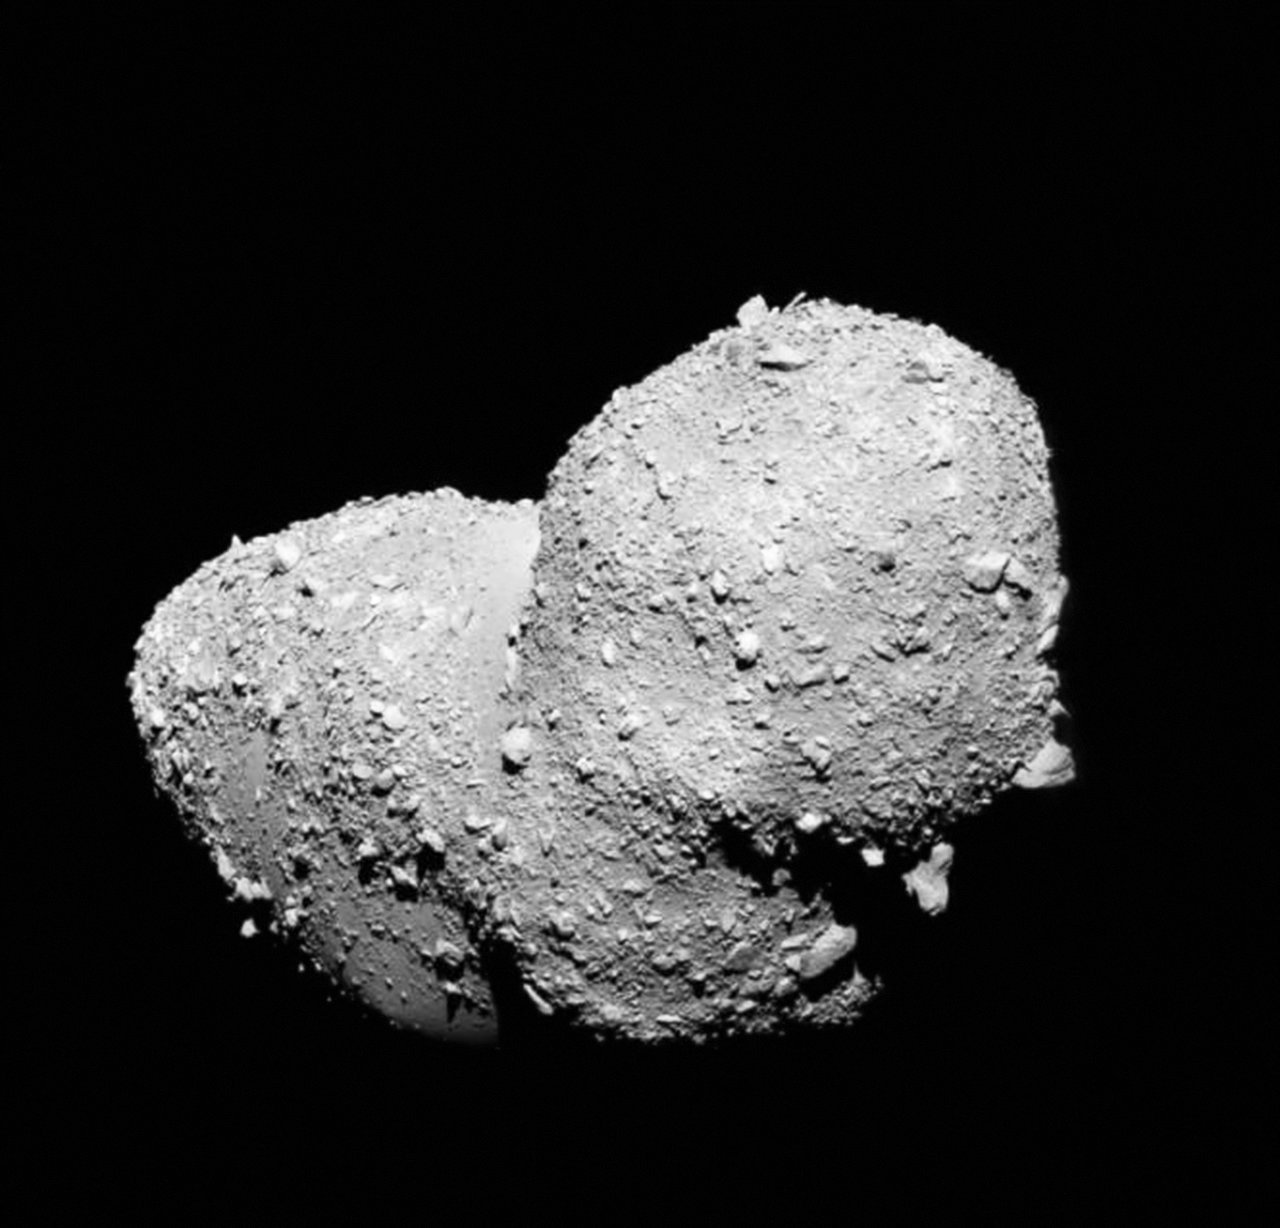
\includegraphics[height=0.3\textheight,width=0.5\textwidth, keepaspectratio]{figures/mathematical_background/eso1405b.jpg}}~
    \subcaptionbox{Comet 67/Churyumov-Gerasimenko\label{fig:67p}}{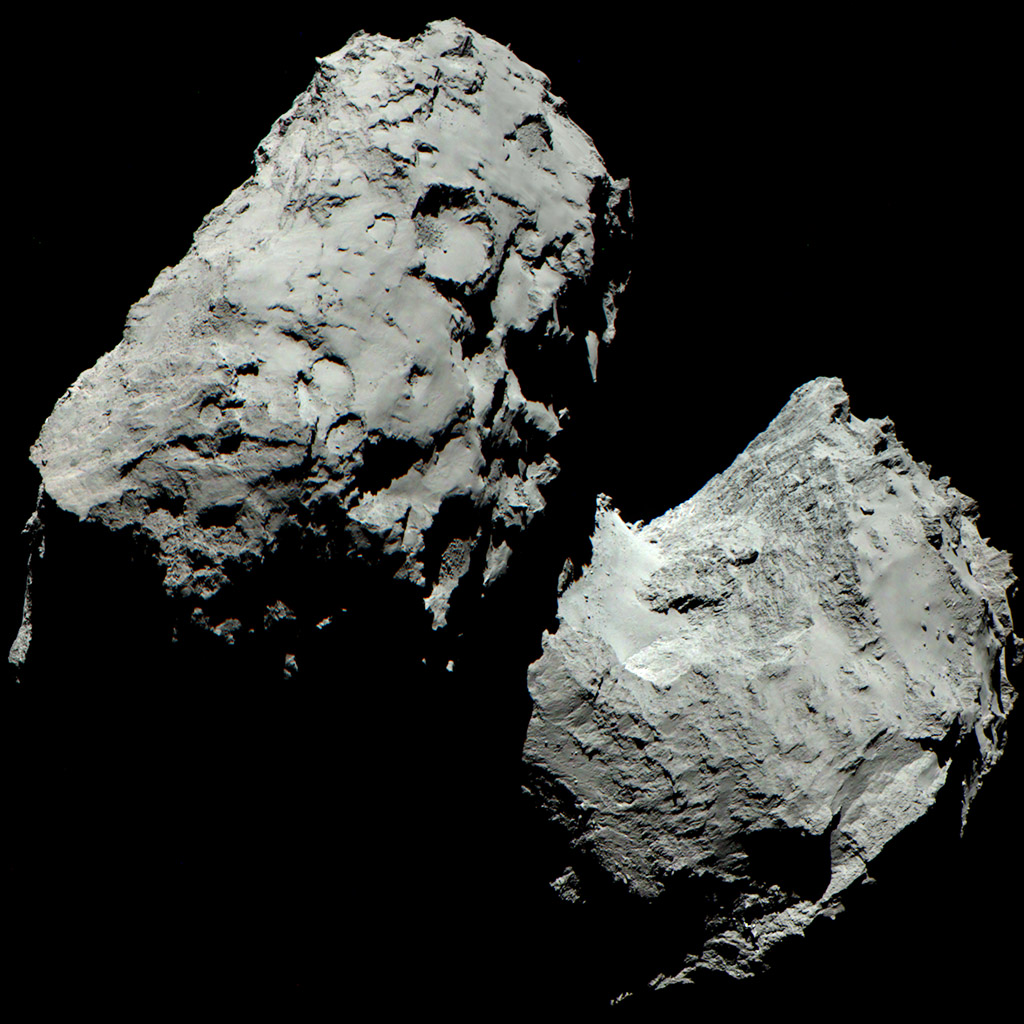
\includegraphics[height=0.3\textheight,width=0.5\textwidth,keepaspectratio]{figures/mathematical_background/comet67pcgin.jpg}}
    \caption{Examples of the non-ellipsoidal shapes of small solar system bodies. Both asteroids and comets will tend to have vastly irregular shapes due to their low mass and violent histories of impacts and collisions~\label{fig:irregular_asteroids}}
\end{figure}
The scientific community describes asteroid shape using the facet-vertex model.
This approach is an efficient representation of the more general notion of a polyhedron from geometry.
In this section, we define the notion of the polyhedron and some specifics of the format used in the astrodynamics community.

A polyhedron is a generalization of a two-dimensional polygon to three-dimensions~\cite{orourke1998}.
It is the region of space with a boundary defined by a surface of a finite number of polygonal faces.
The surface of the polyhedron is composed of three types of primitive objects: zero-dimensional points called vertices, one-dimensional segments called edges, and two-dimensional polygons called faces or facets.
Furthemore, without any loss of generality we assume each face is a convex polygon since any nonconvex face can be divided into smaller convex faces.
A valid polyhedron, in the context of asteroid shape models, must satisfy several constraints.
These constraints define the relationship between each of the types of primitives which make up the polyhedron surface.
The primitives must intersect ``properly'' and the local and global topology must be ``proper''.
For asteroid shape model we further assume that each face is a triangular polygon. 
Again, this does not limit generality as any polygon can be divided into a series of planar triangles.

The intersection of each face must be one of the following:
\begin{itemize}
    \item the faces are disjoint and do not intersect, or
    \item the faces meet at a single vertex, or
    \item the faces share two vertices and a common edge.
\end{itemize}
These intersection constraints automatically ensures that all edgeds and vertices intersect properly.
For example, edges that do not extend across an entire face or faces with penetrate would be improper and invalid.
Some examples of invalid polyhedron are shown in~\cref{fig:improper_polyhedrons}.
\begin{figure}[h]
    \centering
    \subcaptionbox{Point lies on two surfaces\label{fig:two_surfaces}}{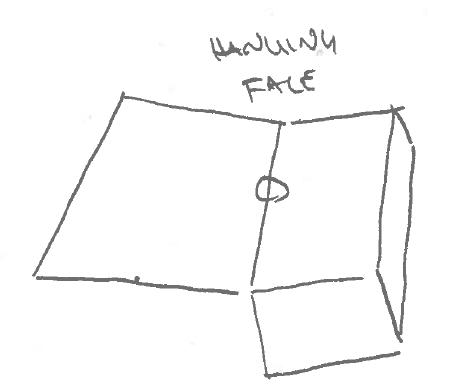
\includegraphics[width=.33\textwidth]{figures/computational_geometry/hanging_face.png}}~
    \subcaptionbox{The neighborhood around this point is not homemorphic to a disk\label{fig:knotted_polyhedron}}{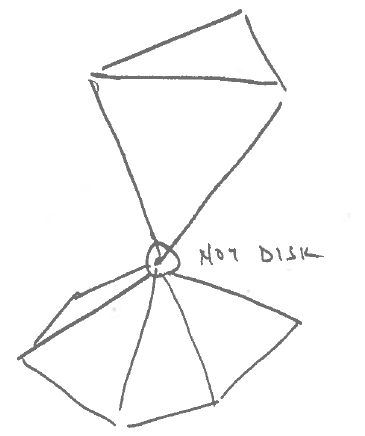
\includegraphics[width=.33\textwidth]{figures/computational_geometry/pinched.png}}~
    \subcaptionbox{The surface is not closed\label{fig:open_polyhedron}}{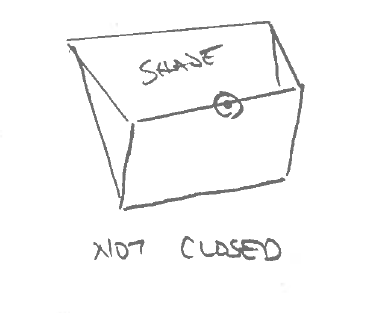
\includegraphics[width=.33\textwidth]{figures/computational_geometry/open.png}}
    \caption{Three example objects which are not polyhedra. For each example, the neighborhood about each point is not homeomorphic to an open disk.~\label{fig:improper_polyhedrons}}
\end{figure}

The second constraint is related to the local topology around each point on the surface of the polyhedron.
In order to be locally proper, the neighborhood about any point on the surface of the polyhedron should be homeomorphic to a two-dimensional disk.
A neighborhood about any point on the surface is defined as an arbitrarily small subset or region of the surface which surrounds the point.
Every point on the surface should have a neighborhood which is topologically equivalent to a two dimensional disk.
The notion of equivalency is mathematically captured using the property of homeomorphism.
A homemorphism between two regions is a continous stretching or bending, without tearing or cutting, from one shape to another.
For example, it is possible to turn a circle into a square by a continuous stretching and bending of the shape.
However, it is not possible to transform a sphere into a torus, as this would require a hole to be created in the surface of the sphere.
The neighborhood about any point on the surface of the polyhedron should be equivalent to that of a two-dimensional disk.
A surface where this true for all points is called a \textit{two-manifold}, of a which the surface of a polyhedron is a subset.

The final constraint is related to the global structure of the surface in contrast to the local neighborhood of a point.
The surface must be connected, closed, and bounded.
In this sense, a connected surface is one where it is possible to travel from one point to any other point of the surface without leaving the surface. 
As a result, this will rule out any shapes with non-connected faces, such as a cube with a hollow interior/surface.
For example, on the outer surface of the cube it is not possible to reach a point on the interior surface. 
Combined with an assumption that there are a finite number of faces automatically ensures a closed and bounded surface. 
Note that these conditions do not in general rule out the possibility of holes passing completely through the object.
For example, a torus, or a donute shape, is also considered a polyhedron.
The key difference between a hole and a cavity is that there are no disconnected surfaces and as a result a polyhedron can have any number of such holes. 
In practice, we tend to limit our analysis to polyhedron with no holes, or with a genus of zero.

% TODO Euler's constant description

\subsection{Polyhedron Data Structures}\label{sec:polyhedron_data_structures}
While the shape of the asteroid will be represented mathematically as a polyhedron, we are still left with the issue of representing this shape in digital form. 
The eventual computational efficiency and memory consumption of the subesequent sections is heavily dependent on the underlying data structure used to represent the surface.
In this section, we review some of the basic requirements and features of any data structure.
In addition, we summarize the ones most popular in the astrodynamics community and the halfedge data structure which we use in this work.

The requirements for any surface/mesh data structure vary between applications and are designed to satisfy both topological and algorithmic requirements.
Some examples of topological considerations are the use of triangular/polygonal facets or the ability to represent manifold/non-manifold meshes.
Examples of algorithmic requirements include a consideration of the types of algorithms/processes that will make use of the data, such as visualization or operations that will modify or additional data to the various faces, edges, and vertices of the mesh.
The choice, and eventual design, of an appropriate data structure is evaluated on its ability to efficiently enable specific operations, such as distance or modification operations.
A wide variety of data structures have been developed to represent general polyhedron surfaces and can be classified as either \textit{face-based} or \textit{edge-based}.

The simplest method to represent a surface mesh is composed to storing the individual vertices which define each face of the surface.
In the specific case of a triangular mesh, this entails storing the three vertex coordinates of each face of the mesh, also called the \textit{face-set}~\cite{botsch2010}.
By assuming that the vertex coordinates are stored as double precision, or \SI{64}{\bit} values, results in \( 3 \cdot 3 \cdot 64 = \SI{576}{\bit} = \SI{72}{\byte}\) per triangular face.
% TODO Add reference to euler's formula
Equivalently, from Euler's formula, there is approximately twice as many faces as vertices, and this \textit{face-set} structure will require on average \SI{144}{\byte} per vertex.
A simple optimization is possible by reducing the redundancy in the representation.
Each vertex will duplicated as many times as the degree of the vertex.
This redundancy can be eliminated by storing a list of vertices, and to define the vertices of each face as an index/reference into this vertex list.
This results in the so called \textit{indexed face set} or \textit{shared-vertex} data structure.
In the case of triangular meshes and using double precision values, each vertex will require \(\SI{192}{\bit} = \SI{24}{\byte}\).
Vertex indices of each face can be stored using single precision, \( \SI{32}{\bit} = \SI{4}{\byte}\), values which resuts in a storage requirement of \( \SI{96}{\bit} = \SI{12}{\byte}\) per triangle.
This type of representation will therefore require on average approximately \( \SI{60}{\byte} \) per vertex, which is half the requirement of the \textit{face-set} data structure.
\begin{figure}
    \centering
    \includegraphics[width=\textwidth]{example-image-golden}
    \caption{Face based data structure look in PMP Fig2.3 or 2.4~\label{fig:face_based_data_structure}}
\end{figure}
Examples of this type of data structure include the \gls{stl}, \gls{obj}, and \gls{off} file formats.

While conceptually simple the face based data structure has several critical drawbacks.
It is difficult to determine the connectivity of individual vertices or faces of the mesh, which makes it ill-suited for most algorithms.
The vast of majority of computational geometry algorithms will require as a minimum~\cite{botsch2010}:
\begin{itemize}
    \item Access to individual vertices, edges and faces, as well as random access to any element.
    \item Enumeration of the edges of a single face.
    \item Access to the adjacent faces of an edge which enables access to the neighboring faces.
    \item Given an edge one must determine the two vertices which define the endpoints.
    \item Given a vertex one must determine all neighboring faces.
\end{itemize}
As a result, any application making use a face based data structure will need to store additional connectivity information in a seperate data structure.

In contrast to face-based structures, edge-based data structures store the connectivity information in the edges or halfedges~\cite{botsch2010,orourke1998,berg2008}.
By splitting each unorientated edge into two orientated halfedges, the halfedge data structure, or also known as the doubly-connected edge list, provides an efficient data structure for mesh based operations.
Each halfedge is ordered in a clockwise fashion around each face, typically such that the face normal is orientated outwards from the mesh.
In addition, each halfedge will also store a reference to:
\begin{itemize}
    \item The vertex it points to, or its target,
    \item its adjacent face,
    \item the next halfedge of the face in a counterclock wise direction,
    \item the previous halfedge of the face
    \item the opposite or incident halfedge.
\end{itemize}
In addition, each face stores the reference to one of its halfedges, while each vertex stores an outgoing halfedge. 
The halfedge data structure will require more memory in contrast to face based approaches it offers several advantages which make it ideal for computational geometry operations.

\subsubsection{Halfedge Data Structure}\label{sec:halfedge_data_structure}
A halfedge data structure allows us to iterate through all elements, vertices, edge, halfedge, or face, in a simple manner.
In addition, the halfge edge data structure can store arbitrary polygon meshes.
Furthermore, additional data can be attached to the elements as each is store explicitly.
Finally, the halfedge data structure allows for simple manipulation and modification of the underlying mesh, enabling operations such as mesh subdivision or simplification.
There are a number of publicly avaiable implementations of the halfedge data structure~\cite{cgalproject2018,botsch2002}.
We utilize the \texttt{Surface\_mesh} data structure implemented within the Computational Geometry Algorithms Library~\cite{sieger2011}.
This provides a well defined and highly optimzed data structure for the representation of the polyhedron shape of the asteroid.
Furthermore, the ability to incorporate additional properties enables us to efficently compute the polyheron potential model.
\begin{figure}
    \centering
    \includegraphics[width=\textwidth]{example-image-golden}
    \caption{Halfedge data structure look in PMP Fig3.4~\label{fig:halfedge_data_structure}}
\end{figure}

\begin{figure}
    \centering
    \includegraphics[width=\textwidth]{example-image-golden}
    \caption{Iterating over 1 ring of a vertex}
\end{figure}
% TODO Describe the halfedge data structure and Surface_mesh in more detail

\subsubsection{Wavefront OBJ files}
The OBJ format is a geometry definition file format used for a variety of computer modeling applications, and is regularly used by the asteroid community~\cite{neese2004}.
The basic format of the file is an ASCII file where the first \( N_v\) lines begin with \texttt{v} and define the three components of a vertex in the body fixed reference frame.
The following \( N_f\) lines begin with \texttt{f} and define the three indices of the vertices that make up the face.
The numbering of the vertices is implicitly defined by the order listed in the file, i.e. the vertices are defined from \( 1 \) to \( N_v\).
There are two main assumptions used by the asteroid community.
First, each face is triangular and second, the vertices are numbered in a counterclockwise fashion about each face.
This allows the outward facing normal to each face to be uniquely defined without any additional data.

This polyhedron model, captured using the OBJ format, allows for a much larger class of potential object shapes. 
The accuracy of the shape model can be arbitrarily improved by incorporating additional vertices and faces, which increase the resolution of the model in regions of high complexity.
The polyhedron model can capture arbitrary depressions, ridges, or holes through the asteroid.
Small bodies typically lack sufficient mass to create regular, spherical shapes, and exhibit a large variety in resulting shapes such as the examples shown in~\cref{fig:asteroid_shape}.
\begin{figure}
    \centering
    \subcaptionbox{4769 Castalia\label{fig:castalia}}{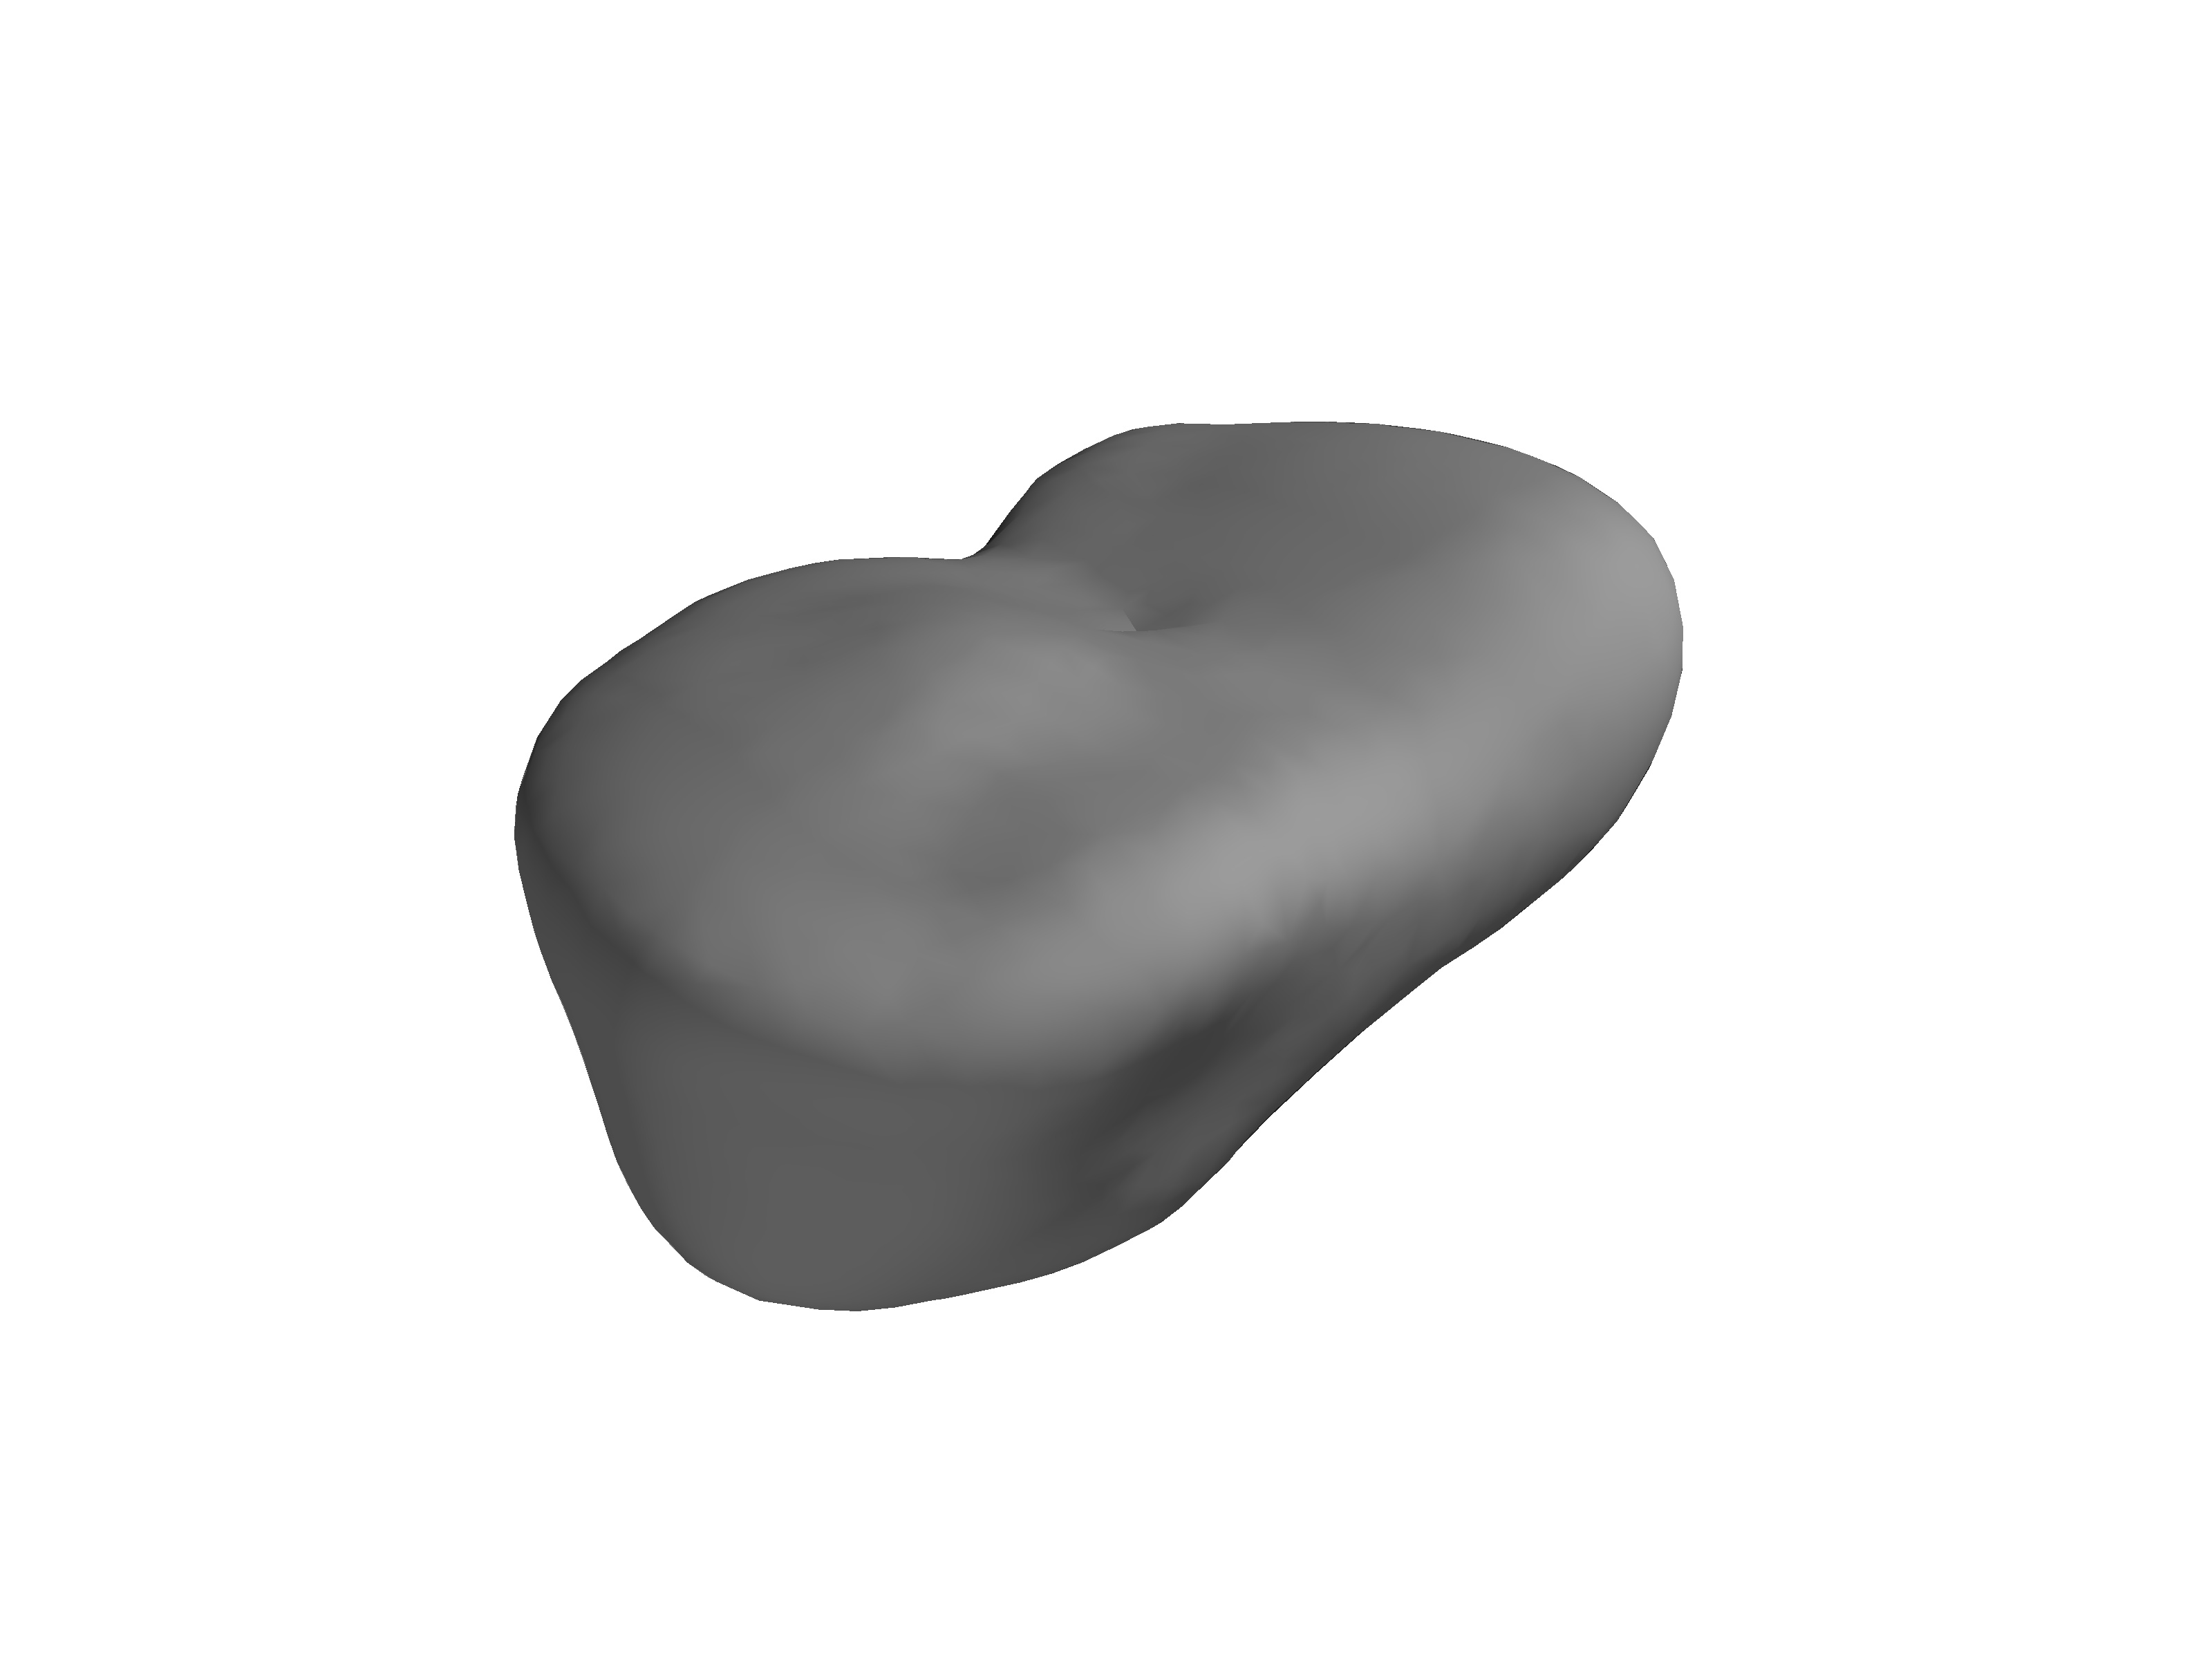
\includegraphics[width=0.33\textwidth]{figures/mathematical_background/castalia_isometric.jpg}}~
    \subcaptionbox{Geographus\label{fig:geographus}}{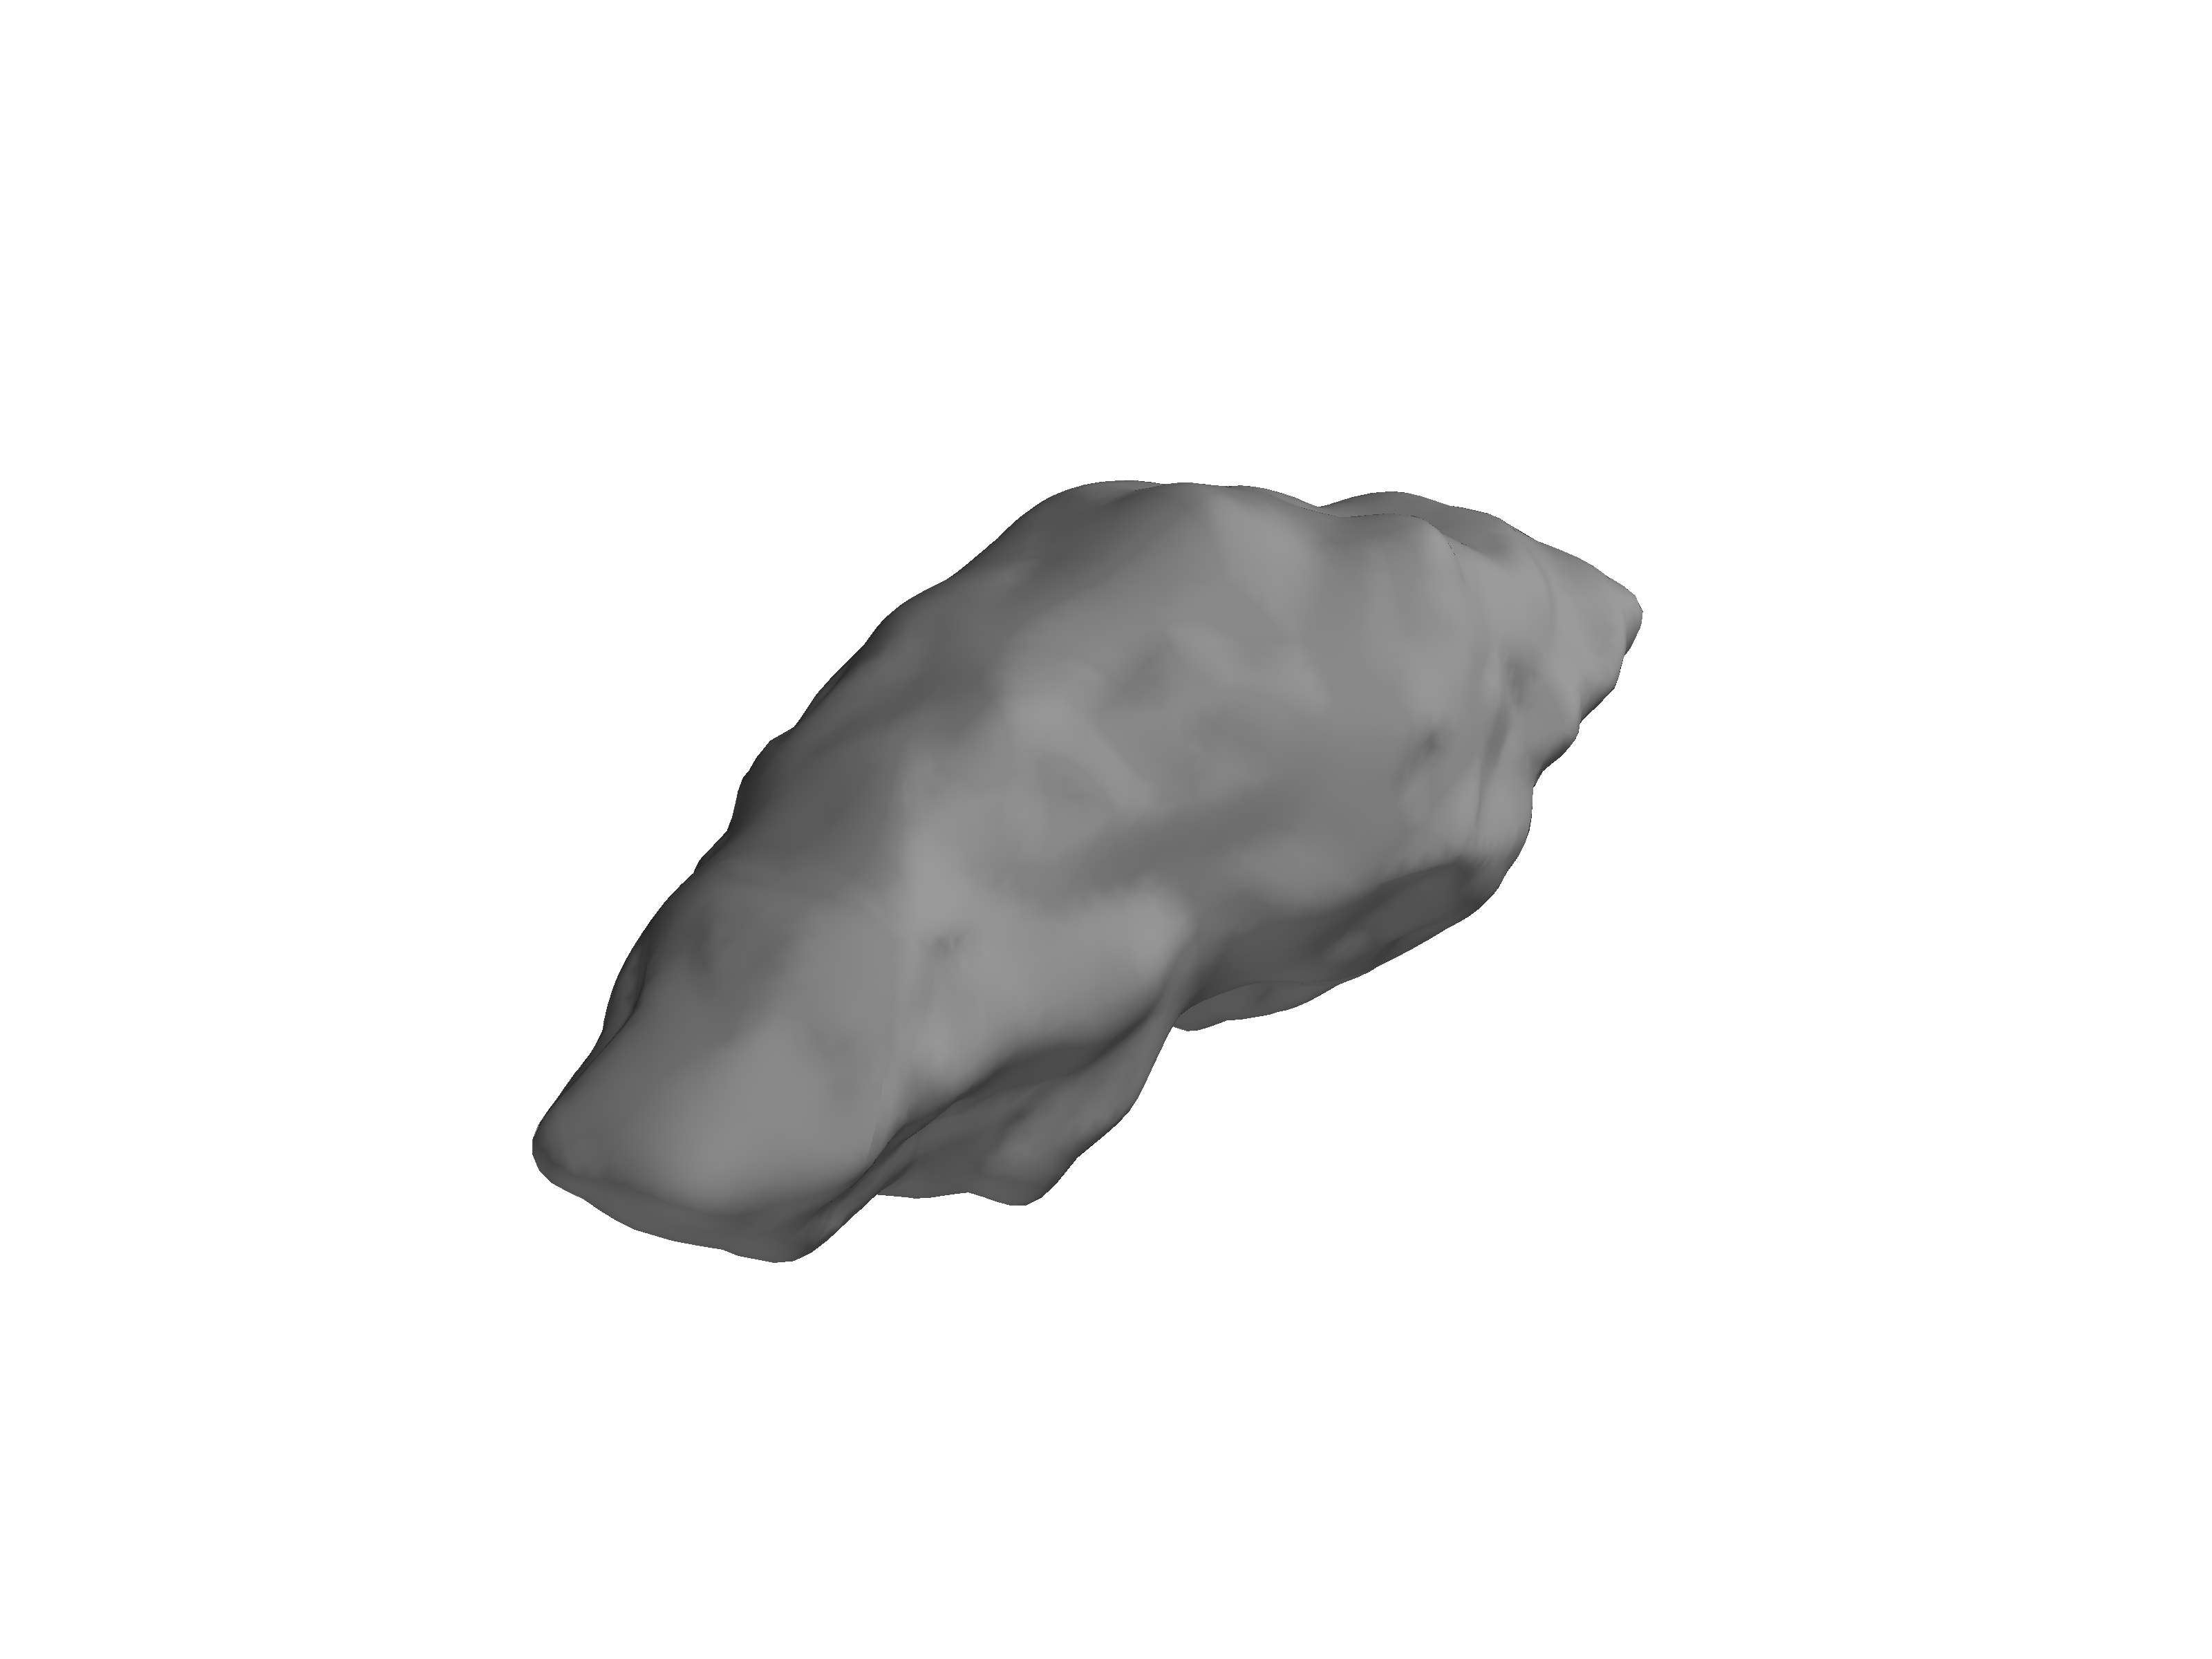
\includegraphics[width=0.33\textwidth]{figures/mathematical_background/geographus_isometric.jpg}}~
    \subcaptionbox{Golevka\label{fig:golevka}}{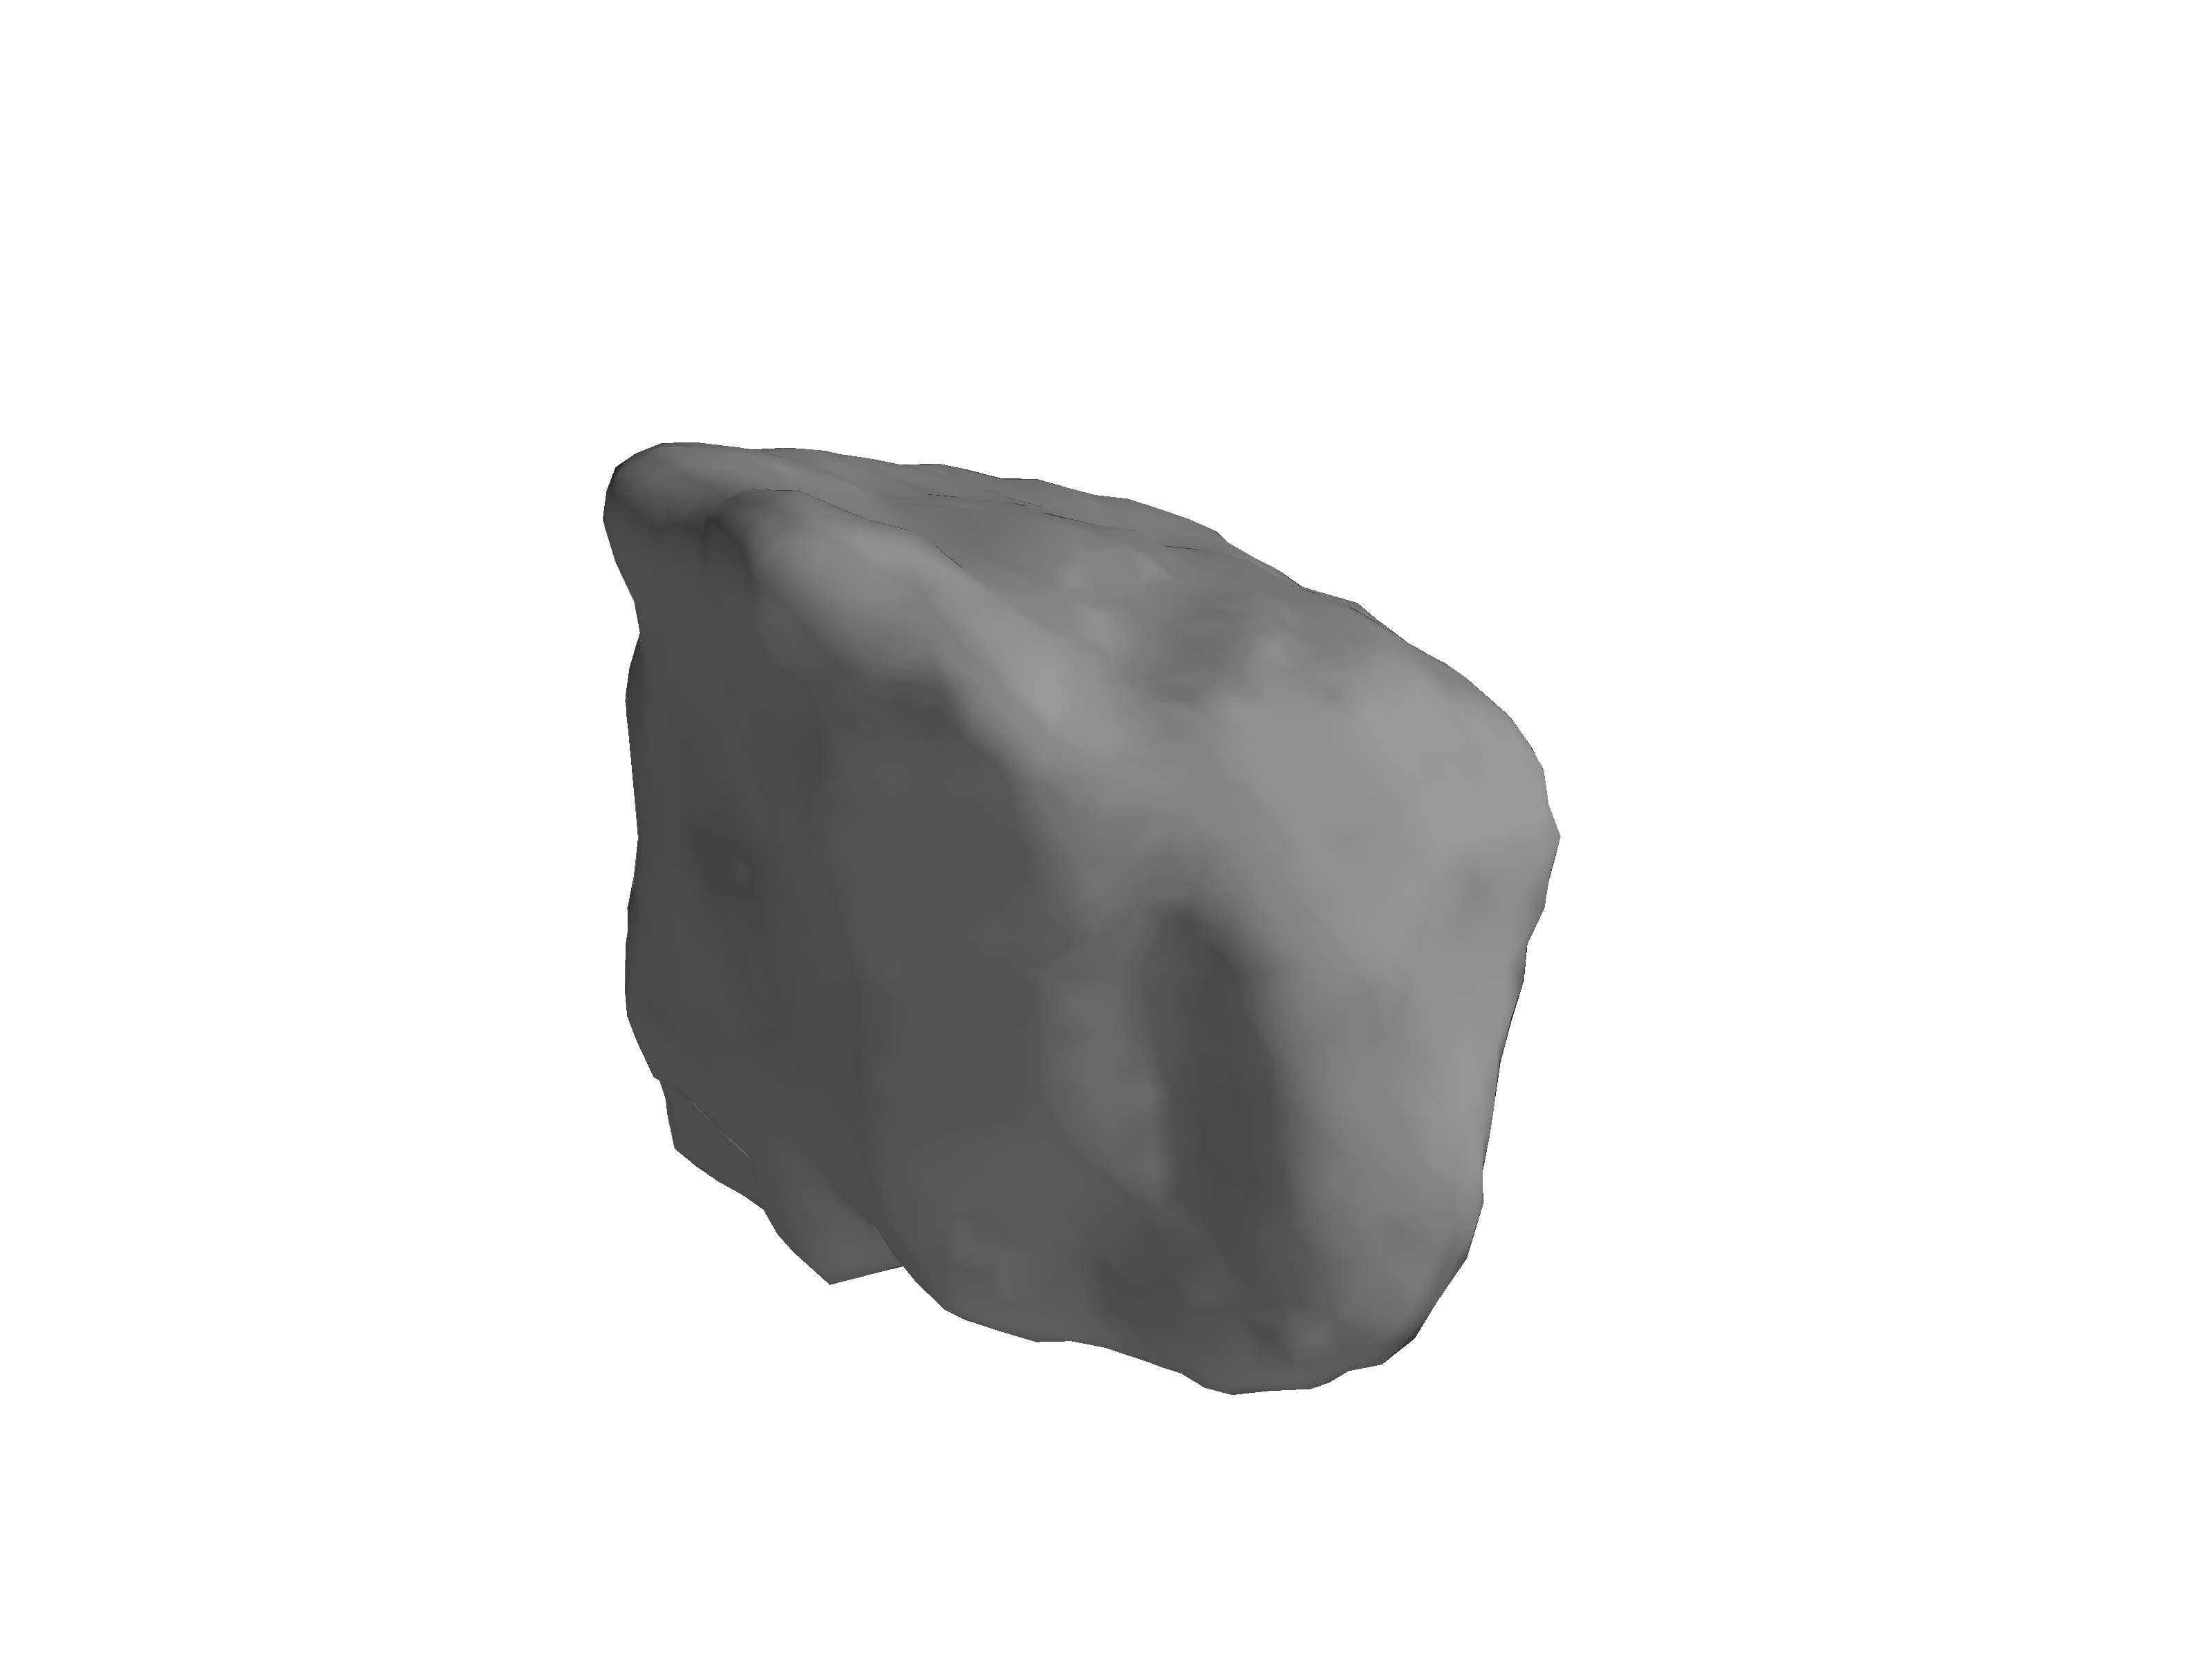
\includegraphics[width=0.33\textwidth]{figures/mathematical_background/golevka_isometric.jpg}}
    \caption{Polyhedron Shape Models for several asteroids~\label{fig:asteroid_shape}}
\end{figure}
Polyhedron shape models are available for several asteroids~\cite{neese2004,gaskell2008b}.
The quality and resolution is dependent on the measurement available of the body.
\Cref{fig:itokawa_radar} shows a polyhedron model of asteroid 25143 Itokawa based on ground radar measurements~\cite{neese2004}.
This model is composed of \num{6098} vertices and \num{12192} faces and captures the general ellipsoidal shape of the asteroid.
However, ground based measurements are unable to provide the resolution required to capture the fine details or even the asymmetry of asteroid Itokawa.
In contrast,~\cref{fig:itokawa_insitu} shows the model derived from in-situ measurements from optical sensor of the Hyabusa spacecraft~\cite{gaskell2008a}.
It is composed of \num{1579014} vertices and \num{3145728} faces and is able to capture small surface features such as boulders.
\begin{figure}
    \centering
    \subcaptionbox{25143 Itokawa Radar Model\label{fig:itokawa_radar}}{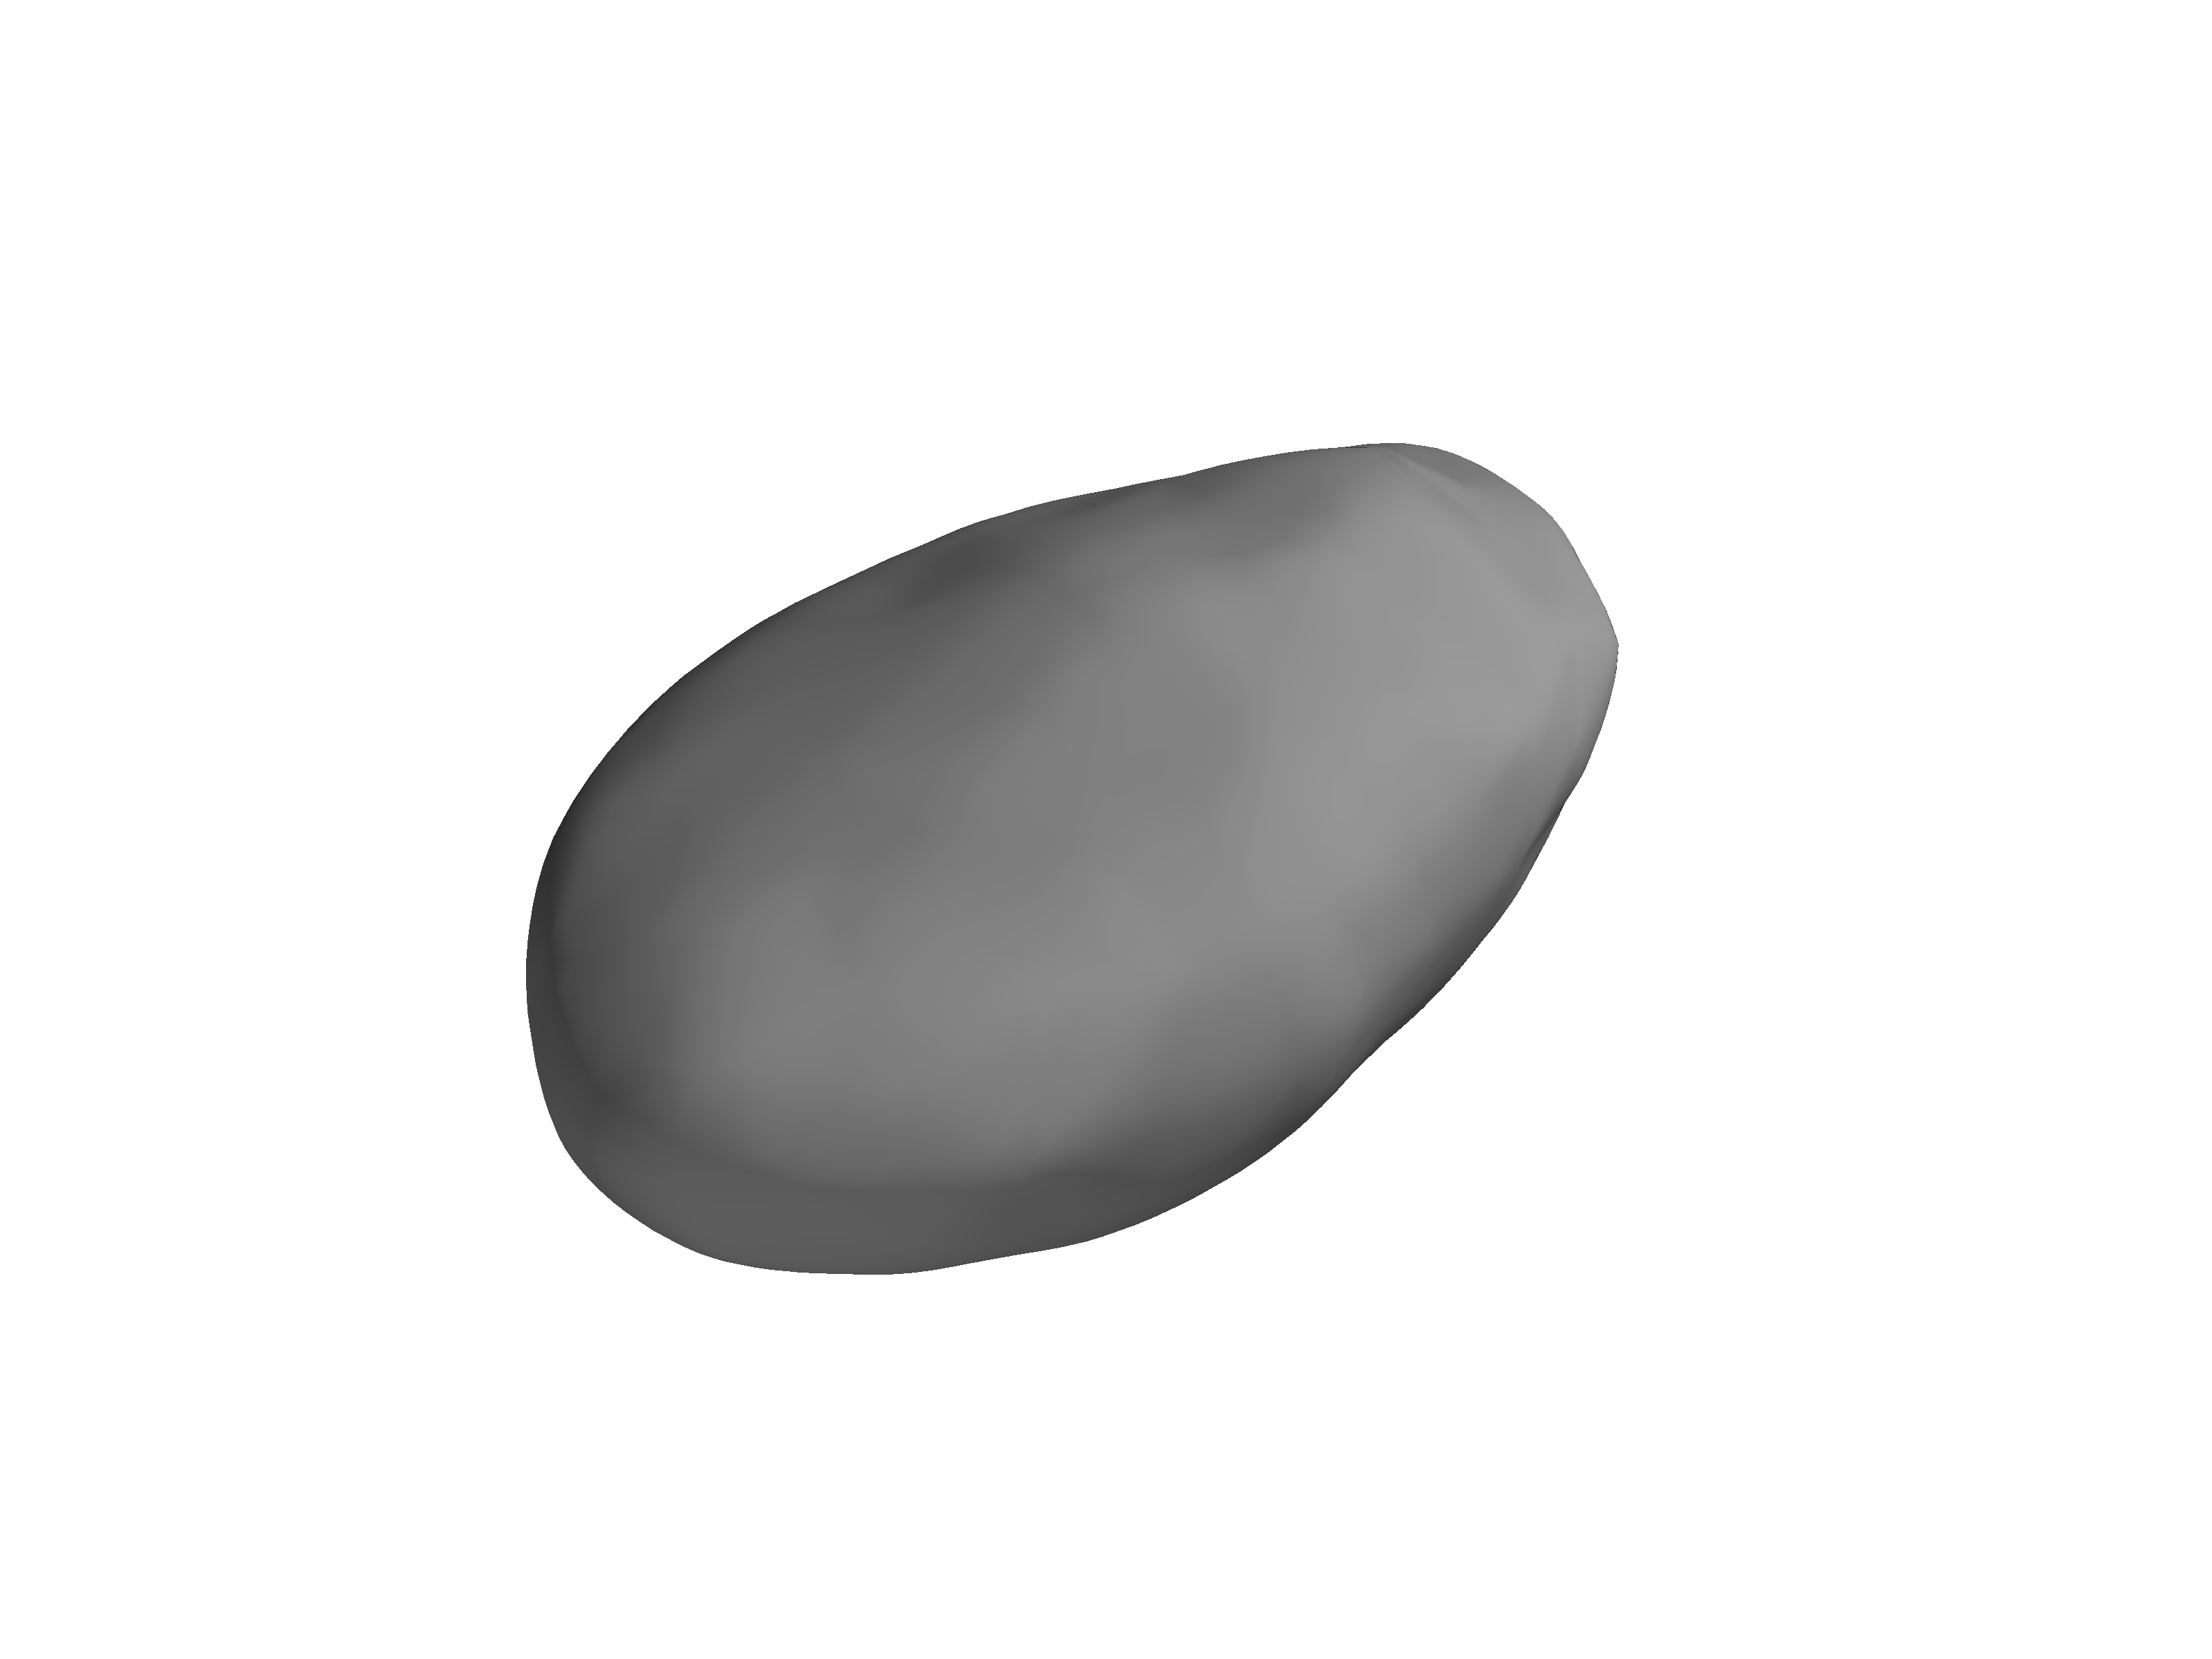
\includegraphics[width=0.5\textwidth]{figures/mathematical_background/itokawa_radar_isometric.jpg}}~
    \subcaptionbox{25143 Itokawa In-Situ Model\label{fig:itokawa_insitu}}{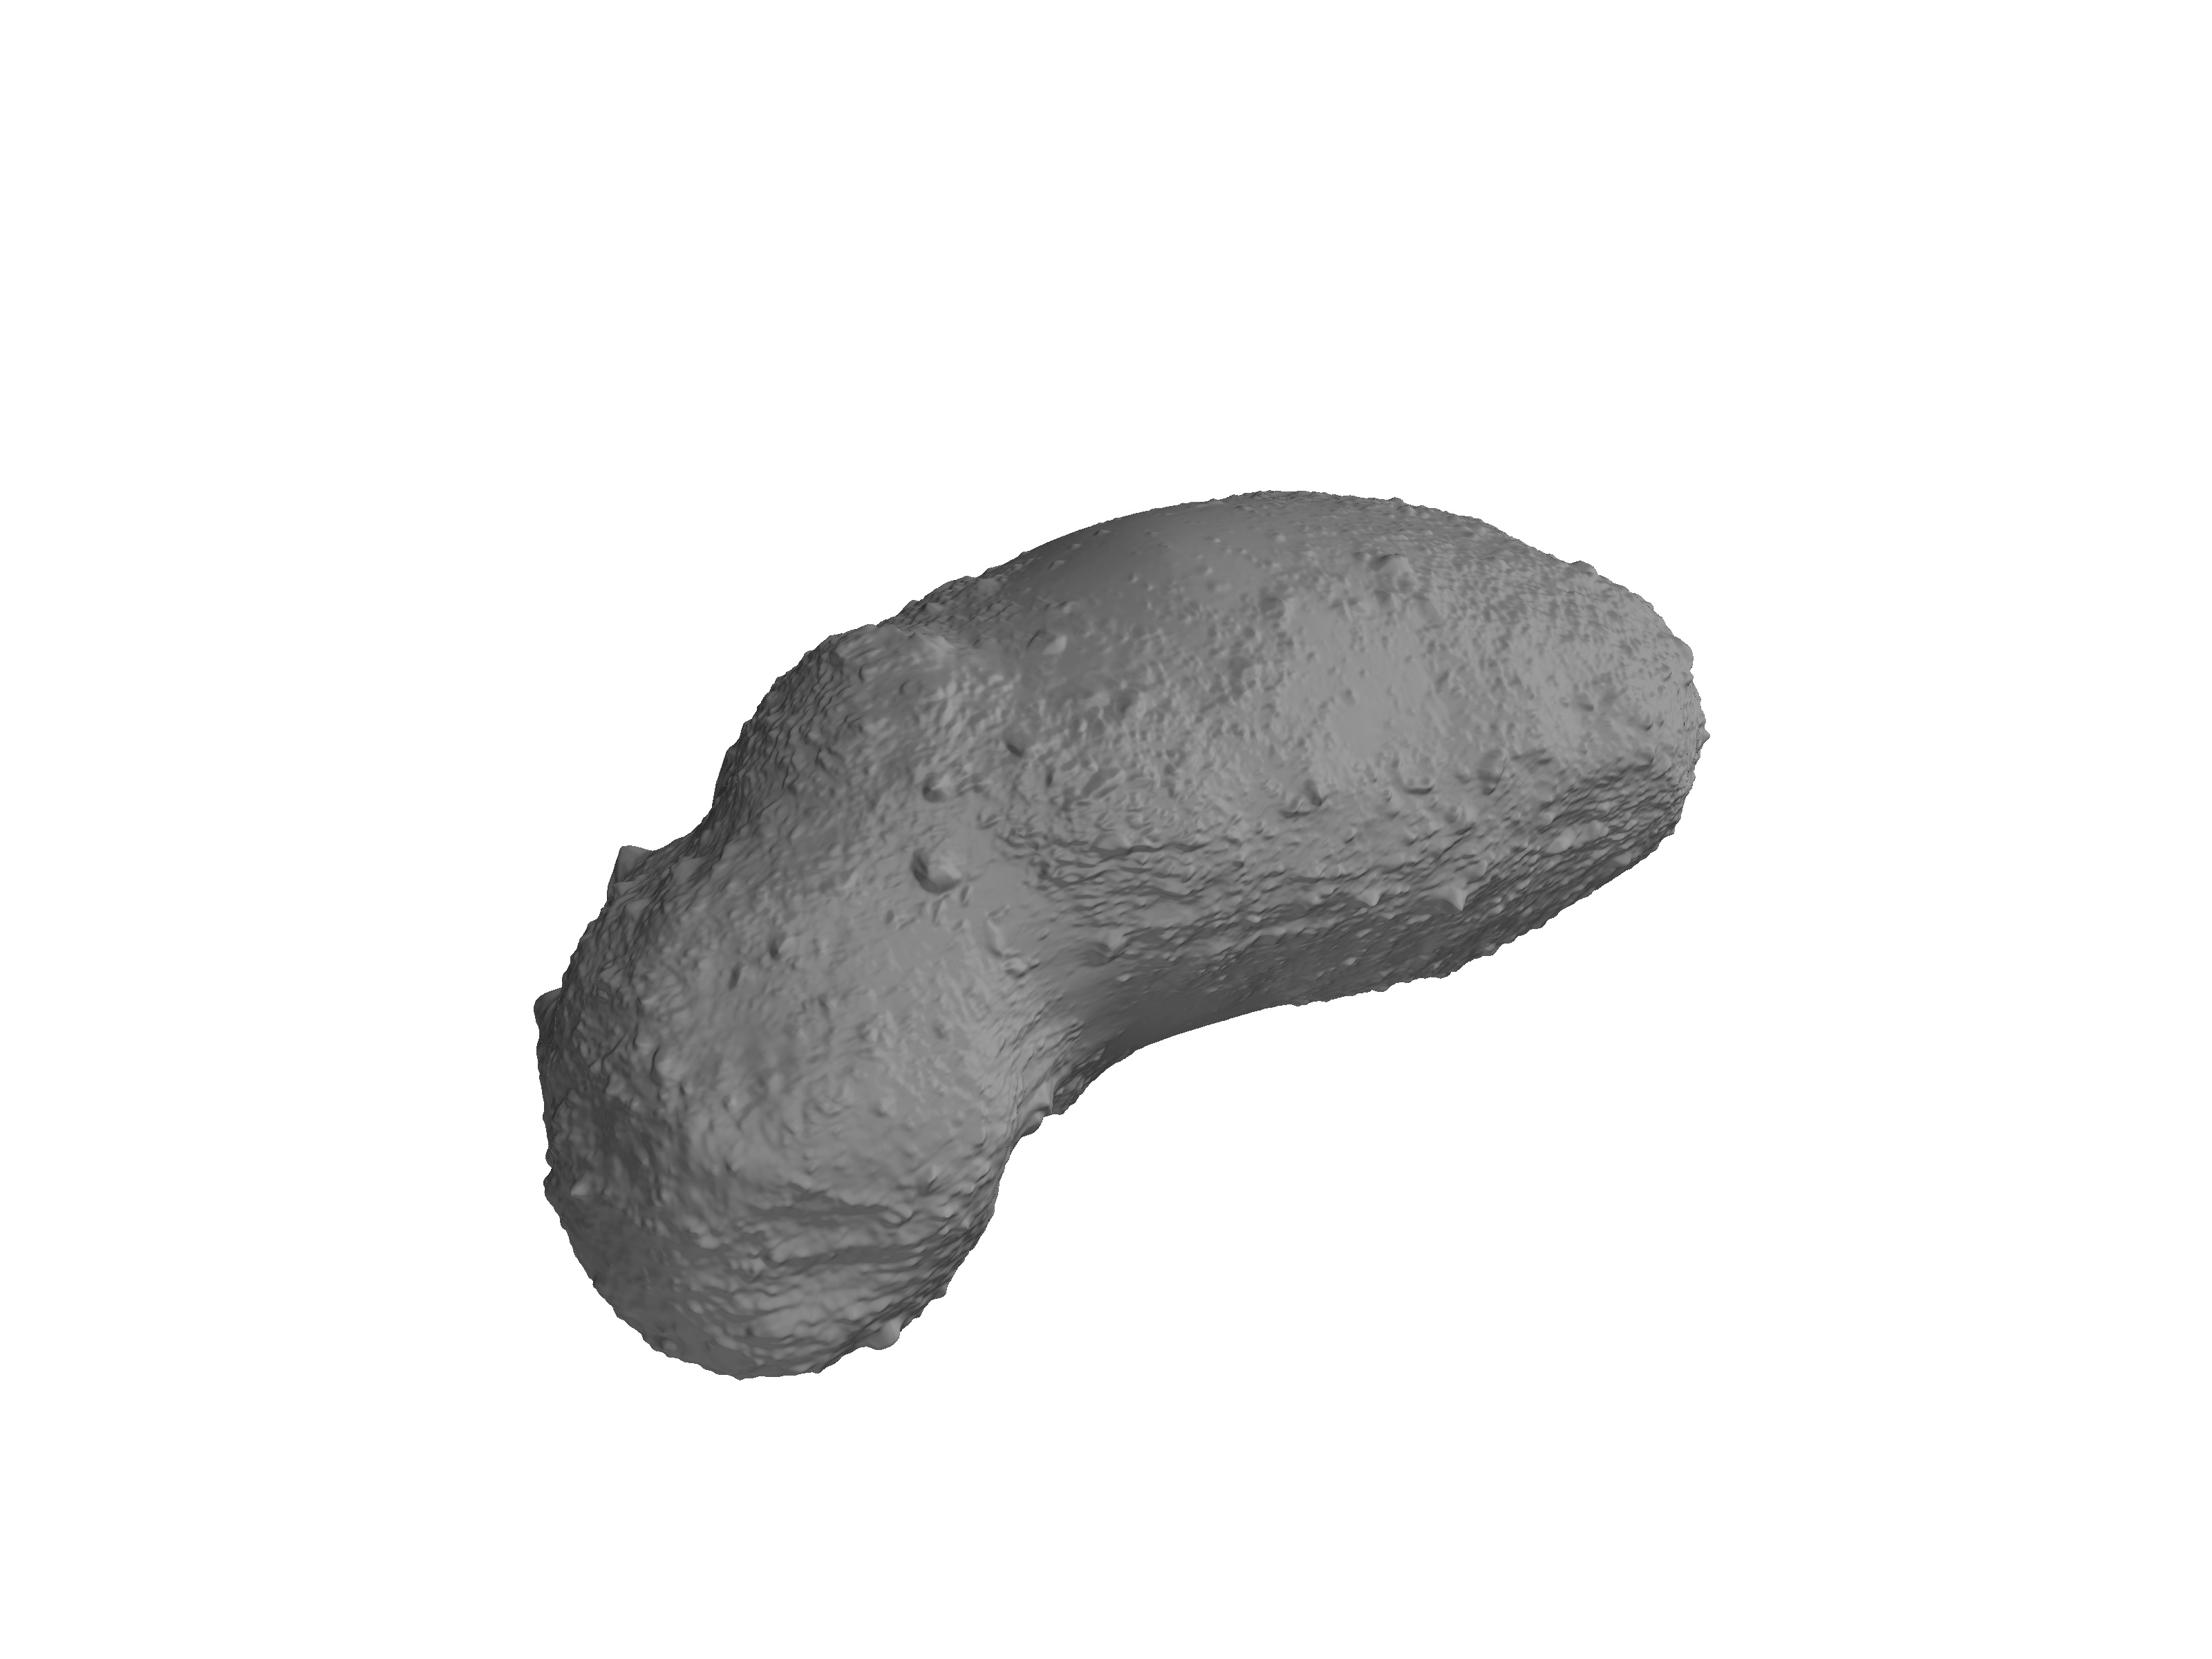
\includegraphics[width=0.5\textwidth]{figures/mathematical_background/itokawa_isometric.jpg}}
    \caption[Comparison of Radar and In-situ Itokawa models]{Comparision of polyhedron models of 25143 Itokawa based on ground based radar or in-situ measurements.
        The ground based model can capture the rough ellipsoidal shape but does not capture fine surface details.}
\end{figure}
From this simple example, it is clear that prior to the arrival of a spacecraft the shape and surface knowledge of an asteroid is limited.
\subsection{Polyhedra}

A polyhedron is a generalization of a two-dimensional polygon to three-dimensions.
It is the region of space with a boundary defined by a surface of a finite number of polygonal faces.
The surface of the polyhedron is composed of three types of primitive objects: zero-dimensional points called vertices, one-dimensional segments called edges, and two-dimensional polygons called faces or facets.
Furthemore, without any loss of generality we assume each face is a convex polygon since any nonconvex face can be divided into smaller convex faces.
A valid polyhedron in the context of asteroid shape models must satisfy several constraints.
These constraints define the relationship between each of the types of primitives which make up the polyhedron surface.
The primitives must intersect ``properly'', the local and global topology must be ``proper''.
For asteroid shape model we further assume that each face is a triangular polygon. 
Again, this does not limit generality as any polygon can be divided into a series of planar triangles.

The intersection of each face must be one of the following:
\begin{itemize}
    \item the faces are disjoint and do not intersect, or
    \item the faces meet at a single vertex, or
    \item the faces share two vertices and a common edge.
\end{itemize}
This constraint automatically ensures that all edgeds and vertices intersect properly.
Improper intersection would penetrating faces and faces that intersect improperly. 
Such as an edge not extending across an entire face.

The second constraint is related to the local topology around each point of the polyhedron.
In order to be locally proper, the neighborhood about any point on the surface of the polyhedron should be homeomorphic to a two-dimensional disk.
A neighborhood about any point on the surface is defined as an arbitrarily small subset or region of the surface which surrounds the point.
Every point on the surface should have a neighborhood which is topologically equivalent to a two dimensional disk.
The notion of equivalency is mathematically captured using the property of \gls{homeomorphism}.
A homemorphism between two regions is a continous stretching or bending, without tearing or cutting, from one shape to another.
For example, it is possible to turn a circle into a square by a continuous stretching and bending of the shape.
However, it is not possible to transform a sphere into a torus, as this would require a hole to be created in the surface of the sphere.
This constraint will exlude objects that are not proper polyhedrons, for example those shown in~\cref{fig:improper_polyhedrons}.

In a neighborhood about any point on the surface of the polyhedron should be equivalent to that of a two-dimensional disk.
A surface where this true for all points is called a \textit{two-manifold}, of a which the surface of a polyhedron is a subset.

The final constraint is related to the global structure of the surface in contrast to the local neighborhood of a point.
The surface must be connected, closed, and bounded.
In this sense, a connected surface is one where it is possible to travel from one point to any other point of the surface without leaving the surface. 
As a result, this will rule out any shapes with non-connected faces, such as a cube with a hollow interior/surface.
For example, on the outer surface of the cube it is not possible to reach a point on the interior surface. 
Combined with an assumption that there are a finite number of faces automatically ensures a closed and bounded surface. 
Note that these conditions do not in general rule out the possibility of holes passing completely through the object.
For example, a torus, or a donute shape, is also considered a polyhedron.
The key difference between a hole and a cavity is that there are no disconnected surfaces and as a result a polyhedron can have any number of such holes. 
In practice, we tend to limit our analysis to polyhedron with no holes, or with a genus of zero.

\begin{itemize}
    \item Talk about 1-manifold and homeomorphism to a disk
    \item Define neighborhood of each point (open adn closed balls)
\end{itemize}

Global topology
\begin{itemize}
    \item Connected closed and bounded
    \item talk about closed holes (torus) and the genus of a polyhedron
    \item Give precise definitions about connected and topological spaces.
    \item Look in ~\cite{morris1988,hatcher2002}
\end{itemize}

Platonic solids
\begin{itemize}
    \item Talk about platonic solids and Euler's equation
\end{itemize}

\section{Measurement Model}

In the computer graphics field a major problem is the determination of which objects are visible to the user.
In a method similar to the photographic process in reverse, for each pixel of the image a ray is cast towards the scene and the intersections of this ray with any objects is recorded.
The first object which intersects the ray is defined as visible while those beyond would be occluded.
Given this intersection point, the surface normal is computed and surface shading can be determined to render the scene.

Our problem is of a similar nature to that of the computer graphics domain.
Given the model of an asteroid, its shape model, we wish to first simulate measurements of the surface. 
In order to simulate these methods, we must also implement a ray casting algorithm that will find the intersection of a measurement from the spacecraft to the surface. 

We assume that the spacecraft is located at \gls{rho} in the asteroid fixed frame.
The camera/sensor is aligned with \gls{view_axis} in the spacecraft fixed frame.
An additional vector, defined as the up axis \gls{up_axis}, finally the standard basis is completed with \( \gls{view_axis} \times \gls{up_axis} \) which defines a reference frame attached to the image plane of the sensor.
Furthermore, we model the the laser ranging sensor as having a fixed field of view defined by the angles \( \gls{fov_h}, \gls{fov_v}\), defining the vertical and horizontal fields of view.
In order to simulate depth measurements we need to compute the vectors associated with image sensor in the asteroid frame. 
Given the view axis, and a chosen distance \gls{view_distance}, we can define a viewing \gls{frustum} associated with the sensor. 
We can compute the vectors associated with the maximum extents of the far plane as follows.
The half height and width of the far plane, at a distance \( d \), is computed as
\begin{align}
    H = d \tan \frac{\alpha}{2} , \\
    W = d \tan \frac{\beta}{2} .
\end{align}
From these values, the extents of the far plane are defined by the vectors
\begin{align}
    A = \hat d + H \hat u - W \hat r , \\
    B = \hat d + H \hat u + W \hat r, \\
    C = \hat d - H \hat  u + W \hat r, \\
    D = \hat d - H \hat u - W \hat r.
\end{align}

% TODO: Explain more about ray casting
\begin{itemize}
    \item Give some background on raycasting and where it is used
    \item Discuss the method used in VTK (Binary space partitioning or Oriented bounding boxes)
\end{itemize}

\subsection{Laser Range Finder on Spacecraft}

% TODO: Talk about laser range finders on spacecraft
Absolute distance measuring devices are a crucial sensor in spacecraft rendezvous or landing applications.
In addition, they are a critical component for spacecraft operating near asteroids.
Activate ranging devices allow for precise measurments of the surface shape and enable accurate and safe surface landing~\cite{berry2013}.

The basic principle central to all active range-finding devices is to transmit a signal onto an object and process the returned signal to determine the distance~\cite{amann2001}.
The transmitted signal can fall into one of three categories: radio, ultrasonic, or optical.
The benefit of optical signal is that they can be highly focused to enable high resolution distance measurments
Optical distance measurment, such as laser range finders, can be further divided into three categories based on the method of operation: interferometry, \gls{tof}, or triangulation.
In this section, we'll briefly summarize the principles of operation of optical distance measurement devices, and highlight their specific uses with respect to spacecraft missions to asteroids.

\subsection{Time of Flight Distance Measurement}
Originally developed for military and surveying application, the basic principle of laser ranging is based on utilizing the fixed speed of light to measure distance.
The time required for a pulse of energy to travel from the transmitter to the object and return is measured, \( t_d \). 
Meausuring this round trip \gls{tof} and using the speed of light, approximately \( c = \SI{30}{\centi\meter\per\nano\second}\), allows one to easily compute the range to the object as
\begin{align}
    \rho = \frac{t_d}{2 c}. 
\end{align}
A main benefit of the \gls{tof} ranging system is that a single pulse of energy is sufficient to accurately determine distance to meter level precision in the case of spacecraft or millimeter level in industrial applications~\cite{zuber1997,cole1998,amann2001}.

A pulsed \gls{tof} laser distance device consists of a laser transmitter which emits pulses with a duration between \SIrange{5}{50}{\nano\second}~\cite{amann2001}.
The emitted light pulse triggers a start signal in the onboard timing device and the reflected energy from the object provides the stop command.
A block diagram of the laser range finder is show in~\cref{fig:lidar_block_diagram}.
\begin{figure}[htbp]
    %TODO Update figure with a tikz block diagram
    \centering
    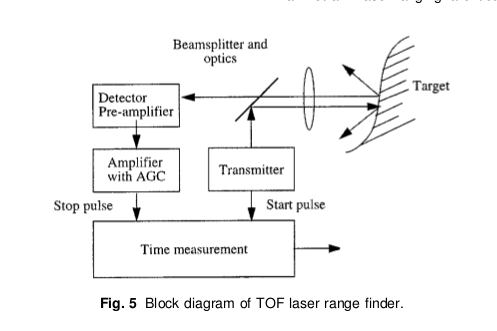
\includegraphics[width=\textwidth]{figures/raycasting/block_diagram.png}
    \caption{\textbf{CHANGE TO TIKZ} Block diagram of \gls{tof} laser range finder\label{fig:lidar_block_diagram}}
\end{figure}
A wide variety of lasers are used depending on the intended measurments range.
In the spacecraft case, laser providing peak energy in the range of \SI{15}{\mega\joule} are often required to measure distance of over \SI{50}{\kilo\meter}~\cite{berry2013}.

The laser range finder is frequently equipped with angle encoders to enable the definition of the position of the measurement point with respect to the sensor. 
Mechanical scanning is performed using a control system which  either move the entire laser range finder or only the measuring beam.
Focal plane scanning is another approach which reduces the mechanical complexity of a mechanical scanning system.
The laser energy illuminates the entire field of view on the surface.
An array of detectors are aranged to view the surface.
Each detector only views a portion of the total field of view and the signals are analyzed in the time domain.
Using this methodology, the system can simulataneously measure distance in multiple directions without any moving parts~\cite{amann2001}.

\subsection{Asteroid Mapping Operations}

Precise relative navigation and landing near asteroids is critically dependent on an accurate knowledge of the shape of the body.
The fine topological structure of the surface is not possible without a spacecraft in the vicinity of the asteroid.
From ground  based measurments, such as radar or optical telescopes, it is only possible to achieve a coarse model of asteroid, such as a triaxial ellipsoid representation~\cite{hudson1994}.
The size and shape of asteroid presents critical information into the thermal and collisional histories and more critically into their internal structure~\cite{cole1998}.

Typical missions spend months after arrival at an asteorid mapping and measuring the surface.
During this mapping phase, which requires upwards of \num{6} months, the spacecraft must maintain a specific trajectory and attitude to ensure best measurements of the surface~\cite{cheng2002,barnouin-jha2008}.
Both the spacecraft orbit and it's attitude is constrained to best satsify the competing requirements of the range measurements, spacecraft power, and Earth based communications.
These measurements are then sent back to Earth, and combined with the spacecraft orbit determination to simulateously estimate the asteroid shape, mass, gravity field, spin state, and spacecraft state.

Look at miller2002 for more detail and discuss that here

% TODO Discuss how the shape of an asteroid is determined in pracice currently
\begin{itemize}
    \item Talk about ground based imaging and citations (radar/optical)
    \item tlak about best knowledge of asteroid before arrival is a ellipsoid model (first mometn)
    \item Talk about sending missions to asteroids with laser altimeters
    \item Months of mapping and ground based OD
\end{itemize}

\section{Incremental Radius modification}\label{sec:radius_update}



One of the first main tasks for any spacecraft mission to an asteroid is to generate an estimate of the asteroid shape.
This shape model is used for a variety of purposes, such as the polyhedron potential model, like that presented in~\cref{sec:polyhedron_potential} or landing site section and guidance.
We assume that upon arrival at a target body, the spacecraft contains an initial estimate for the shape of the asteroid.
This shape can be a coarse estimate computed from ground measurements or it can be a triaxial ellipsoid based on the semimajor axes of the asteroid, such as that shown in~\cref{fig:start} which represents the maximum axes for asteroid Castalia.
Additionally, we assume that the shape estimate is closed and a triangular faceted surface mesh, emulating those used in practice to represent asteroids.
Furthermore, the number of vertices in the estimate can be scaled according to the resulting acccuracy or computational capabilities.
For example,~\cref{fig:uniform_mesh} demonstrates two surface mesh representation for a triaxial ellipsoid at varying levels of detail. 
A wide variety of algorithms are available to generate a near uniformly spaced mesh for an arbitrary surface~\cite{persson2004,boissonnat2005}.
\begin{figure}[htbp]
    \centering
    \subcaptionbox{Coarse Uniform Mesh\label{fig:coarse_uniform_mesh}}{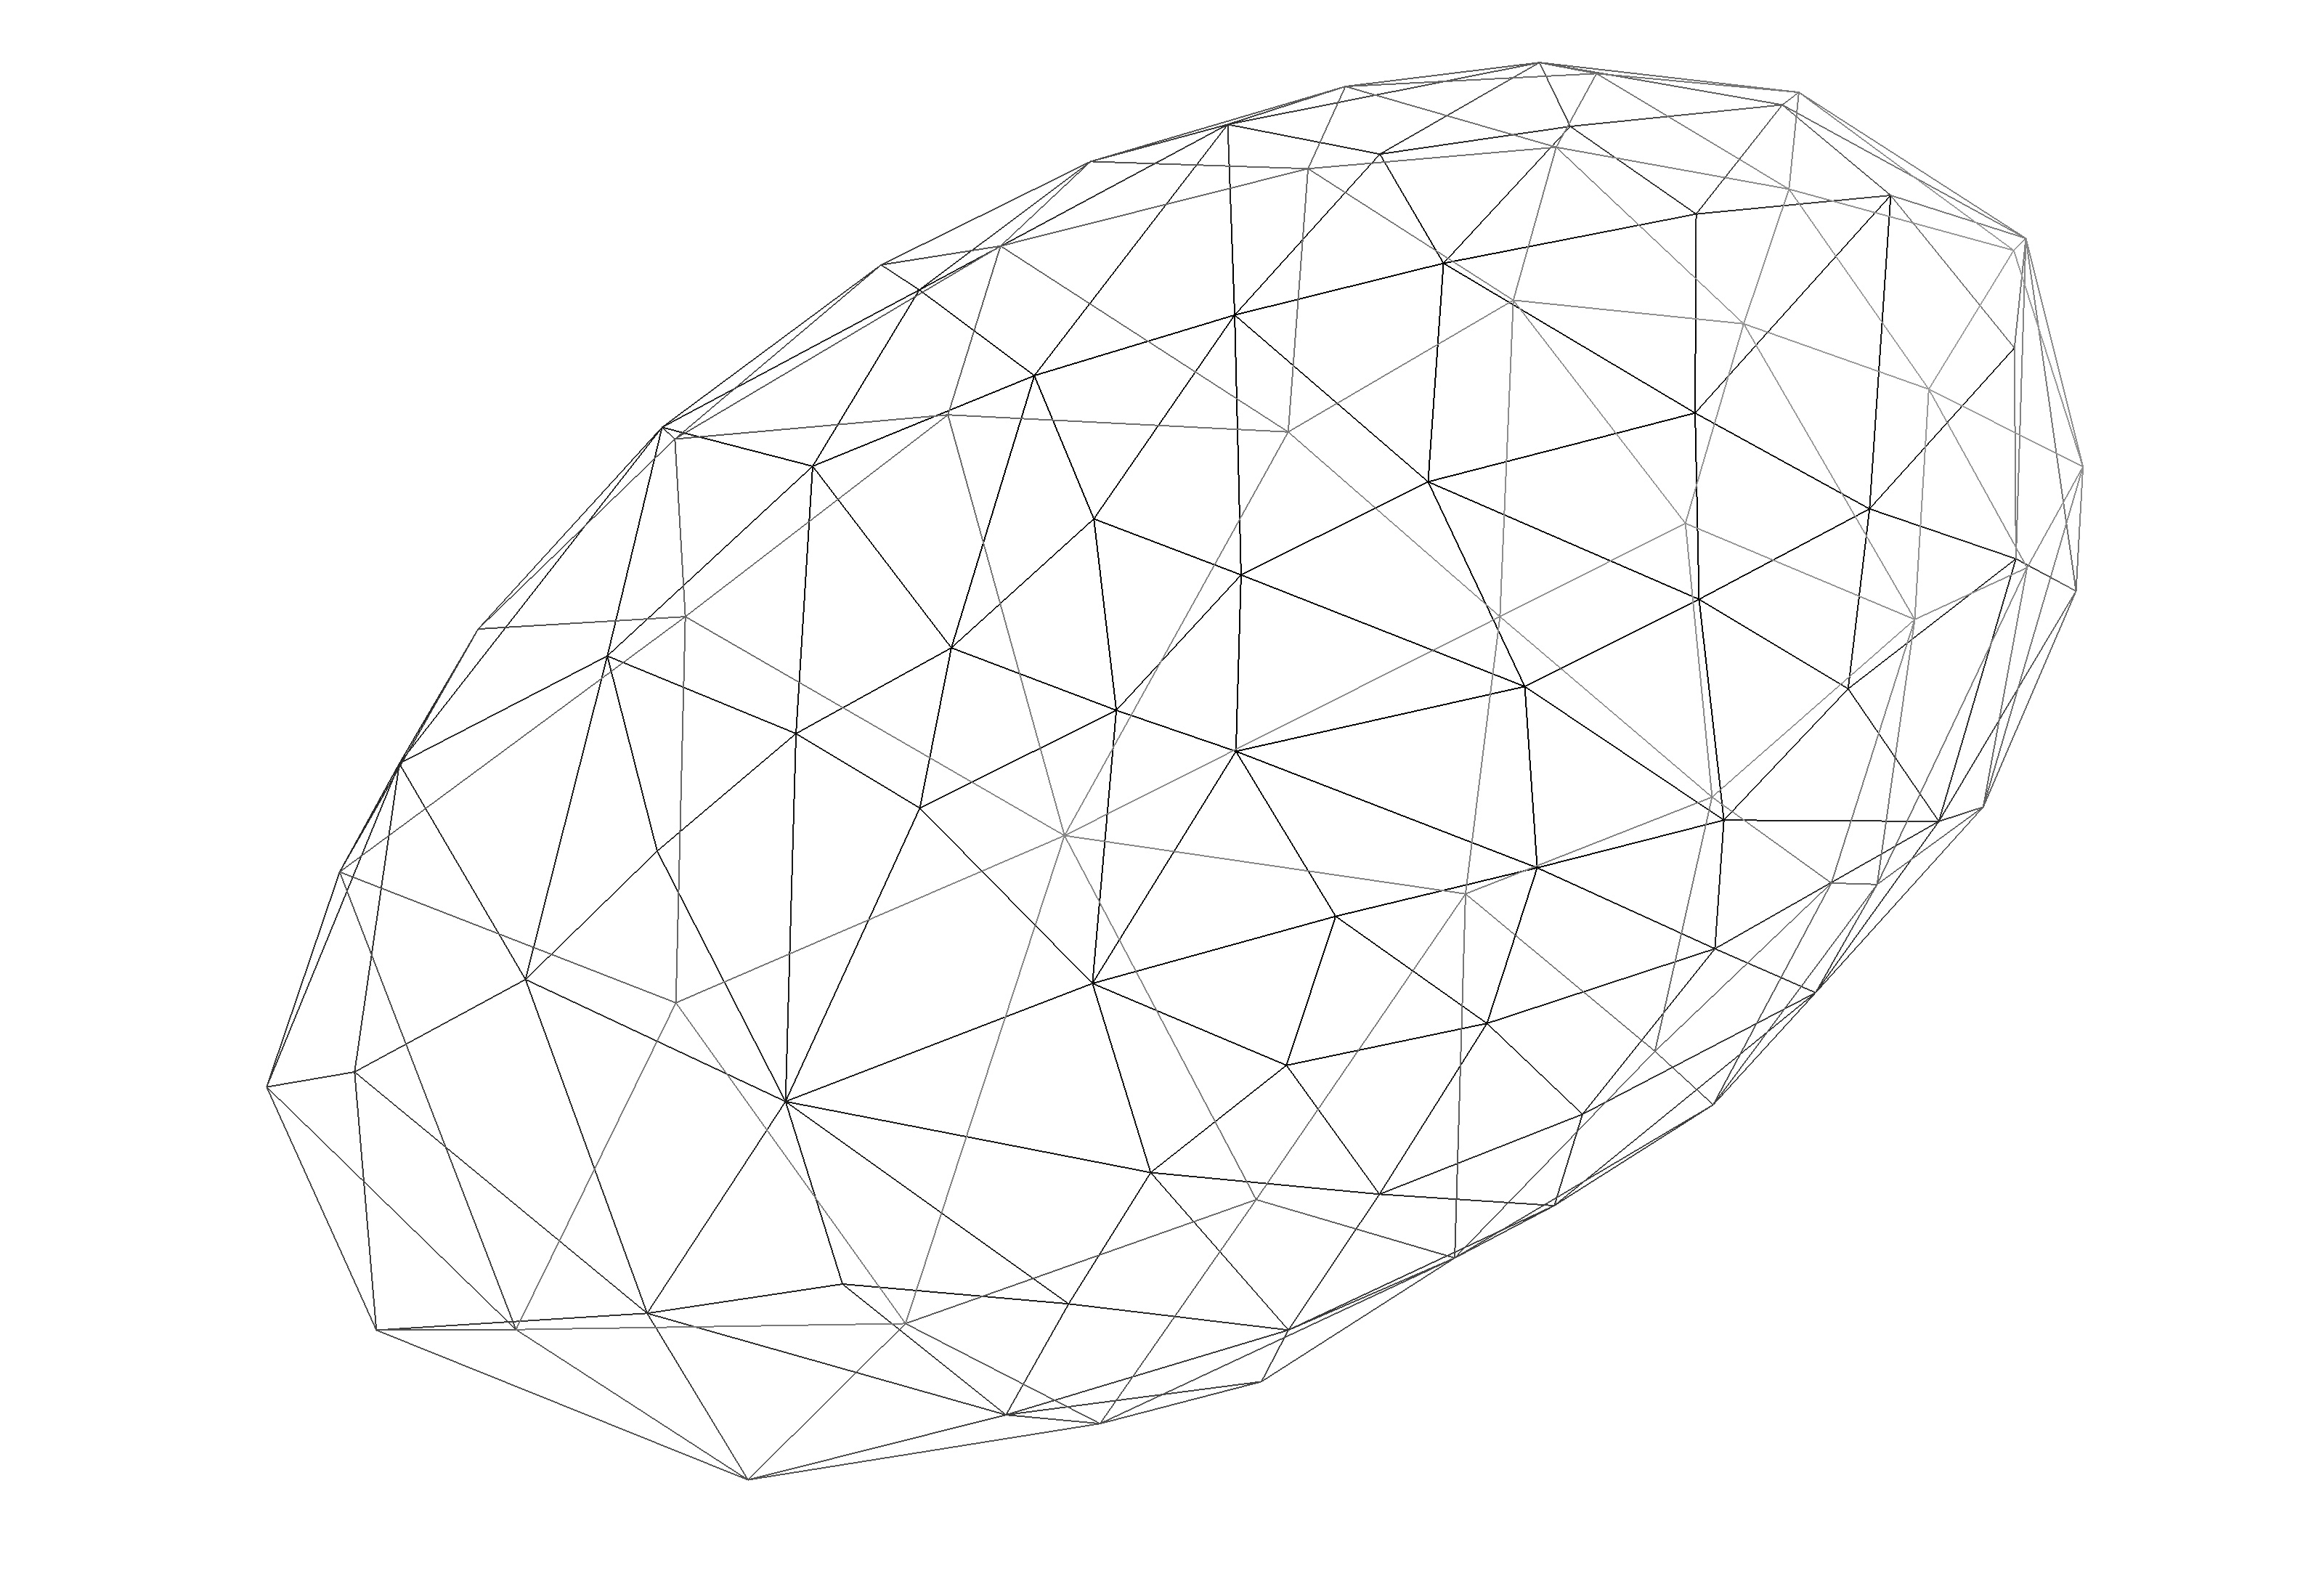
\includegraphics[width=0.5\textwidth]{figures/computational_geometry/uniform_mesh_coarse.jpg}}~
    \subcaptionbox{Fine Uniform Meesh\label{fig:fine_uniform_mesh}}{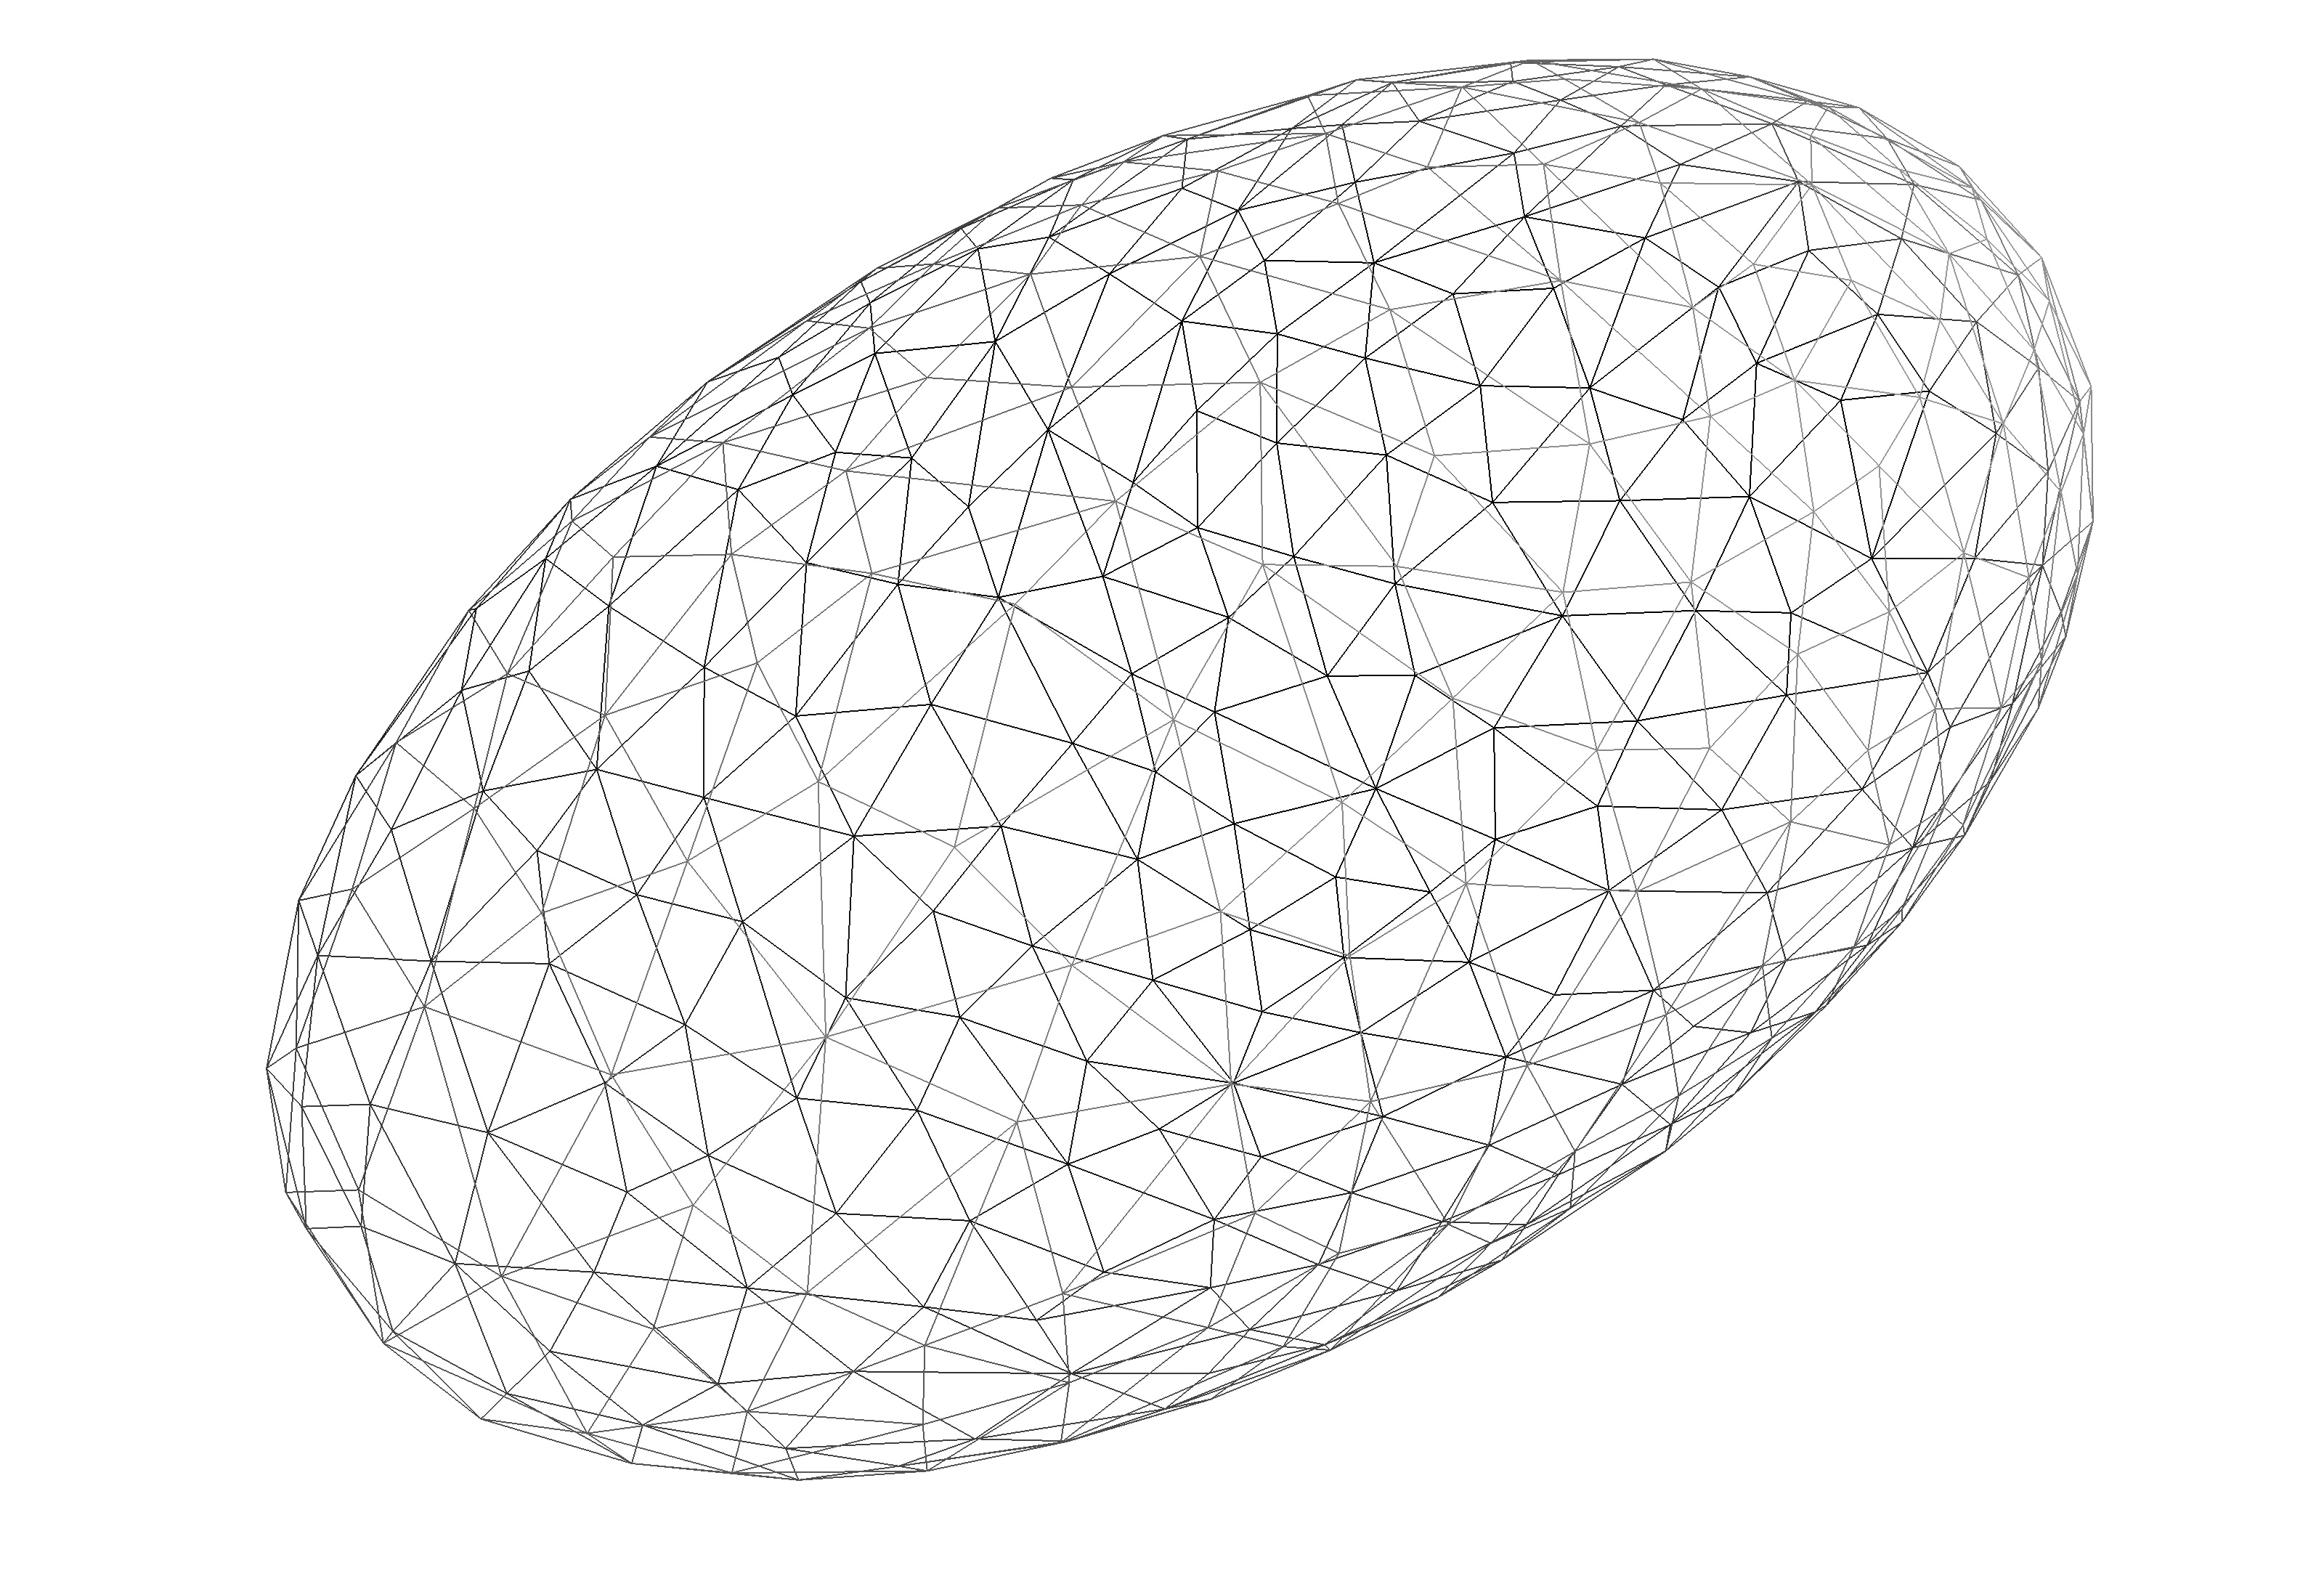
\includegraphics[width=0.5\textwidth]{figures/computational_geometry/uniform_mesh_fine.jpg}}
    \caption{Examples of Resolution of Uniform Meshes of Triaxial Ellipsoid~\label{fig:uniform_mesh}}
\end{figure}

\begin{figure}
    \centering
    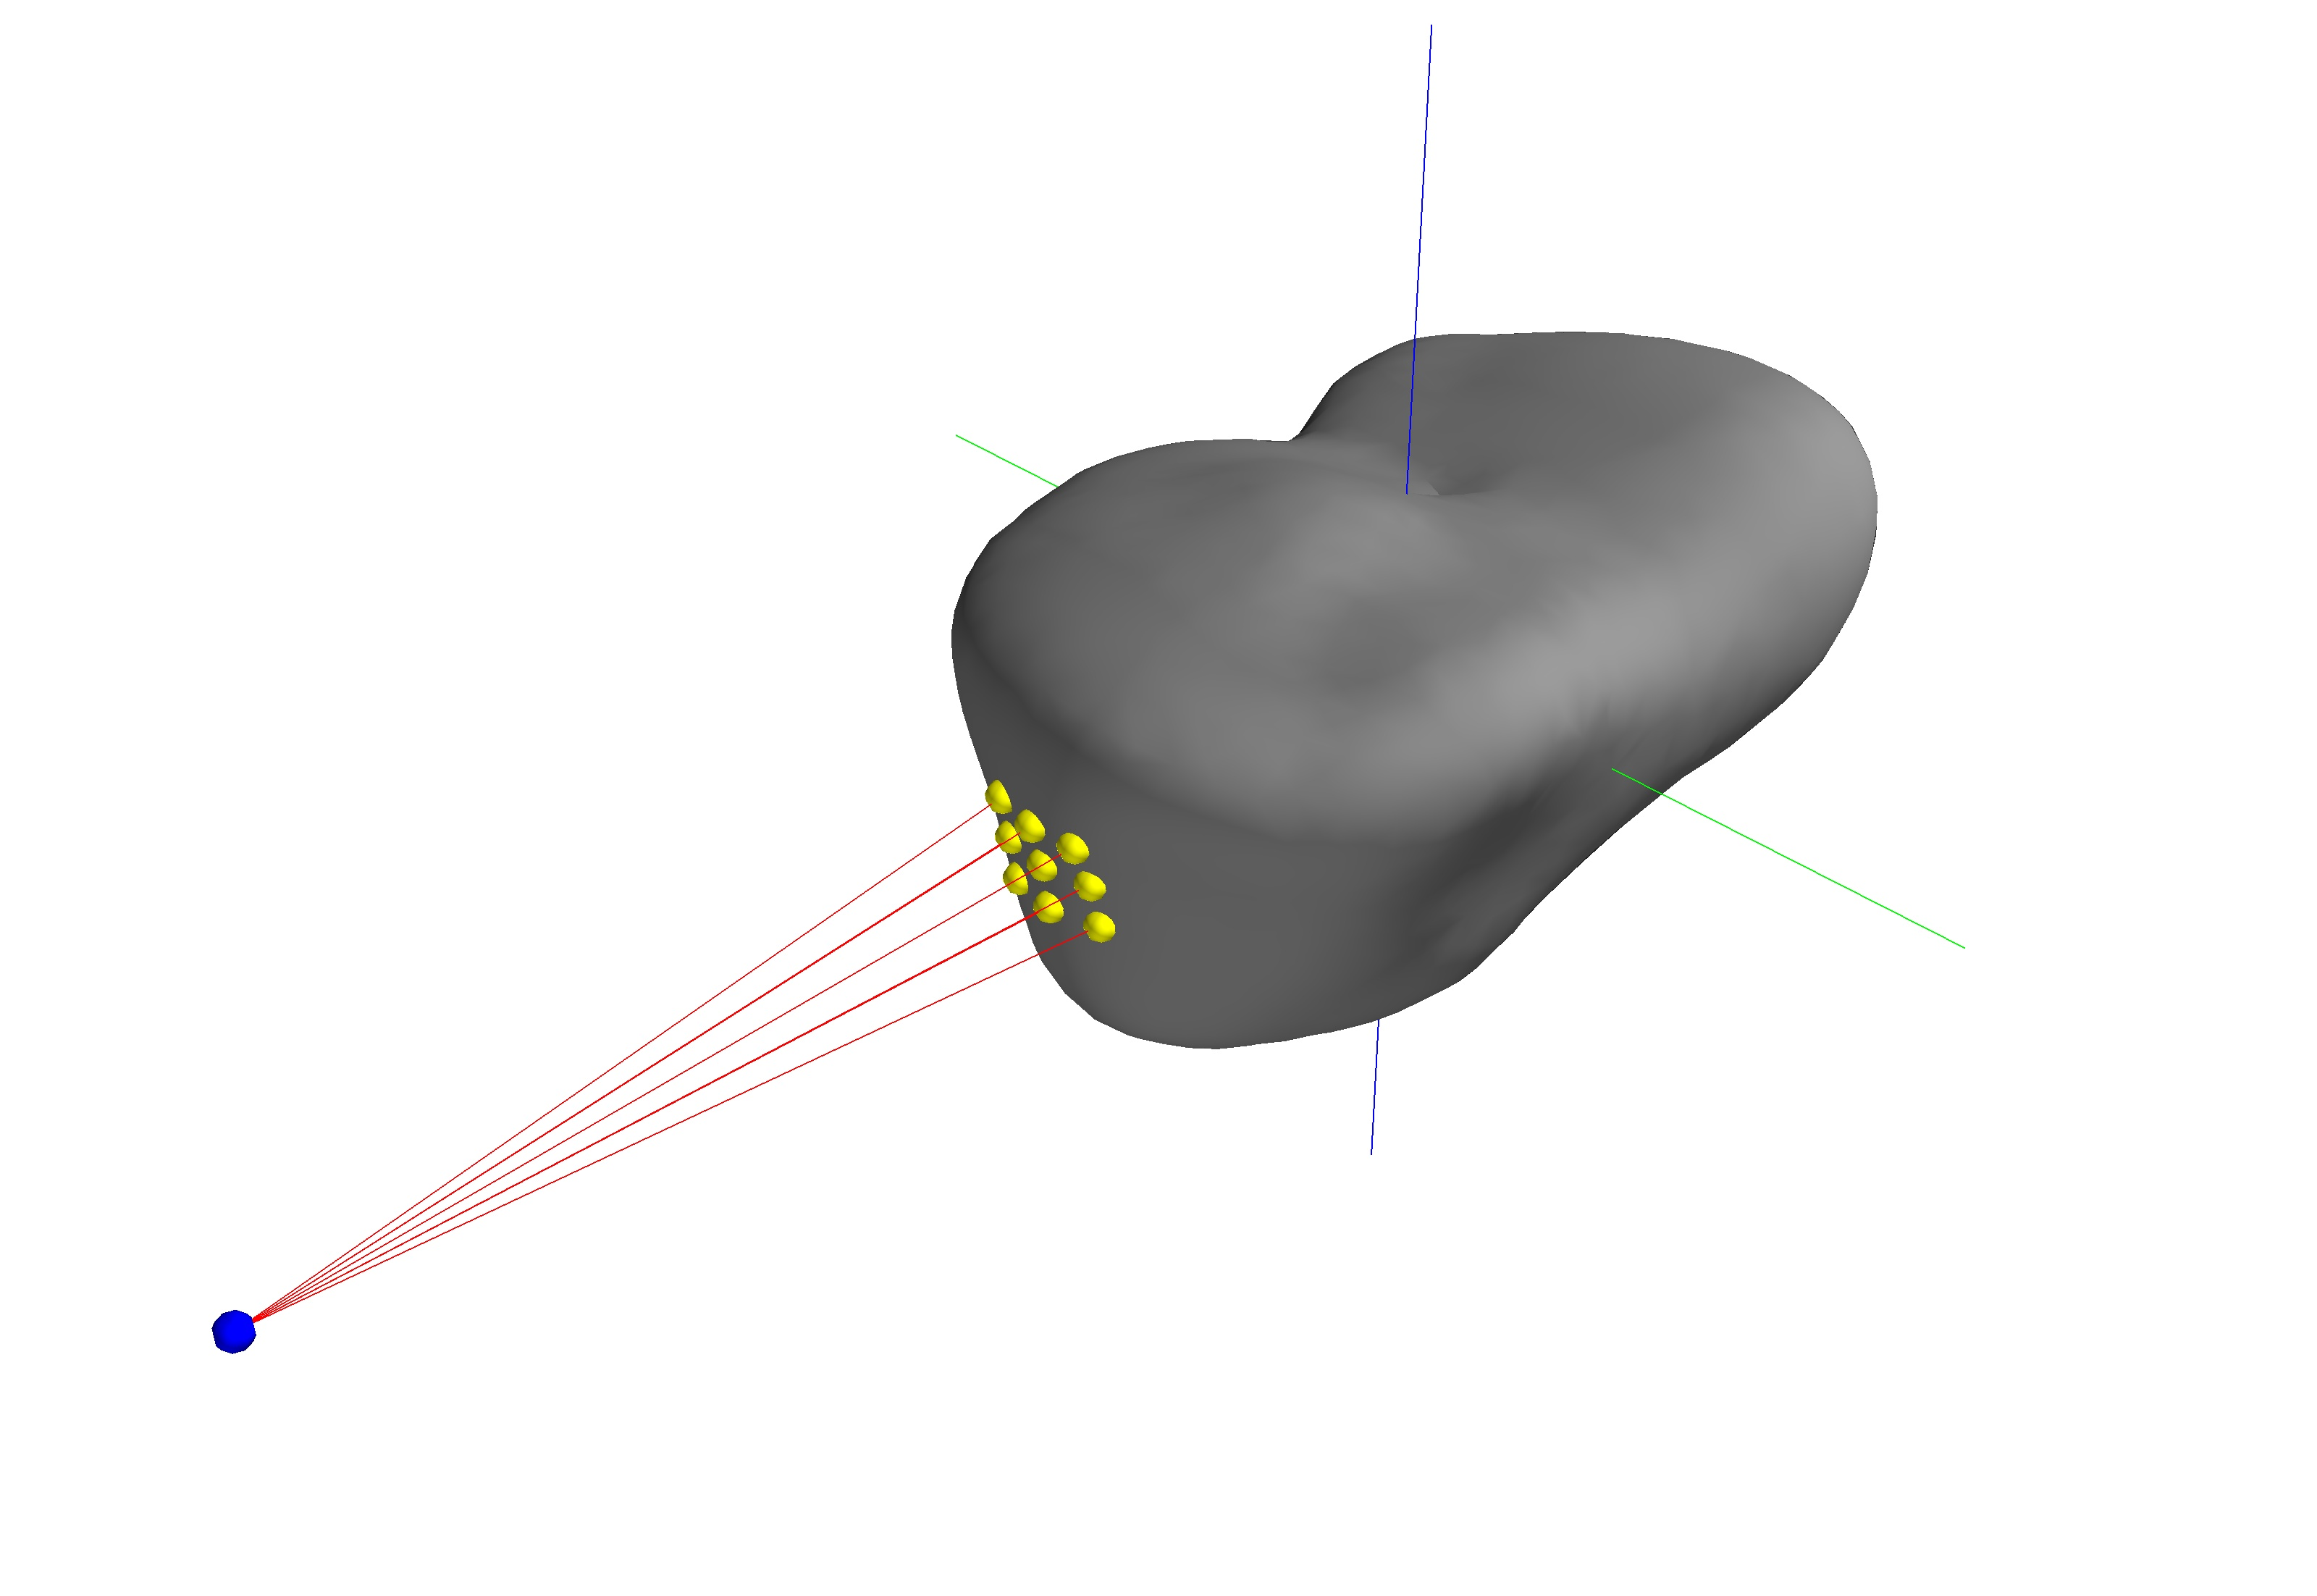
\includegraphics[width=0.75\textwidth]{figures/2018_SSPI/castalia_raycasting_plot.jpg}
    \caption{Simulated LIDAR measurements of asteroid Castalia~\label{fig:lidar_example}}
\end{figure}
We assume the spacecraft contains a range sensor, such as LIDAR, that allows for the accurate measurement of the relative distance between the spacecraft and asteroid~\cite{zuber1997,zuber2000}.
This type of sensor measures the round-trip time for a pulse of energy to leave the spacecraft, reflect off the surface, and return to a collector on board.
Given the time total time of flight, the distance can be accurately computed using \( d = \frac{\Delta TOF}{2 c} \) where \gls{sym:c} is the constant speed of light.
Assuming accurate knowledge of the pointing direction of the spacecraft we can compute a direction from the spacecraft to the measurement location on the surface.
The output of this sensor is a vector, \( \vc{d}_i \), defined in the spacecraft fixed frame which gives the direction to a measurement point on the surface of the asteroid. 
Using the state of the asteroid, we can transform this measurement to the asteroid fixed frame using the simple transformation
\begin{align*}
    \vb{p}_i = R_A^T R \vb{d}_i .
\end{align*}
Given many measurements, \( \vc{p}_i \), of the asteroid surface we can efficiently update our initial shape estimate to that of the true surface.
\Cref{fig:lidar_example} shows asteroid 4769 Castalia and a representation of several LIDAR measurements. 
The spacecraft measures the range between itself and the asteroid surface to several points within the field of view of the sensor. 
These measurements provide a collection of points which lie on the surface of the asteroid, and by combining many points, a so called ``point cloud'', allows us to reconstruct the shape.
% TODO Discuss point cloud reconstruction approaches (all computational exspensive and designed for unknown surfaces)

Our algorithm applies a Bayesian framework to radially modify each vertex \( \vc{v}_i \in \R^3\) of the shape estimate based on measurement \( \vc{p}_i \in \R^3 \). 
This approach alleviates much of complexity of incorporating new vertices or surface triangulation common in surface reconstruction methods~\cite{berg2008}.
This assumption means that the total number of vertices of the shape model is fixed.
However, additional detail, in the form of additional vertices, is possible by using standard mesh subdivision algorithms~\cite{orourke1998}, which we demonstrate in a subsequent section.

The radial distance of each vertex, \( v_i = \norm{\vc{v}_i}\), is assumed to be distributed according to the Gaussian distribution
\begin{align*}
    v_i \sim \mathcal{N}(r_i, w_i^2)
\end{align*}
where \( r_i \) is the initial estimate of the radial distance of vertex \( \vc{v}_i\) and \( w_i \) is the initial variance, or confidence, in the radial distance.
The radial distance of each measurement, \( p_{j,i} = \norm{\vc{p}_j}\), is also assumed to be distributed according to the Gaussian distribution
\begin{align*}
    p_{j,i} \sim \mathcal{N}(r_{j,i}, w_{j,i}^2)
\end{align*}
where \( r_{j,i} = \norm{\vc{p}_{j,i}} \) defines the radial distance of the surface vector measurement and \( w_{j, i}\) defines the variance of the measurement with respect to vertex \( \vc{v}_i\).
Each measurement is defined by the index \( j \) while the associated vertex is defined by \( i \). 
As a result, the measurement \( p_{j, i} \) defines the distribution of measurement \( j \) with respect to vertex \( i \). 
Any given measurement may be used to update one or several vertices.

The variance for each measurement vector is assumed to be related to the ``distance'' from the measurement to vertex \( \vc{v}_i \).
Here we use the \gls{geodesic} distance to parameterize the difference, and hence  uncertainty, of associating the measurement with a given vertex.
From spherical trigonometry~\cite{gade2010} the central angle between measurement \( \vc{p}_i \) and vertex \( \vc{v}_i \) of the shape estimate is
\begin{align}\label{eq:geodesic_distance}
    \Delta \sigma_{j,i} = \arctan \parenth{\frac{\norm{\vc{p}_j \times \vc{v}_i}}{\vc{p}_j \cdot \vc{v}_i }}.
\end{align}
The variance of measurement \( \vc{p}_i \) with respect to vertex \( \vc{v}_i \) is then defined as the arc length as
\begin{align}
    w_{j, i} = \norm{\vc{p}_j} \Delta \sigma_{j,i} .
\end{align}
This approach relates the uncertainty of the measurement, \( \vb{p}_j \) with the geodesic distance to a given vertex, \( \vb{v}_i \).
As a result, measurements which are far from a vertex, where \( \Delta \sigma \) is large, will tend to have a larger variance and hence uncertainty. 
This approach can be considered as a form of a correlation based sensor model~\cite{thrun2005}.
The main benefit of a correlation based approach, in constrast to feature extraction is the relative simplicity of implementation.
However, the resulting correlation values do not posses any physical significance and do not represent the noise or uncertainty characteristics of the sensor.

From Bayes' theorem, the posterior probability is
\begin{align}
    p(v_i | p_{j, i}) = \frac{p(p_{j, i} | v_i) p(v_i)}{p( p_{j, i})} \propto p(p_{j,i} | v_i) p(v_i).
\end{align}
From the properties of a Gaussian, the posterior probability given a measurement is also distributed according to a Gaussian distribution~\cite{bishop2006} and given by
\begin{align}\label{eq:posterior_probability}
    \mathcal{N} \parenth{\frac{w_{j, i}^2 r_i + w_i^2 r_{j, i}}{w_i^2 + w_{j, i}^2} , \frac{w_i^2  w_{j, i}^2}{w_i^2 +  w_{j, i}^2}} .
\end{align}
From~\cref{eq:posterior_probability}, the posterior probability conditioned on the measurement is the weighted average of the prior knowledge and the measurement. 
Measurements that are far from the vertex will have a high uncertainty or variance and will have a reduced impact on the radial position of the vertex.
Additional measurements are incorporated using a weighted average of prior belief and the measurement uncertainty.

In order to improve the computational efficiency measurement updates are assumed to be local in nature.
Instead of applying a measurement to all vertices of the mesh, the measurement is only applied to the vertices which are within a specified region of the measurement. 
We define a region of interest, \( \Delta S \), about each measurement which defines the surface area over which the measurement will affect the mesh estimate.
We relate \( \Delta S \) to an equivalent angular constraint using
\begin{align}\label{eq:region_of_interest}
    \Delta \sigma_{max} = \sqrt \frac{\Delta S}{r_b^2}
\end{align}
where \( r_b \) defines the Brillouin  sphere radius, or the radius of the circumscribing sphere of the asteroid.
Only vertices which satisfy \( \Delta \sigma_i \leq \Delta \sigma_{max} \) are considered in the Bayesian update shown in~\cref{eq:posterior_probability}.

The approach presented in~\cref{sec:radius_update} allows one to update the shape of an asteroid given a single range measurement of the surface.
A sequential process can be used to iteratively update the shape estimate given many measurements of the surface. 
For example,~\cref{fig:reconstruction} illustrates the process of updating an initial shape estimate of asteroid 4769 Castalia.
The initial shape for Castalia is a triaxial ellipsoid with semi-axes equal to \( \SI{1.8}{\kilo\meter} \times \SI{0.8}{\kilo\meter} \times \SI{0.8}{\kilo\meter}\) and shown in~\cref{fig:start}.

Simulated measurements of the surface of 4769 Castalia are used to update the initial mesh estimate.
The truth shape model, and the associated vertices, are used as simulated measurements of the shape of Castalia~\cite{neese2004}.
The true shape model of 4769 Castalia is composed of \num{2048} vertices and \num{4092} triangular faces.
The initial shape estimate is chosen to have approximately the same number of vertices as the final true shape and such that the total number of vertices remains constant.
\begin{figure}[htbp]
    \centering
    \subcaptionbox{Initial mesh estimate\label{fig:start}}{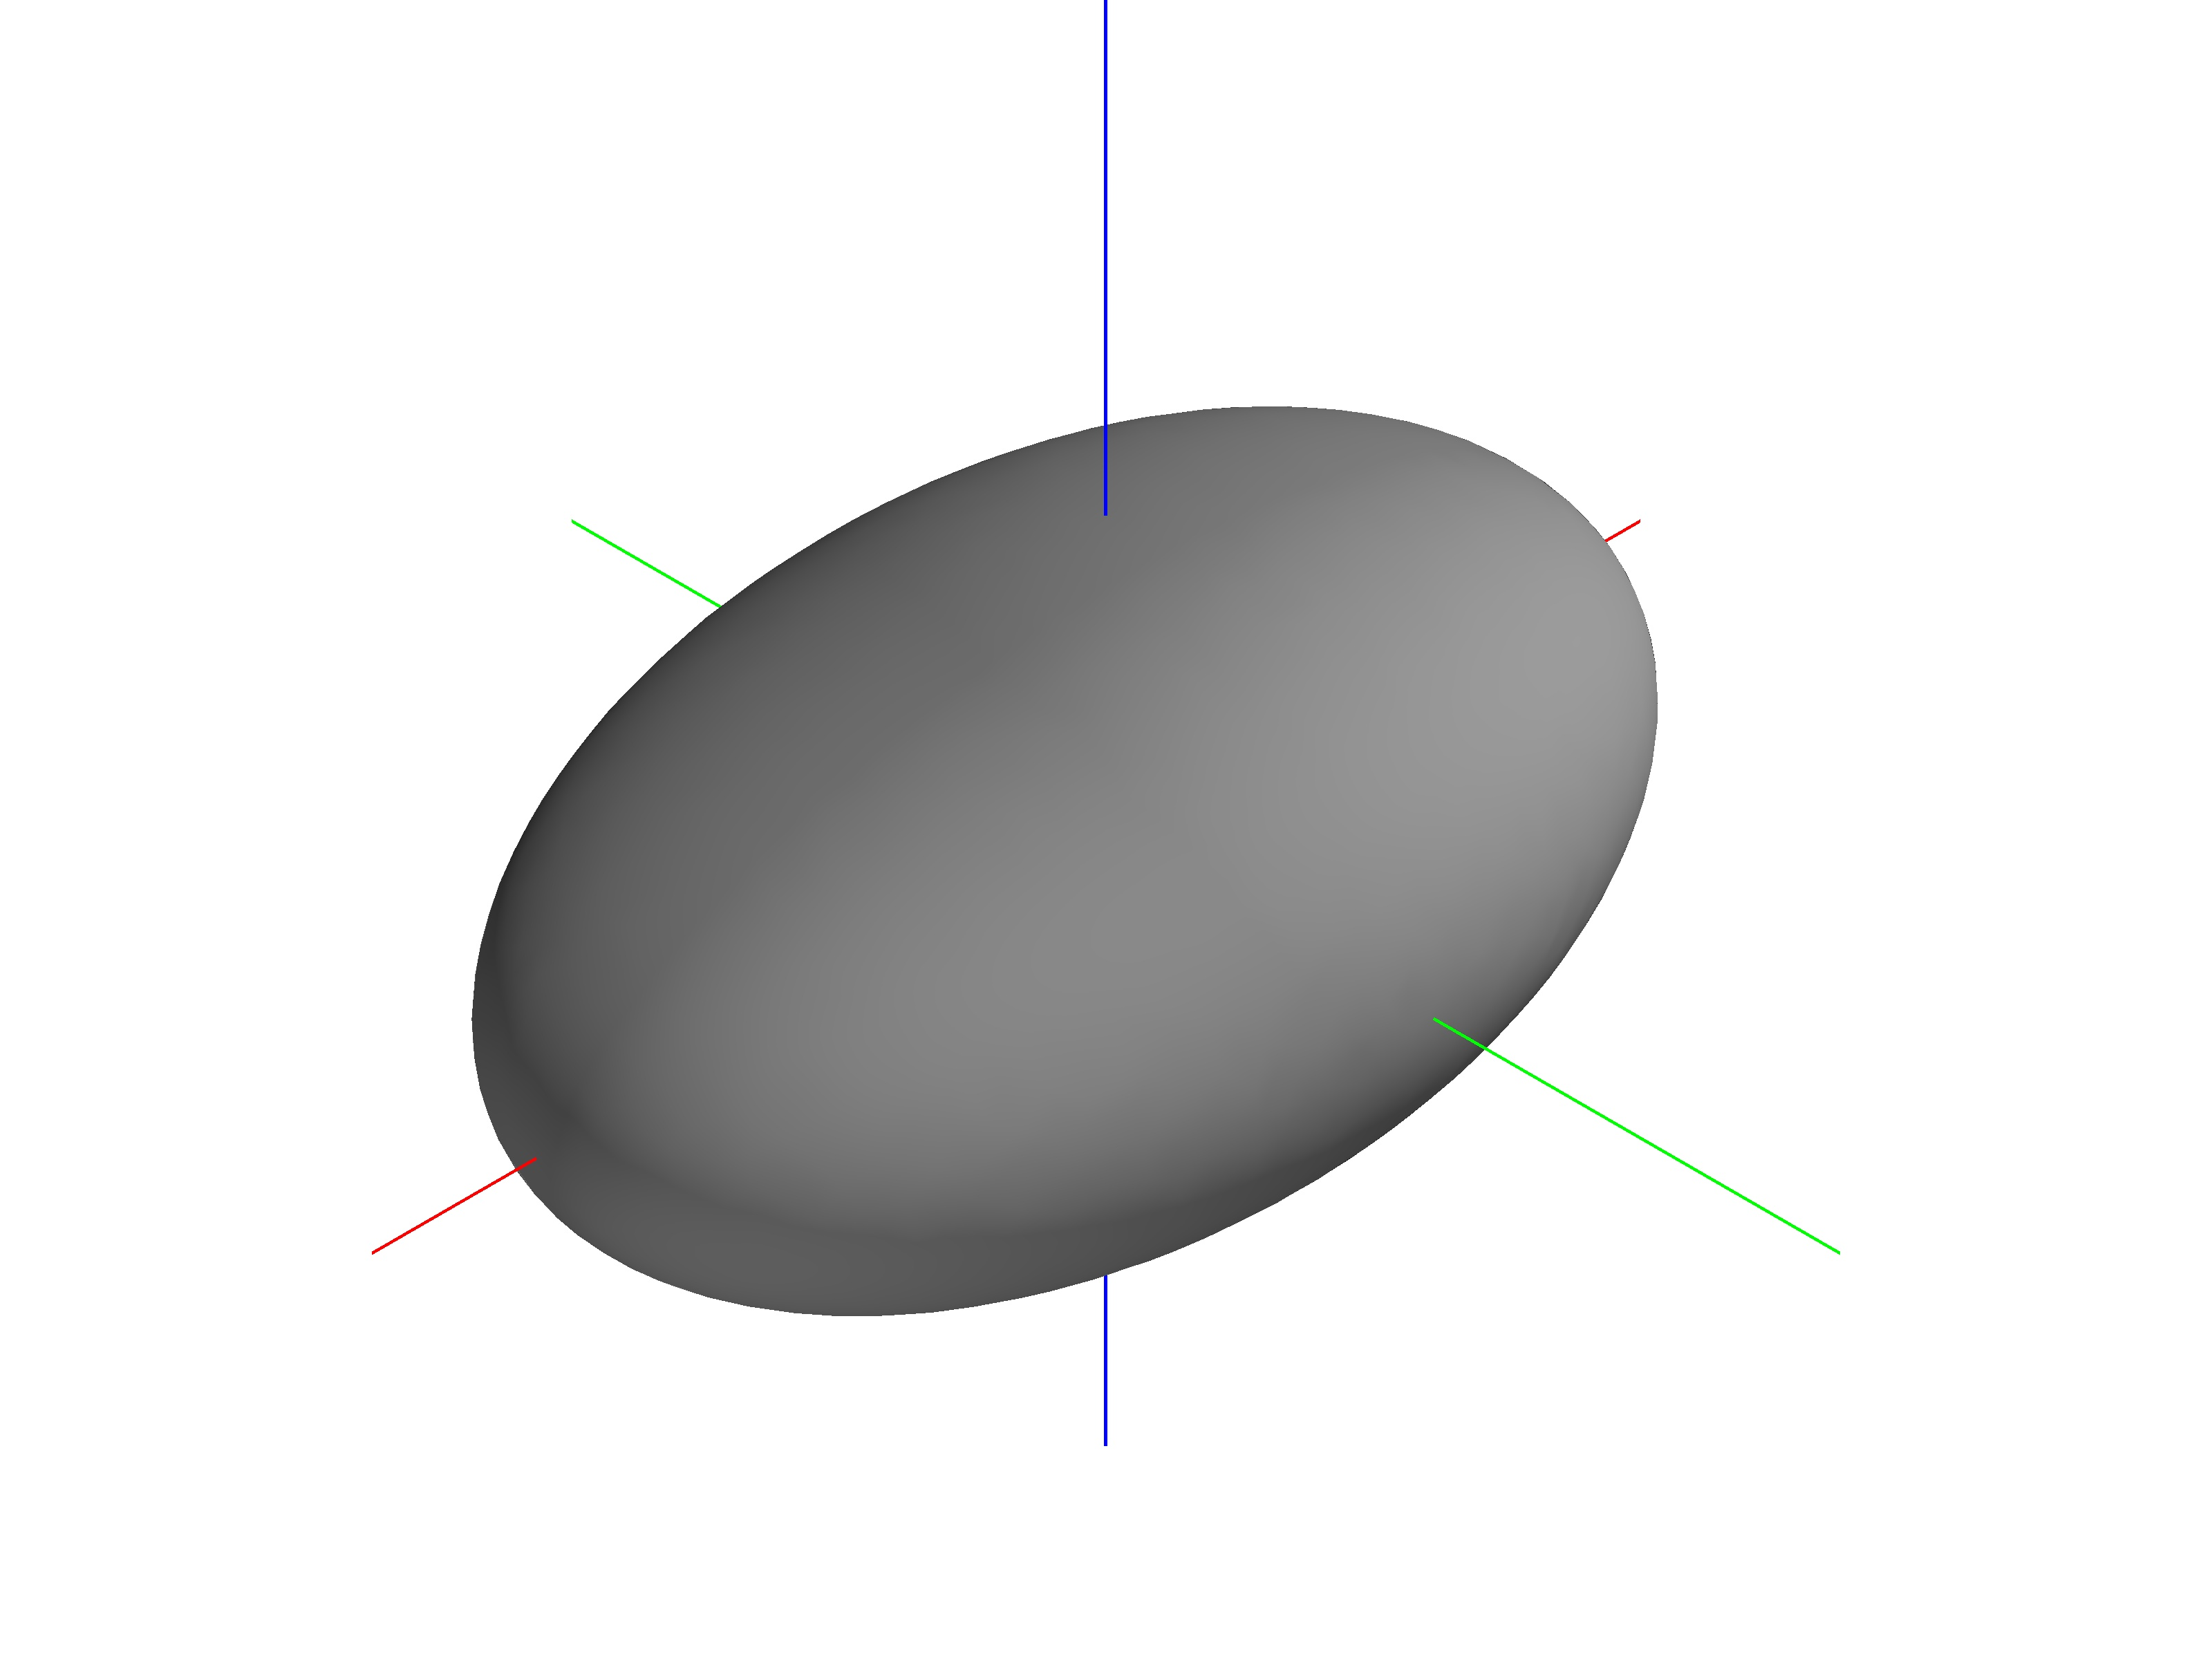
\includegraphics[height=0.5\textheight,width=0.5\textwidth,keepaspectratio]{figures/2018_SSPI/partial_initial.jpg}}~
    \subcaptionbox{First measurement added\label{fig:first}}{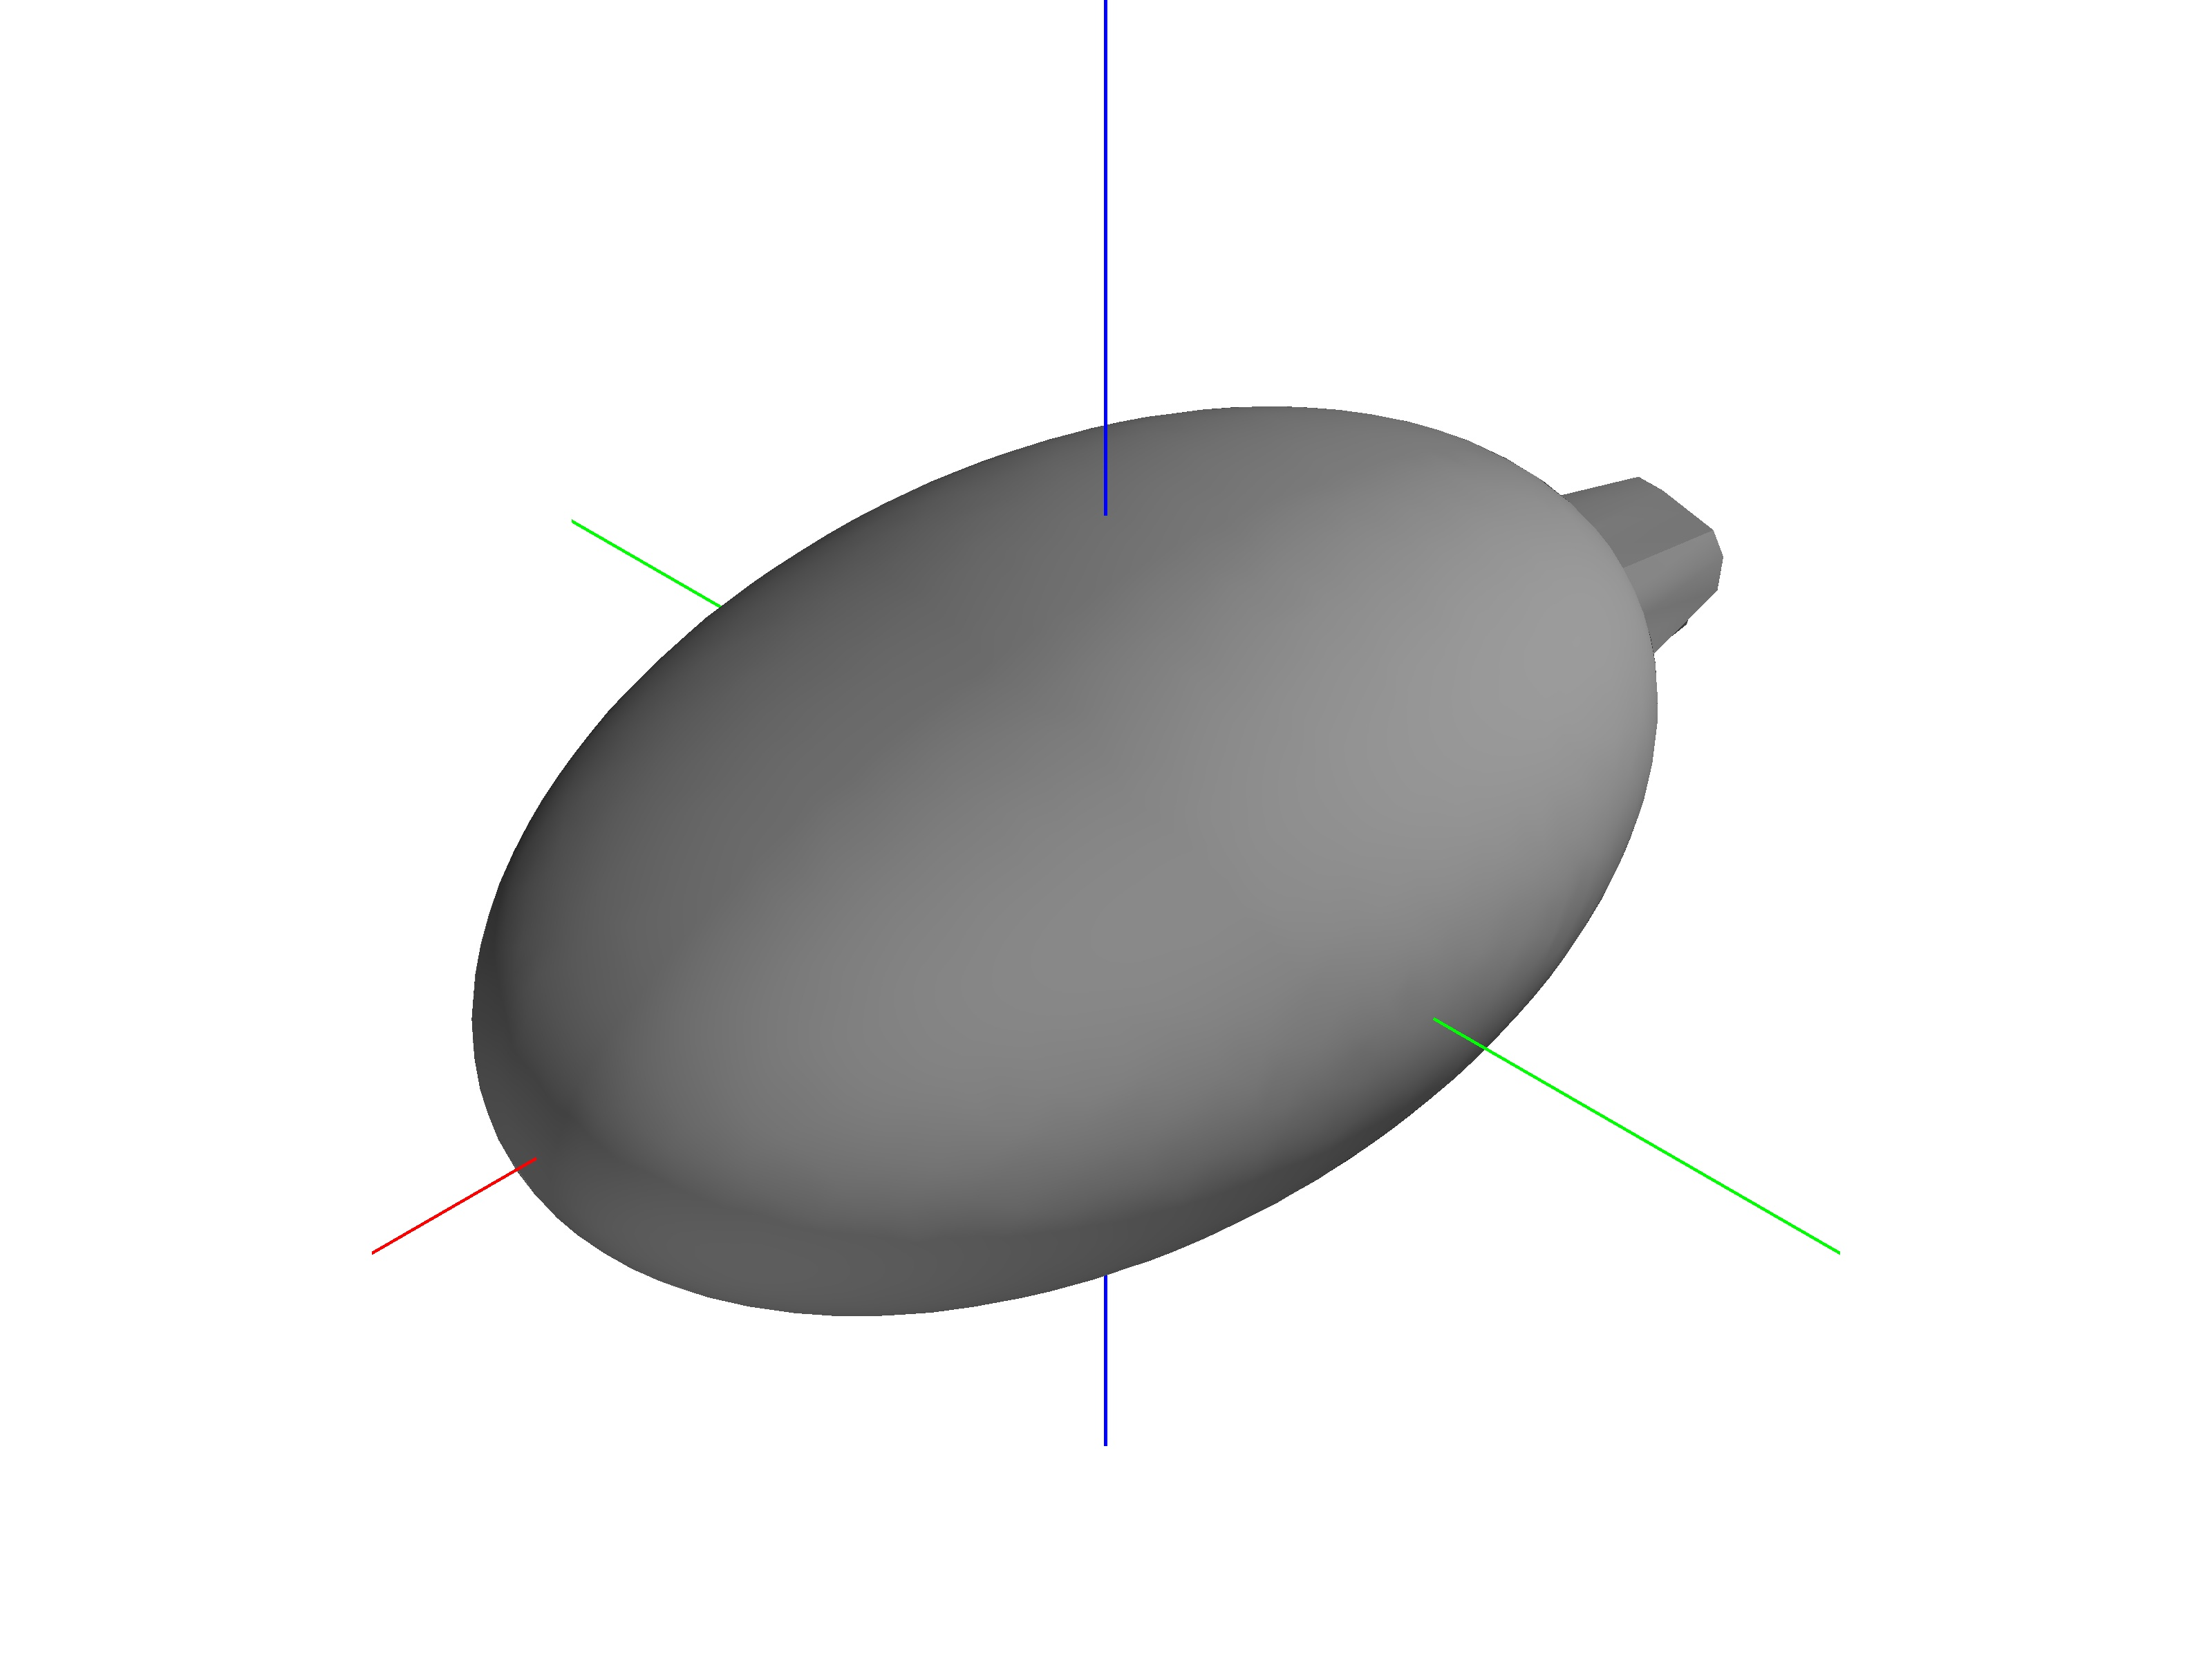
\includegraphics[width=0.5\textwidth]{figures/2018_SSPI/partial_0.jpg}}

    \subcaptionbox{\SI{25}{\percent} of measurments added\label{fig:quarter}}{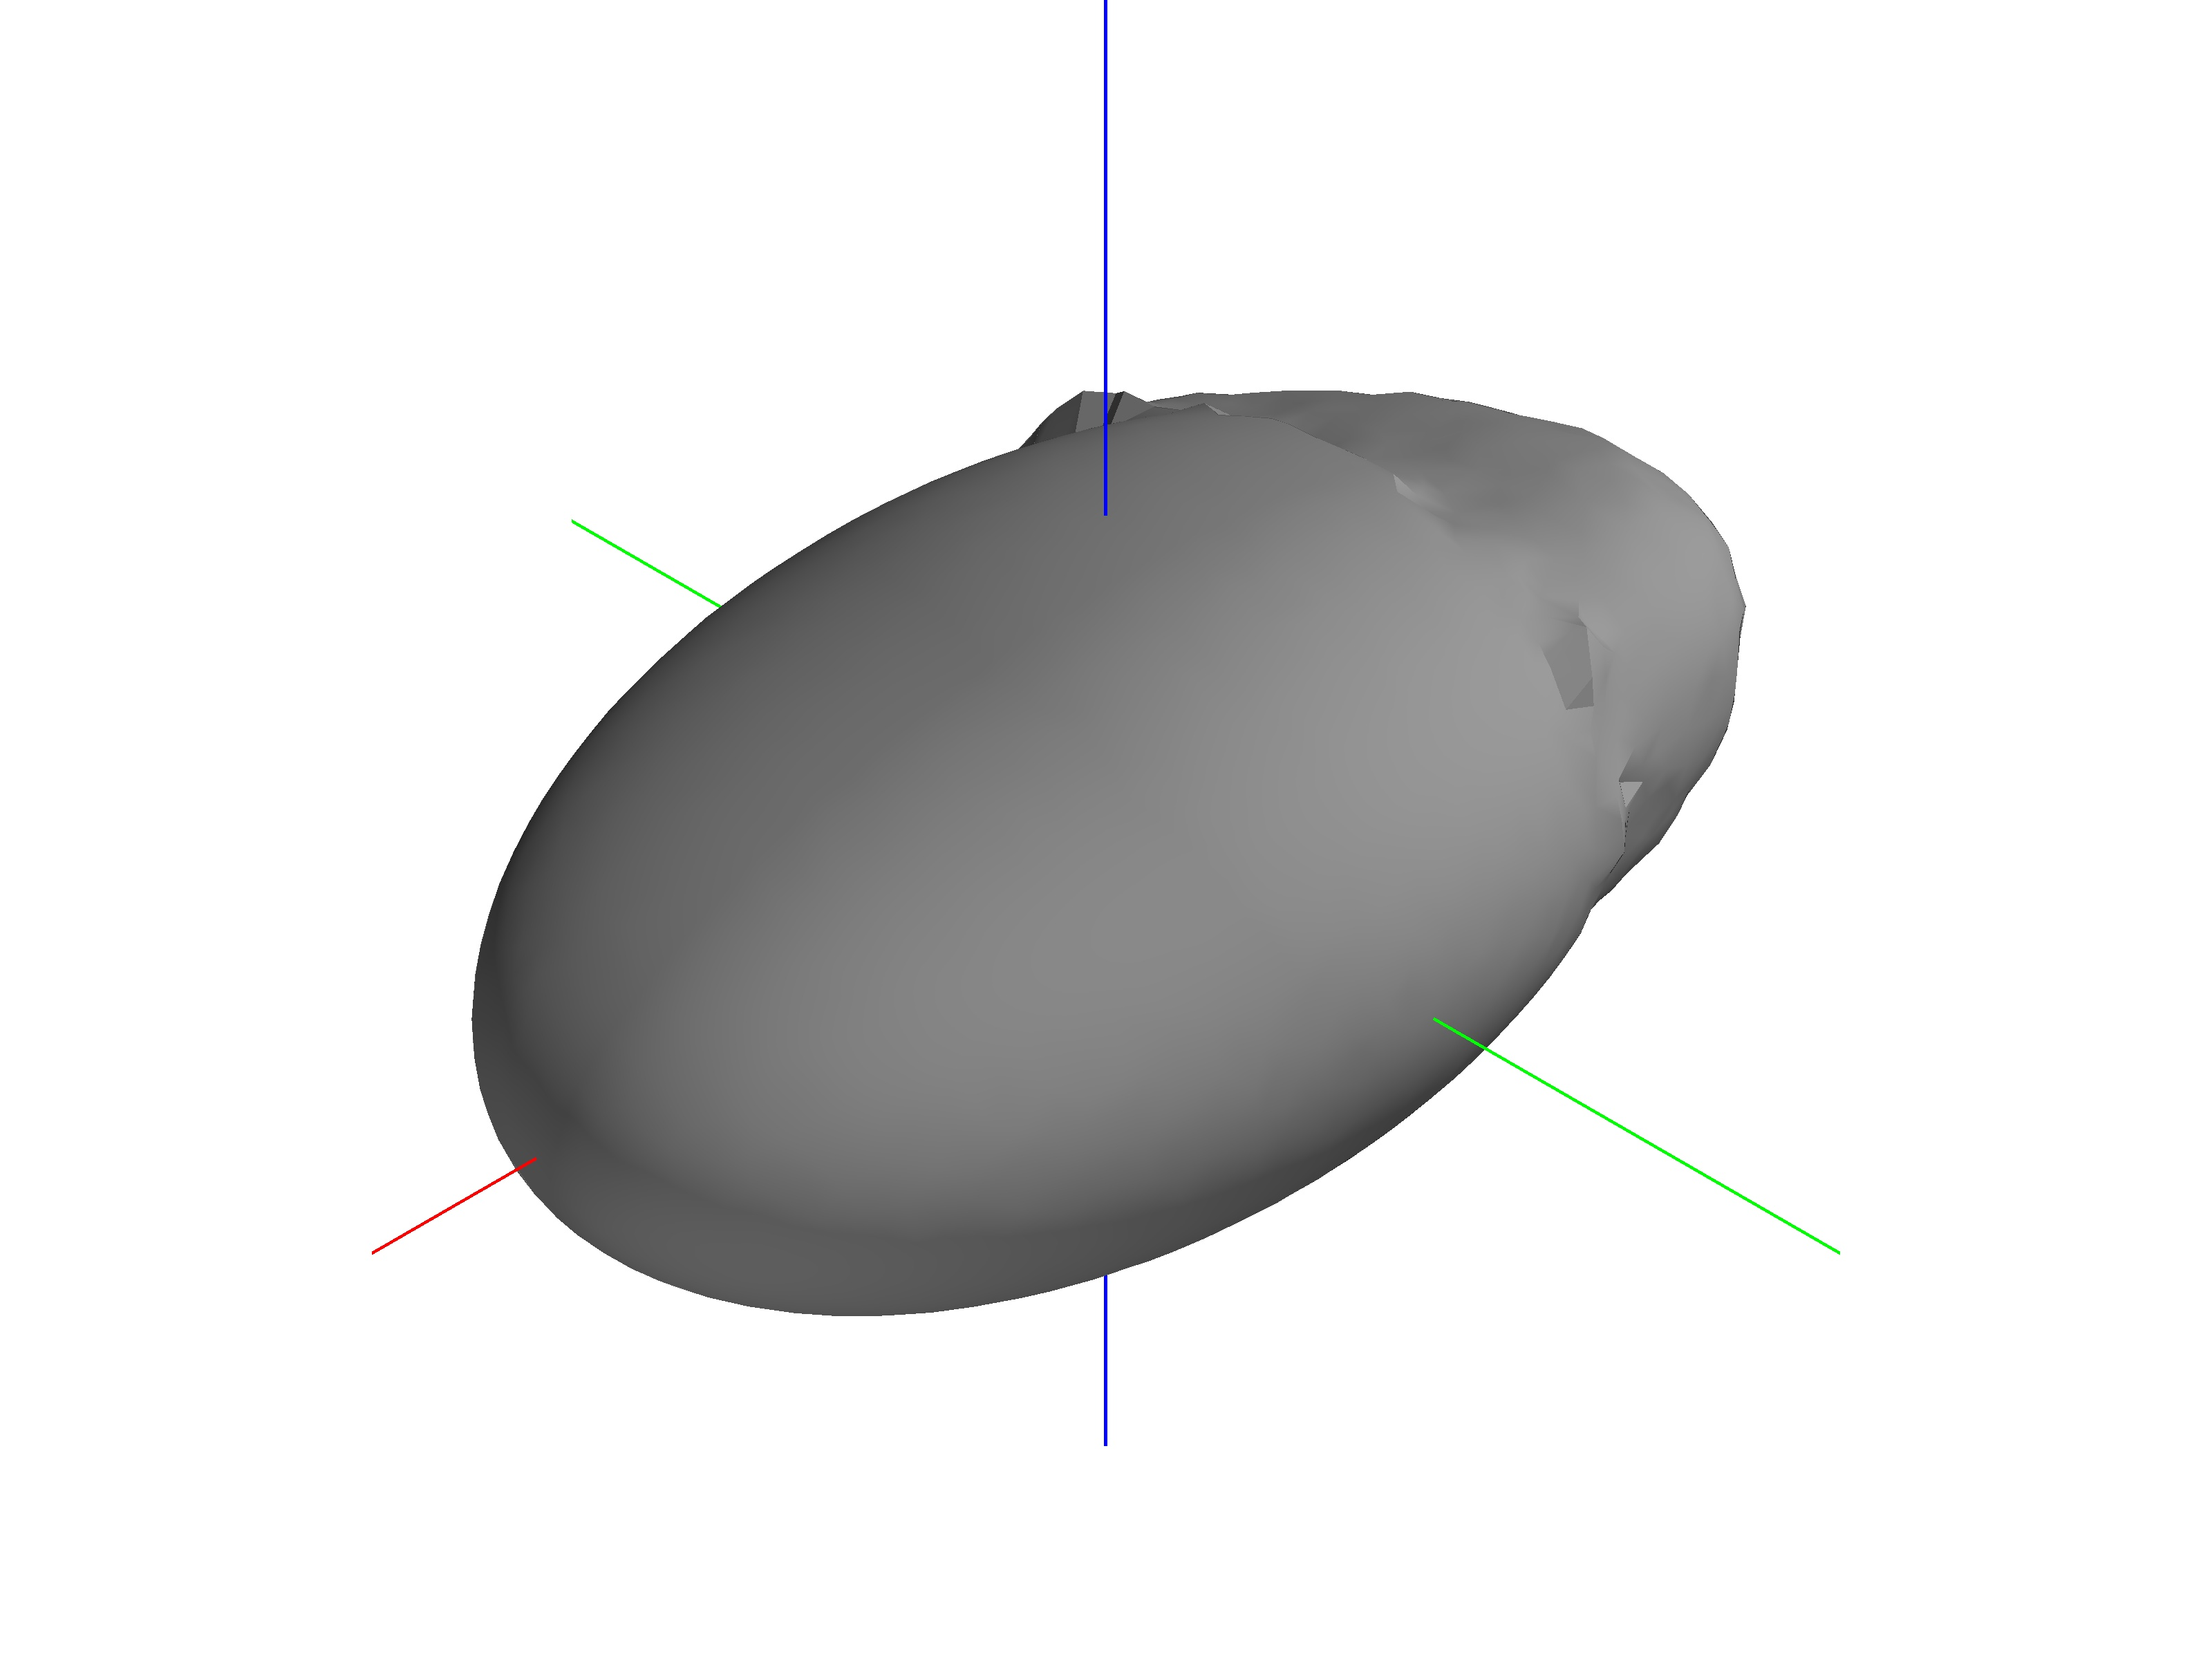
\includegraphics[width=0.5\textwidth]{figures/2018_SSPI/partial_512.jpg}}~
    \subcaptionbox{\SI{50}{\percent} of measurements added\label{fig:half}}{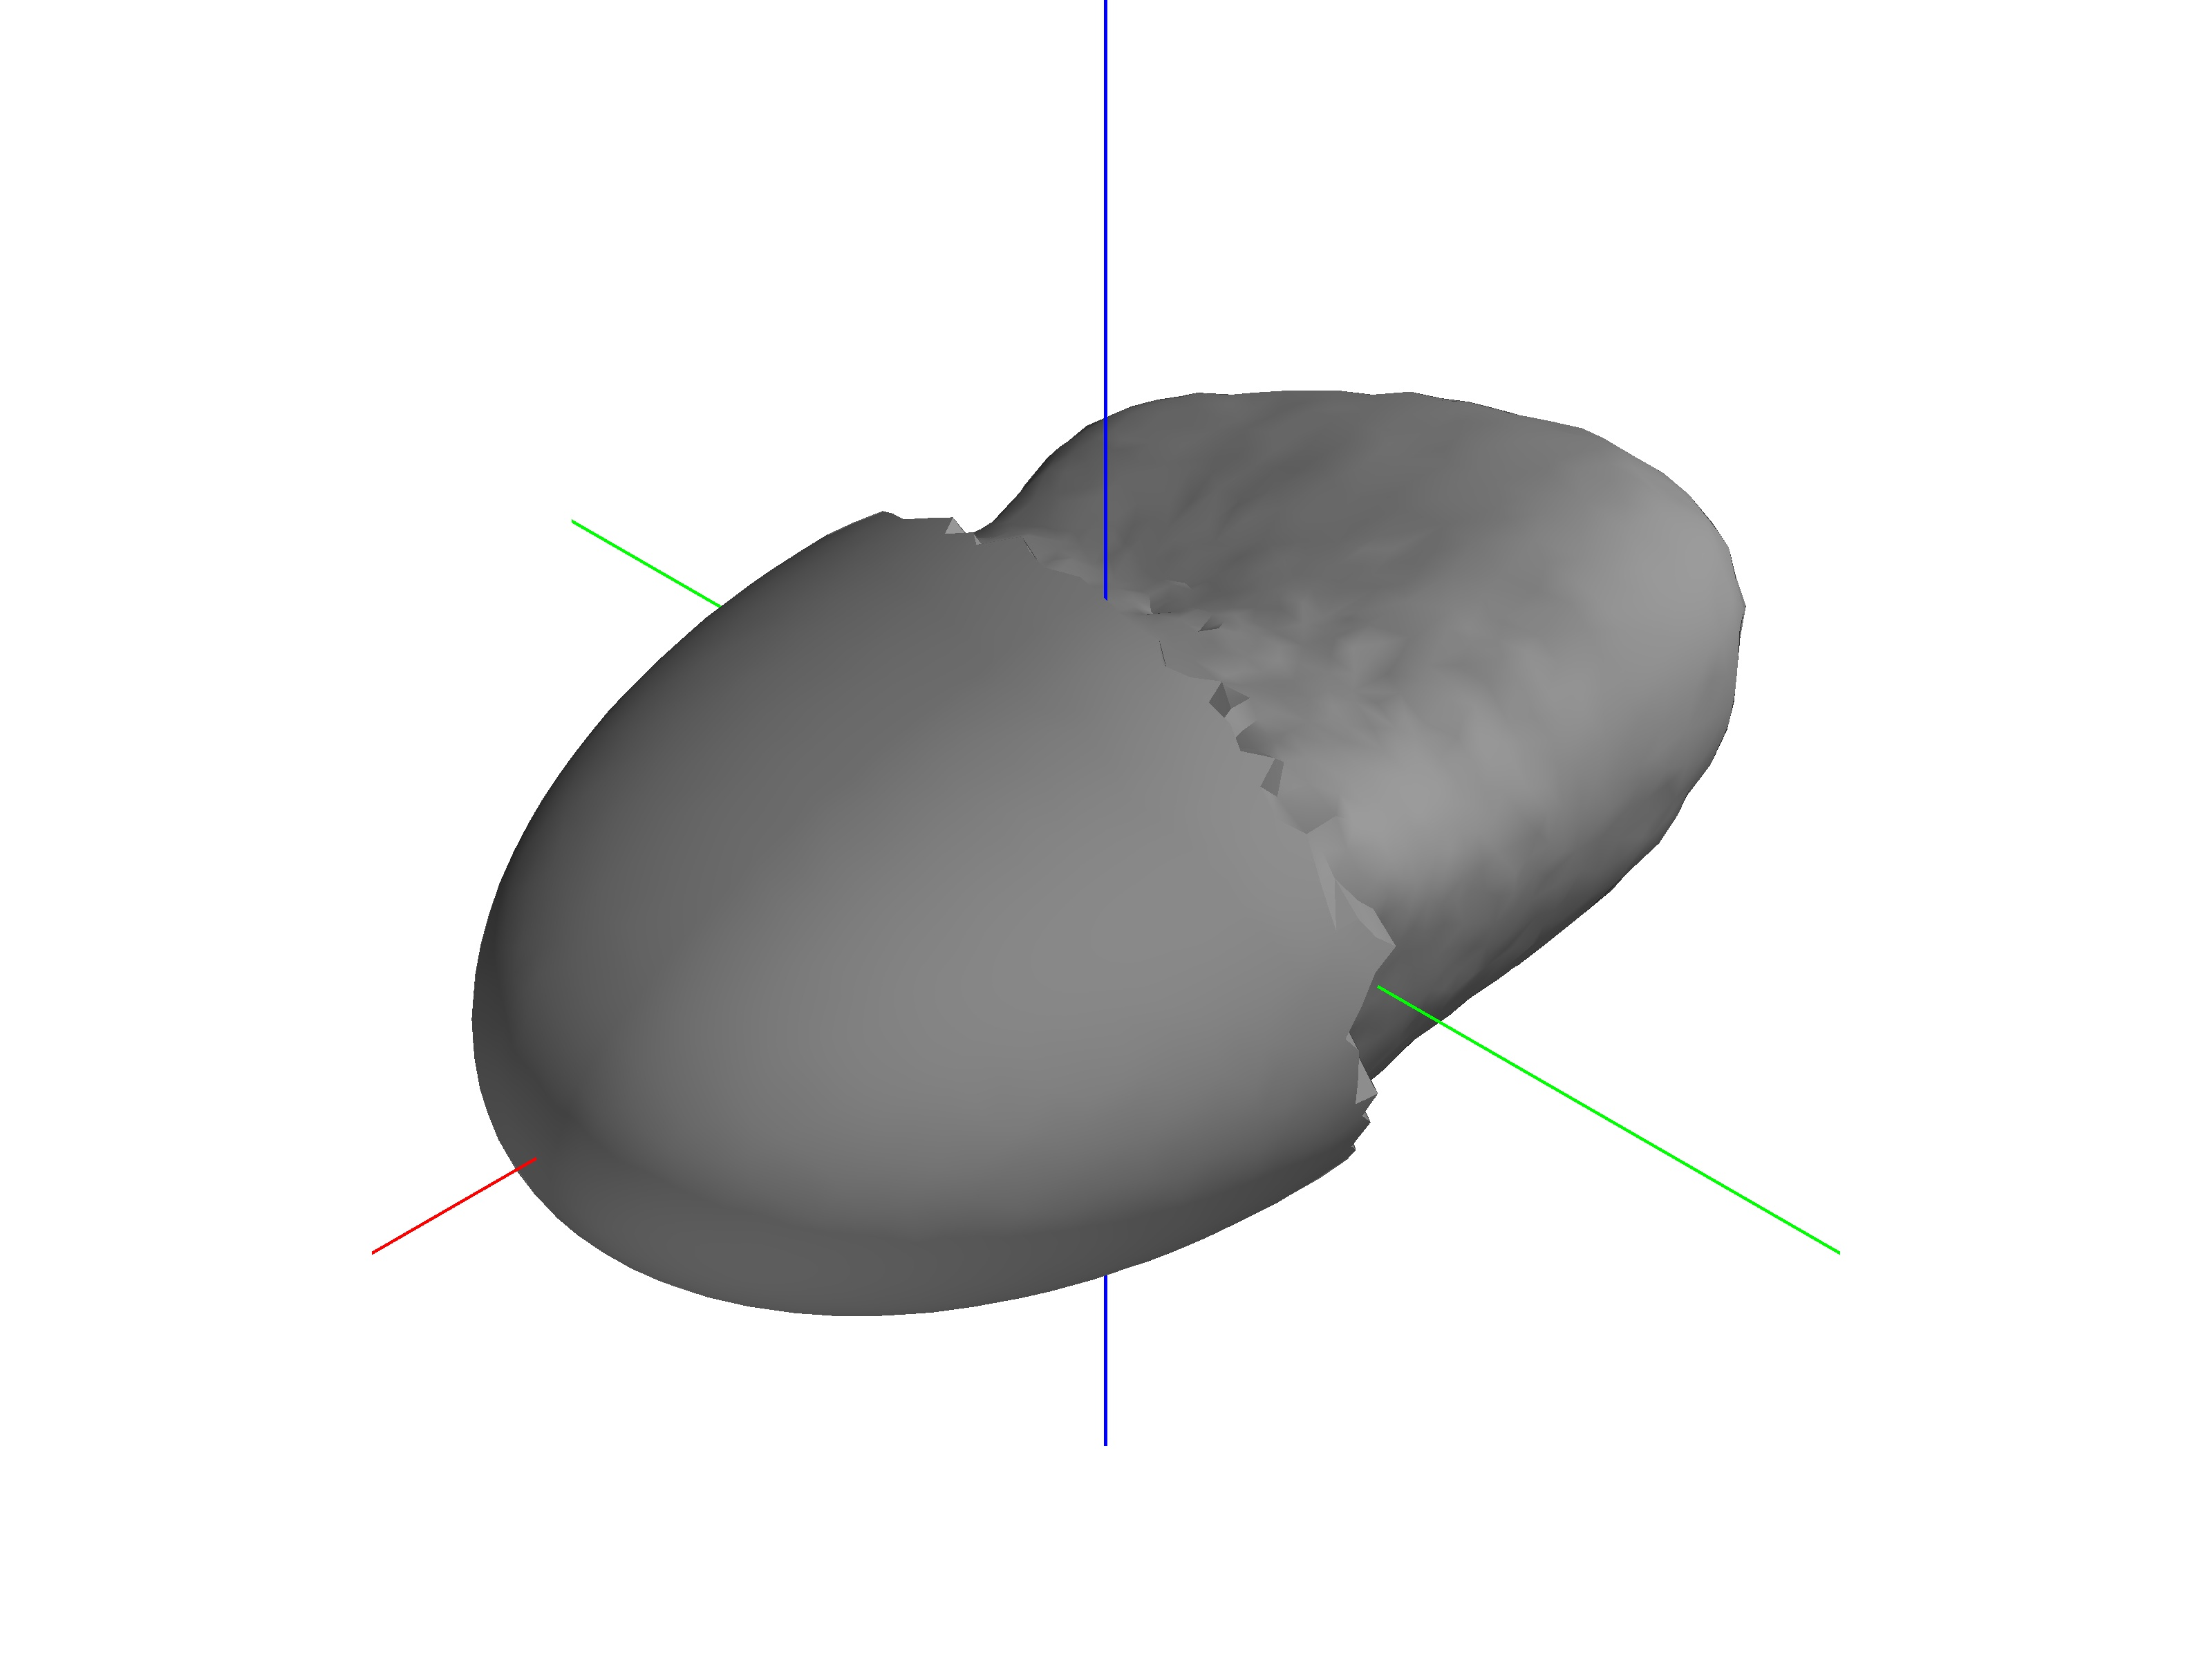
\includegraphics[width=0.5\textwidth]{figures/2018_SSPI/partial_1024.jpg}}

    \subcaptionbox{\SI{75}{\percent} of measurements added\label{fig:threequarter}}{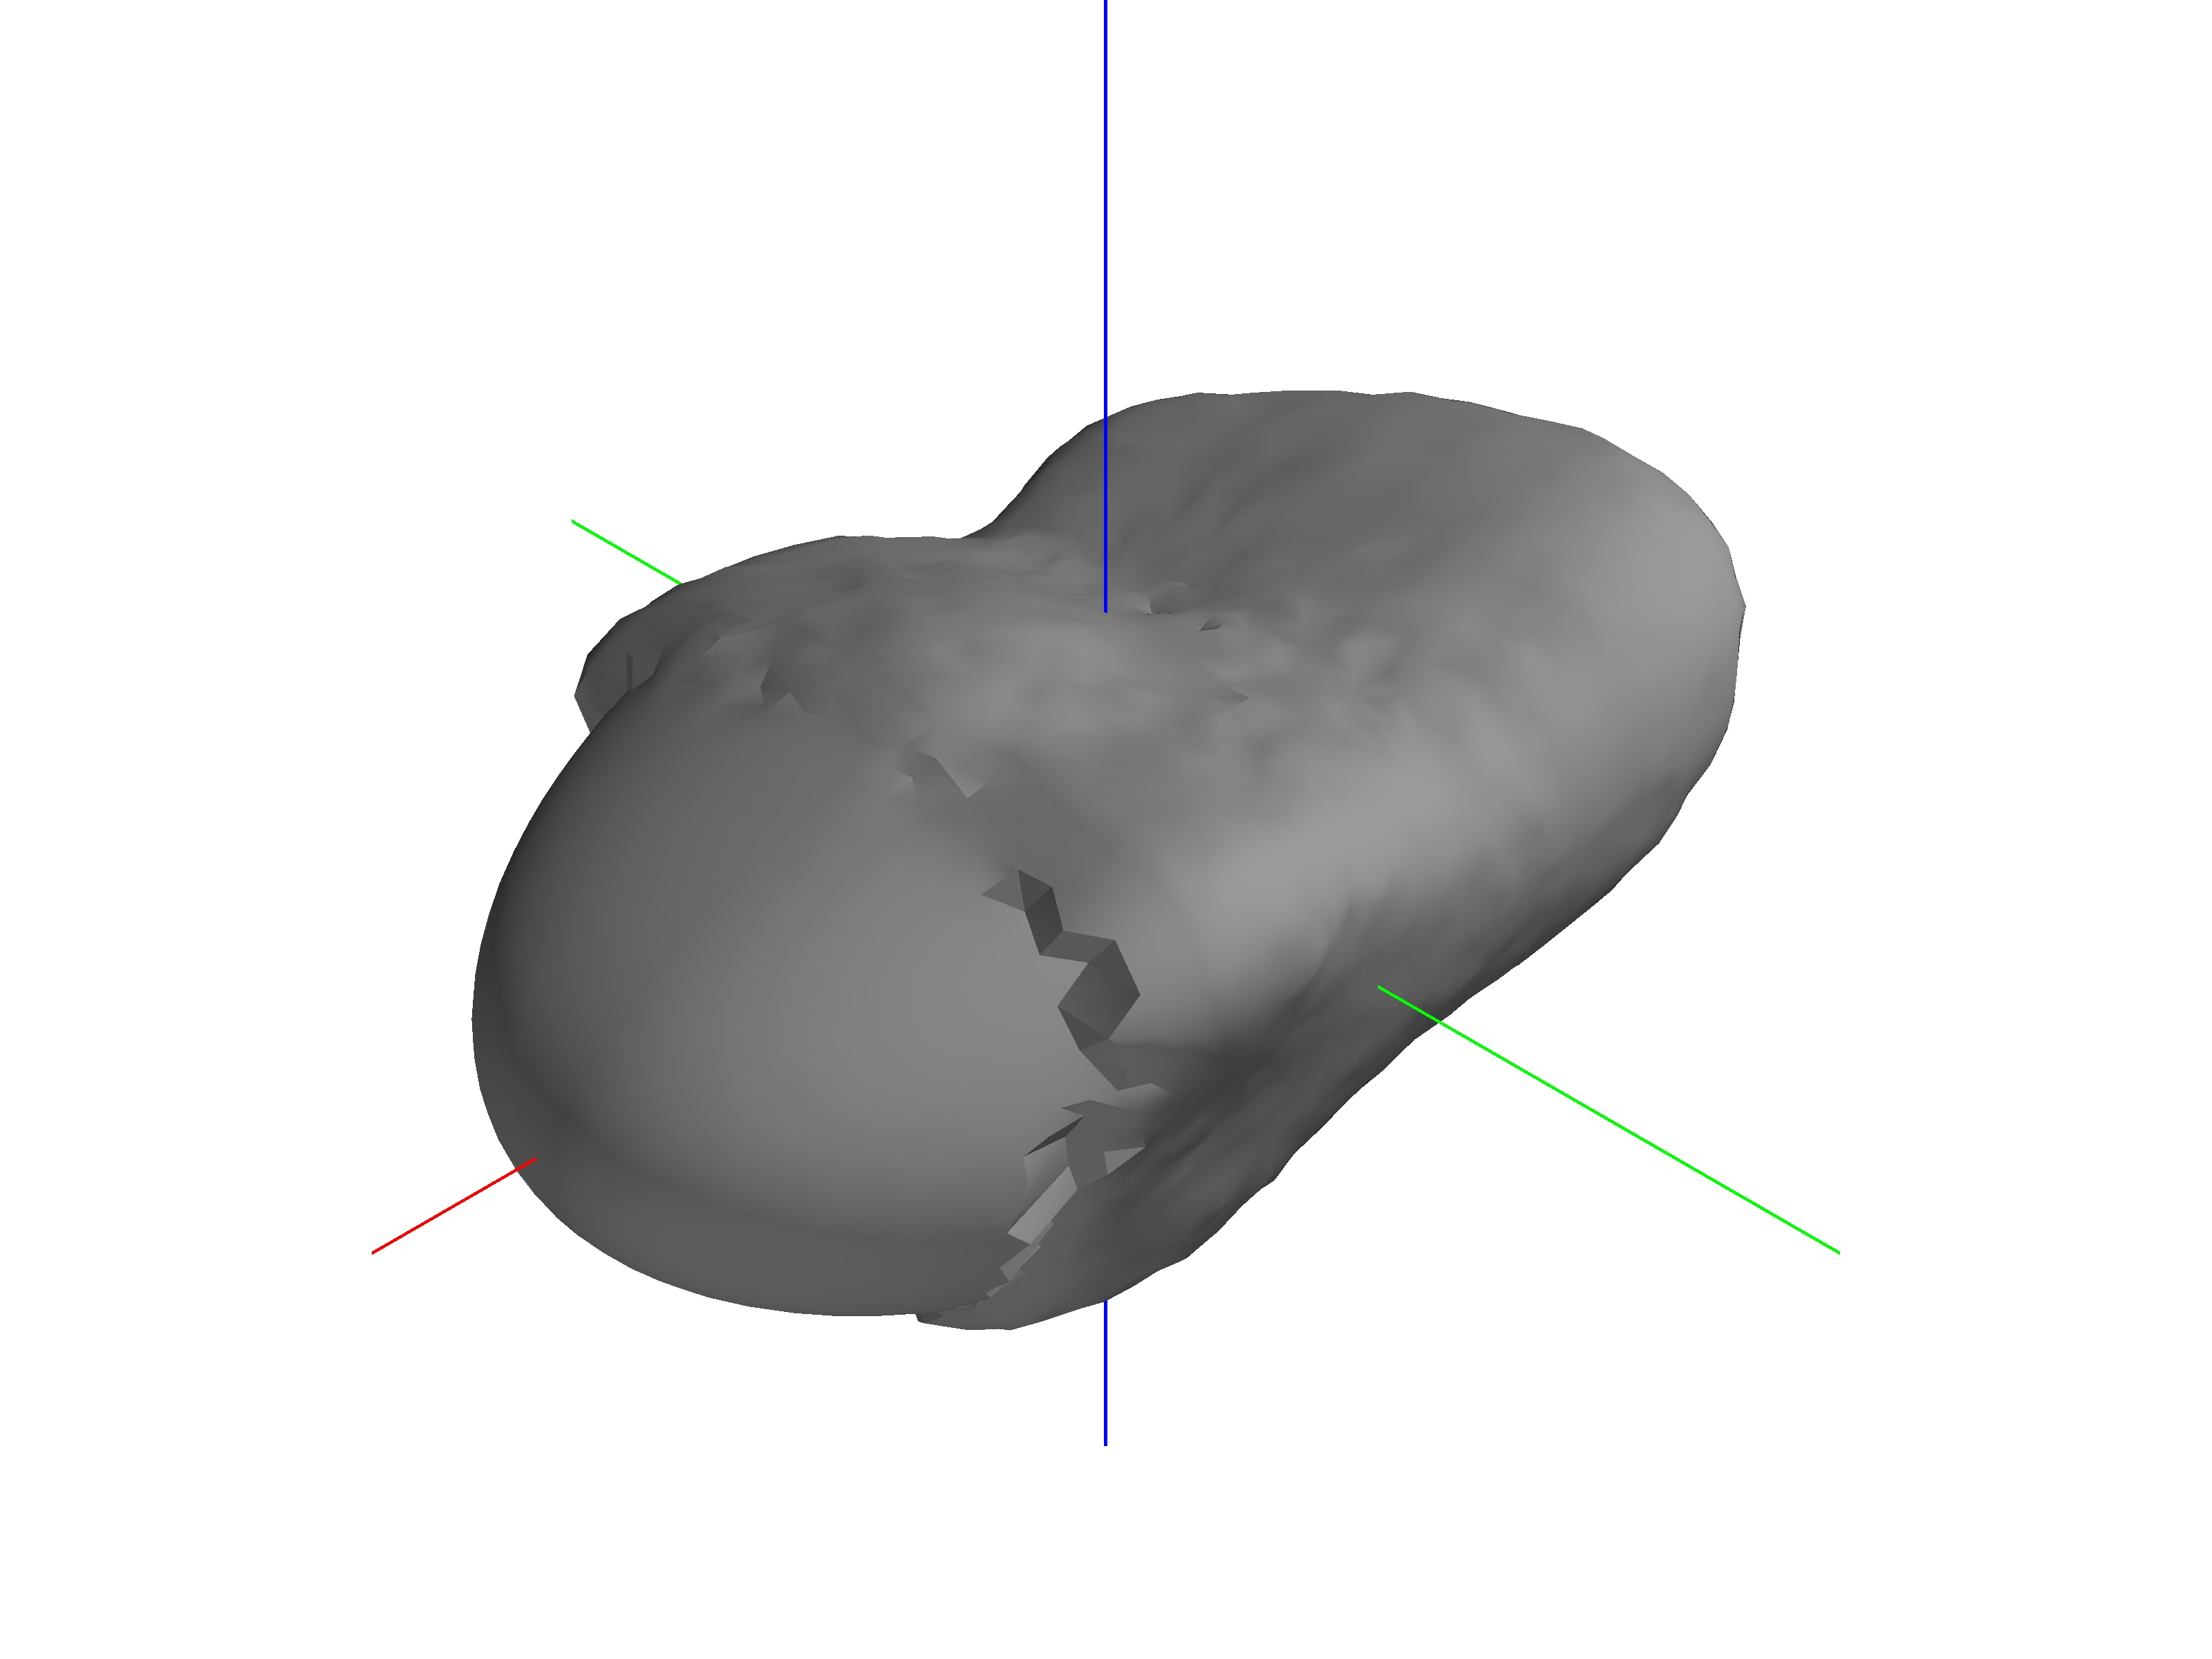
\includegraphics[width=0.5\textwidth]{figures/2018_SSPI/partial_1536.jpg}}~
    \subcaptionbox{Final reconstruction\label{fig:final}}{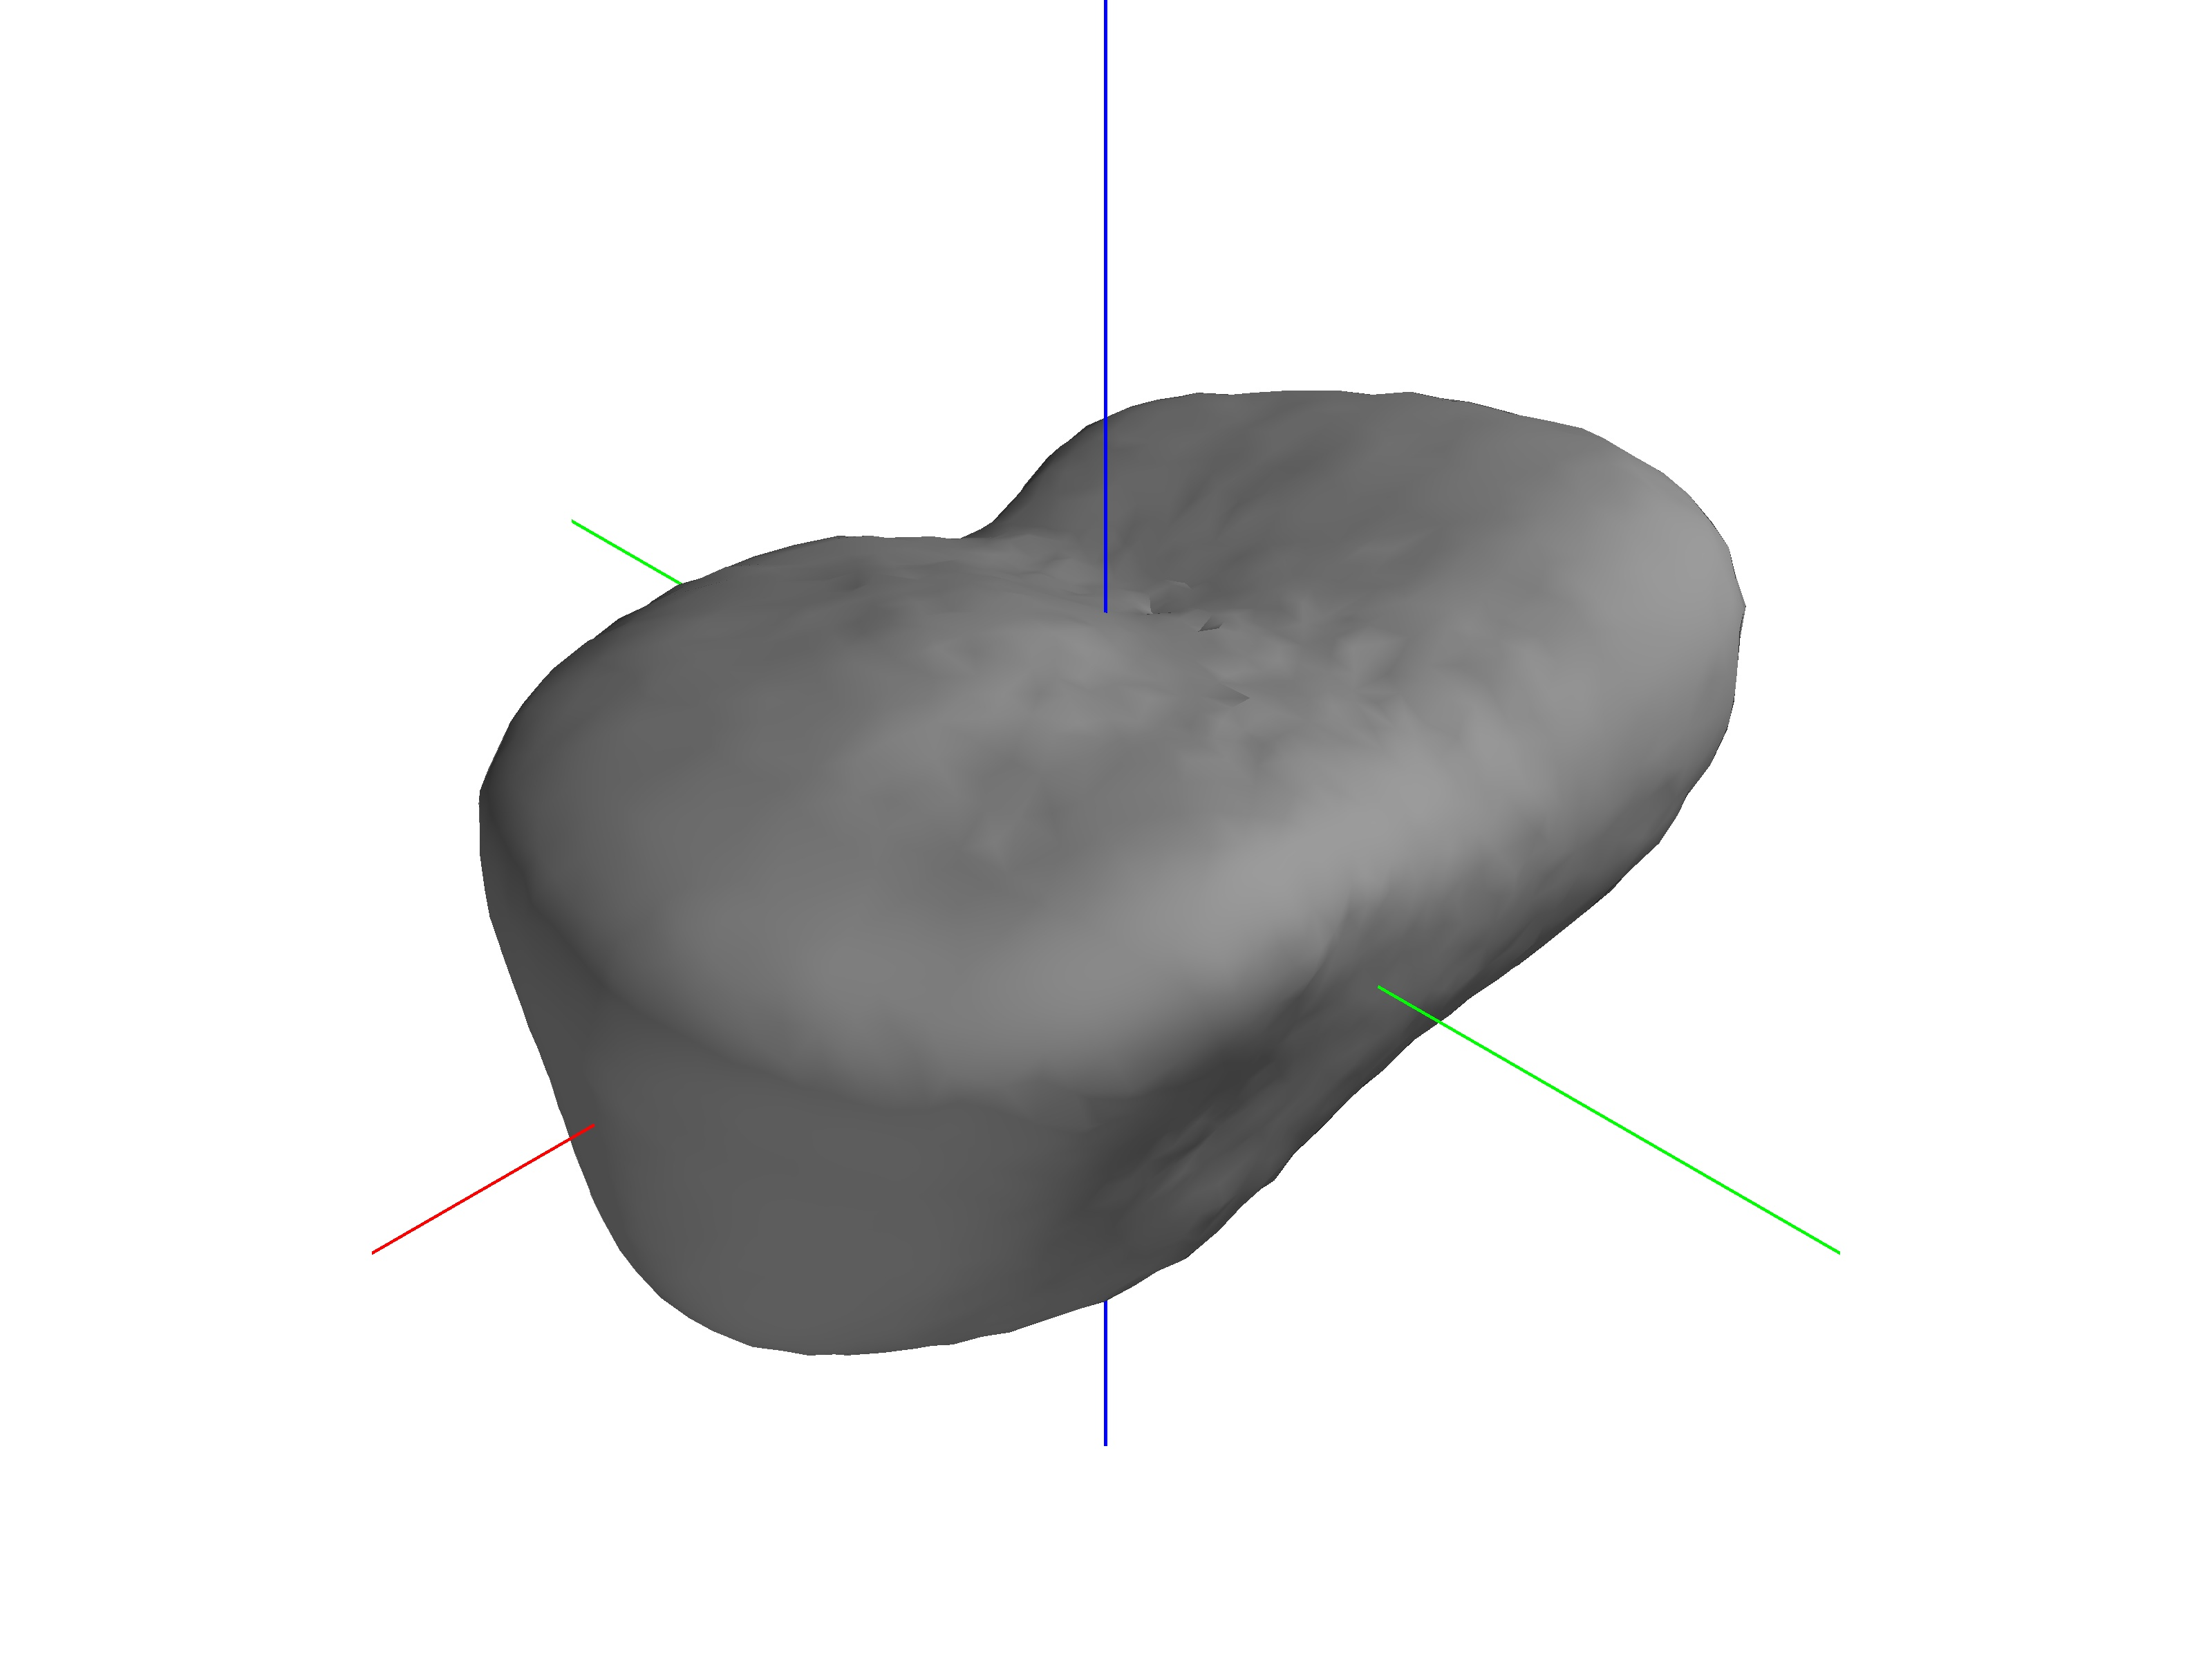
\includegraphics[width=0.5\textwidth]{figures/2018_SSPI/partial_2047.jpg}}
    \caption{4769 Castalia incremental reconstruction. The initial ellipsoid is incrementally modified by radially moving each vertex to best match the measurements.~\label{fig:reconstruction}}
\end{figure}
\section{Autonomous Mapping Guidance}\label{sec:explore_asteroid}

The mesh update algorithm presented in~\cref{sec:radius_update} does not offer a method to determine which portion of the surface needs to be updated. 
In this section, we present a computationally efficient approach to surface mapping and trajectory generation.
Utilizing the nonlinear controllers developed in~\cref{sec:se3_control} allows the spacecraft to manuever to the best location that will update the shape estimate.
Utilizing this approach enables autonomous operations at the asteroid. 

The ideal guidance approach involves solving a global optimal control problem which satisfies the system dynamics from~\cref{sec:dumbbell_model} while minimizing the shape uncertainty.
There are a wide variety of optimal control techniques which may be utilized to solve the problem, such as indirect methods~\cite{kirk2012,bryson1975}.
However, regardless of the method an optimal control formulation will result in a more computationally demanding algorithm.
Since the \gls{lidar} will be operating at upwards of \SI{1}{\hertz} efficient processing of the measurement and computation of the guidance commands is critical.

We define a cost associated with each vertex \( \vc{v}_i \) of the shape estimateas
\begin{align}\label{eq:explore_cost}
    J_i (\ipos) = \alpha_w J_{w_i} + \alpha_d J_{d_i}(\ipos) + \alpha_c J_{c_i}(\ipos)
\end{align}
where the weighting factors \( \alpha_w, \alpha_d, \alpha_c \in \R^1 \) are chosen such that \( \alpha_w + \alpha_d + \alpha_c = 1 \).
The term \( J_{w_i} \in \R^1 \) represents the cost associated with the uncertainty of vertex \( i \) as
\begin{align}\label{eq:weight_cost}
    J_{w_i} &= - \frac{w_i}{w_m}
\end{align}
where \( w_i \) is the uncertainty of vertex \( i \) and \( w_m \) is a maximum uncertainty used to scale the values.
The term \( J_{d_i} \) represents the scaled geodesic distance between the current state of the spacecraft and vertex \( i \),
\begin{align}\label{eq:distance_cost}
    J_{d_i}(\ipos) &= \frac{1}{\pi} \arctan \parenth{ \frac{\norm{\ipos \times \vc{v}_i}}{\ipos \cdot \vc{v}_i}}.
\end{align}

Finally, a control component is included in the cost function which penalizes vertices that are difficult to reach.
Consider, the current position of the spacecraft in the asteroid fixed frame as \( \rpos\) and a desired vertex \( \vc{v}_i \) of the shape estimate.
We can define a normal vector to the plane spanned by \( \rpos, \vc{v}_i \) as
\begin{align}\label{eq:normal_to_plane}
    \vc{n}_i = \frac{\rpos \times \vc{v}_i}{\norm{\rpos} \norm{\vc{v}_i}}.
\end{align}
Then a trajectory \( x_d(\theta) \) as
\begin{align}\label{eq:spherical_waypoint}
    x_d(\theta) = r_d \exp{\parenth{\theta \hat{\vc{n}_i}} } \frac{\rpos}{\norm{\rpos}},
\end{align}
where \( \theta : \bracket{0, \frac{\rpos \cdot \vc{v}_i}{\norm{\rpos}\norm{\vc{v}_i}}} \to \R^1\) parameterizes the desired trajectory.
\Cref{eq:spherical_waypoint} simply describes a portion of a great circle trajectory between the current state, \( \rpos \), and the desired vertex \( \vc{v}_i \)~\cite{chen2016}.
The altitude of the spacecraft, \( r_d \in \R \), can be chosen based on sensor characterisitics of safety concerns.
For example, \( r_d \) can be chosen as the distance of the Biroullin sphere with an additional safety margin to mitigate any surface collision.
The translational controller presented in~\cref{eq:translational_control} is used to determine the magnitude of the control to follow \( x_d\).
We assume that the tracking errors are small, such that \( e_x, e_v \) are negligible, therefore the control becomes
\begin{align}\label{eq:tracking_control_cost}
    u_f(\theta) = -F_{ext}(x_d(\theta)), 
\end{align}
where the external force is defined by the polyhedron potential model given in~\cref{eq:inertial_velocity_dynamics}.
The control cost is then defined as the integral over the desired trajectory~\cref{eq:spherical_waypoint} between the current state and the desired vertex as
\begin{align}\label{eq:control_cost}
    J_{c_i}(\rpos) = \frac{1}{u_m} \int_{\theta_0}^{\theta_f} u_f(\theta)^T R u_f(\theta) d\theta,
\end{align}
where \( u_m \) is used to normalize and scale \( J_{c_i} \).
\Cref{eq:control_cost} is numerically integrated over the trajectory \( x_d(t) \) and used to penalize vertices which have a larger cost.

The vertex which minimizes~\cref{eq:explore_cost} 
\begin{align*}
    \vc{v}_{min} = \min_{\vc{v}_i} J,
\end{align*}
is determined and used to determine the desired position of the spacecraft in the asteroid fixed frame.
The terminal state is transformed into the inertial frame and chosen as a point above \( \vc{v}_{min} \) as
\begin{align}
    \rpos = r_d \aatt \vc{v}_{min}, 
\end{align}
where \( r_d \) is again chosen to ensure a safety margin above the surface.
The desired attitude command, \( R_d\), is chosen such that the spacecraft camera axis, \( \vc{b}_1 \), is directed along the nadir towards the asteroid.
It is sufficient to define two orthogonal vectors to uniquely determine the attitude of the spacecraft.
The \( \vc{b}_{3d} \) vector is chosen to lie in the plane spanned by \(\vc{b}_{1d} \) and \( \vc{e}_3 = \vc{f}_3 \).
The desired attitude command is defined as
\begin{align}
    \vb{b}_{1d} &= - \frac{\vb{x}}{\norm{\vb{x}}} , \\
    \vb{b}_{3d} &= \frac{\vb{f}_3 - \parenth{\vb{f}_3 \cdot \vb{b}_{1d}} \vb{b}_{1d}}{\norm{\vb{f}_3 - \parenth{\vb{f}_3 \cdot \vb{b}_{1d}} \vb{b}_{1d}}}, \\
    \vb{b}_{2d} &= \vb{b}_{3d} \times \vb{b}_{1d} , \\
R_d &= \begin{bmatrix} \vb{b}_{1d} & \vb{b}_{2d} & \vb{b}_{3d} \end{bmatrix} .
\end{align}
The camera axis is aligned with the spacecraft \( \vb{b}_ 1 \) axis, which is direted towards the asteroid, throughout the trajectory.

\subsection{Landing Area Refinement}\label{sec:landing_refinement}
The shape update approach presented in~\cref{sec:radius_update} is designed with autonomous operations in mind. 
It is based on an initial coarse shape estimate that is iteratively updated with range measurements of the surface.
Furthermore, the original mesh is uniformly distributed and as a result many small topological features such as rocks or small craters are not be captured by the shape model. 
However, these small features are critical for surface operations and safe landings.
In addition, it would be computationaly prohibitive to have a uniformly high resolution mesh.
In this section, we extend the previous shape update approach to enable a much higher fidelity in a specific location.

Mixed resolution surface meshes are routinely used in finite element and geometric modeling applications~\cite{botsch2010}.
As shown in~\cite{mcmahon2017}, utilizing mixed resolution shape models for asteroid missions offers the potential of reduced computational demands.
The computational cost of the polyhedron potential model given by~\cref{eq:potential} is roughly proporitional to the number of faces in the shape model.
As a result, a uniformly high resolution shape would quickly become intractable for realtime operations.
However, utilizing a mixed resolution approach allows for a high fidelity in a smaller mission critical area, such as a landing site, with a limited impact on the computational cost.

The selection of a landing site will typically require a vast quantity of data and weigh a multitude of possible metrics, such as scientific value, hardware constraints, timing and communication limits, or safety considerations. 
In our analysis we consider the surface slope, the distance to the surface, and a fictitious science metric in order to determine the best landing site based on the complete shape estimate.
This approach allows for a spacecraft to autonomously select and land on an asteroid.

The surface slope is computed according to the method developed in~\cite{scheeres1996}.
Due to the small size, and therefore low gravitational attraction, the force at each point on the surface is a combination of the gravitational attraction and the centripital acceleration.
At the center of each face, \( f_i = \begin{bmatrix} f_x & f_y & f_z \end{bmatrix} \), we compute a modified surface acceleration as
\begin{align}\label{eq:surface_force}
    U_m = \omega^2 \begin{bmatrix} f_x \\ f_y \\ 0 \end{bmatrix} + \begin{bmatrix} U_x \\ U_y \\ U_z \end{bmatrix},
\end{align}
where \( \omega \in \R^1 \) is the angular velocity of the asteroid and \( U_i \) is computed from~\cref{eq:attraction}.
Then the surface slope can be computed from
\begin{align}\label{eq:surface_slope}
    \cos \parenth{ \pi - \phi } = \frac{\vc{n}_f \cdot U_m}{\norm{U_m}},
\end{align}
where \( \phi \in \R^1 \) is the surface slope defines the angle between the surface normal \( \vc{n}_f \in \R^3 \) and the force vector at the surface.
If \( \phi = \SI{0}{\degree} \) then the force vector and the surface normal are anti-parallel, while \( \phi > \SI{90}{\degree} \) means that a particle on the surface would be thrown off the body as the centripetal force is larger than the gravitational attraction.
\begin{figure}[htbp]
    \centering
    \includegraphics[width=\textwidth]{example-image-golden}
    \caption[Estimate Surface slope of 4769 Castalia]{Estimated surface slope of asteroid 4769 Castalia~\label{fig:surface_slope_castalia}}
\end{figure}
Additionally, we compute the distance, using~\cref{eq:geodesic_distance}, between the spacecraft state and each face of the asteroid. 
Finally, we also assign a random science value to the surface in the form of two dimensional Gaussian.
Utilizing these metric, a landing site is chosen to minimize the surface cost given as
\begin{align}\label{eq:surface_cost}
    J_l =  J_{\text{distance}} - J_{\text{science}},
\end{align}
where the surface slope is considered a hard constraint such that any candidate landing site must satisify \( \phi \leq \phi_m \).
Graphically, we can combine~\cref{fig:surface_slope_castalia,fig:surface_distance_castalia,fig:surface_science_castalia} to generate a single graphical representation fo of the cost function~\cref{eq:surface_cost}.

\begin{figure}[htbp]
    \centering
    \includegraphics[width=\textwidth]{example-image-golden}
    \caption[Distance to Surface]{Estimated distance to surface asteroid 4769 Castalia~\label{fig:surface_distance_castalia}}
\end{figure}

\begin{figure}[htbp]
    \centering
    \includegraphics[width=\textwidth]{example-image-golden}
    \caption[Science Value]{Science Value over the surface~\label{fig:surface_science_castalia}}
\end{figure}

\begin{figure}[htbp]
    \centering
    \includegraphics[width=\textwidth]{example-image-golden}
    \caption[Total Surface Landing Cost]{Total Landing Cost~\label{fig:surface_total_castalia}}
\end{figure}

\paragraph{Mesh Refinement}\label{sec:refinement}
Once a suitable landing site is selected the surround area is isolated and refined by adding new vertices and faces in the specified area.
The goal of refinement, or more generally remeshing, is given a mesh ( or a portion of it), compute another mesh whose elements satisfy some quality metrics while suitabably approximating the original mesh.
In this work, we utilize the isotropic remeshing algorithm implemented in \gls{cgal}.
This algorithm uses an iterative method which repeatedly splits long edges, collapses short edges, and relocates vertices until all edges are approximately the desired target edge length.
\begin{figure}[htbp]
    \centering
    \includegraphics[width=\textwidth]{example-image-golden}
    \caption[Isotropic Remeshing]{LOOK IN PMP 101 Local remeshing operations.(Image duplicated from~\cite{botsch2010})\label{fig:isotropic_remeshing}}
\end{figure}
For example,~\cref{fig:cube_remesh} shows the isotropic remeshing result for the selected faces of a cube.
Each of the new triangular faces of the mesh have approximately equal edge lengths and the surface tangent is preserved.
\begin{figure}[htbp]
    \centering
    \subcaptionbox{Original Cube\label{fig:cube_original_mesh}}{\includegraphics[width=0.5\textwidth]{example-image-golden}}~
    \subcaptionbox{Remeshed Cube\label{fig:cube_refine_mesh}}{\includegraphics[width=0.5\textwidth]{example-image-golden}}
    \caption{Example of Isotropic remeshing of a face of a cube\label{fig:cube_remesh}}
\end{figure}

The true shape model of asteroid Castalia is generated from radar imagery.
As a result, the shape model is not highly detailed as it does not contain small craters or surface features.
In order to apply the landing refinement process we agument a small portion of the mesh with some additional features and utilize the mesh update scheme in~\cref{sec:radius_update} to measure the surface.
The augmented model of Castalia is shown in~\cref{fig:bumpy_castalia}.
\begin{figure}[htbp]
    \centering
    \subcaptionbox{Original  Castalia\label{fig:orig_castalia}}{\includegraphics[width=0.5\textwidth]{example-image-golden}}~
    \subcaptionbox{Bumpy Castalia\label{fig:bump_castalia}}{\includegraphics[width=0.5\textwidth]{example-image-golden}}
    \caption{Original and Bumpy Castalia with landing features~\label{fig:bumpy_castalia}}
\end{figure}

\section{Shape Reconstruction Examples}

% TODO Metric to measure goodness of reconstruction (volume and uncertainty plots}

% TODO Show examples of shape reconstruction (Castalia, using C++ code for speed)

% TODO Show the dynamic exploration and reconstruction of Castlia and 52760

% TODO First exploration, then refinement, then landing

